\chapter{Appendix D - Machine Learning}

\section{Test Conditions and Data Summary}
\FloatBarrier

The following charts show trends in precipitation, ambient pressure, cloud cover, dew, and light level over the course of our two month MassDEP co-location test.

\begin{figure}[htb]
 	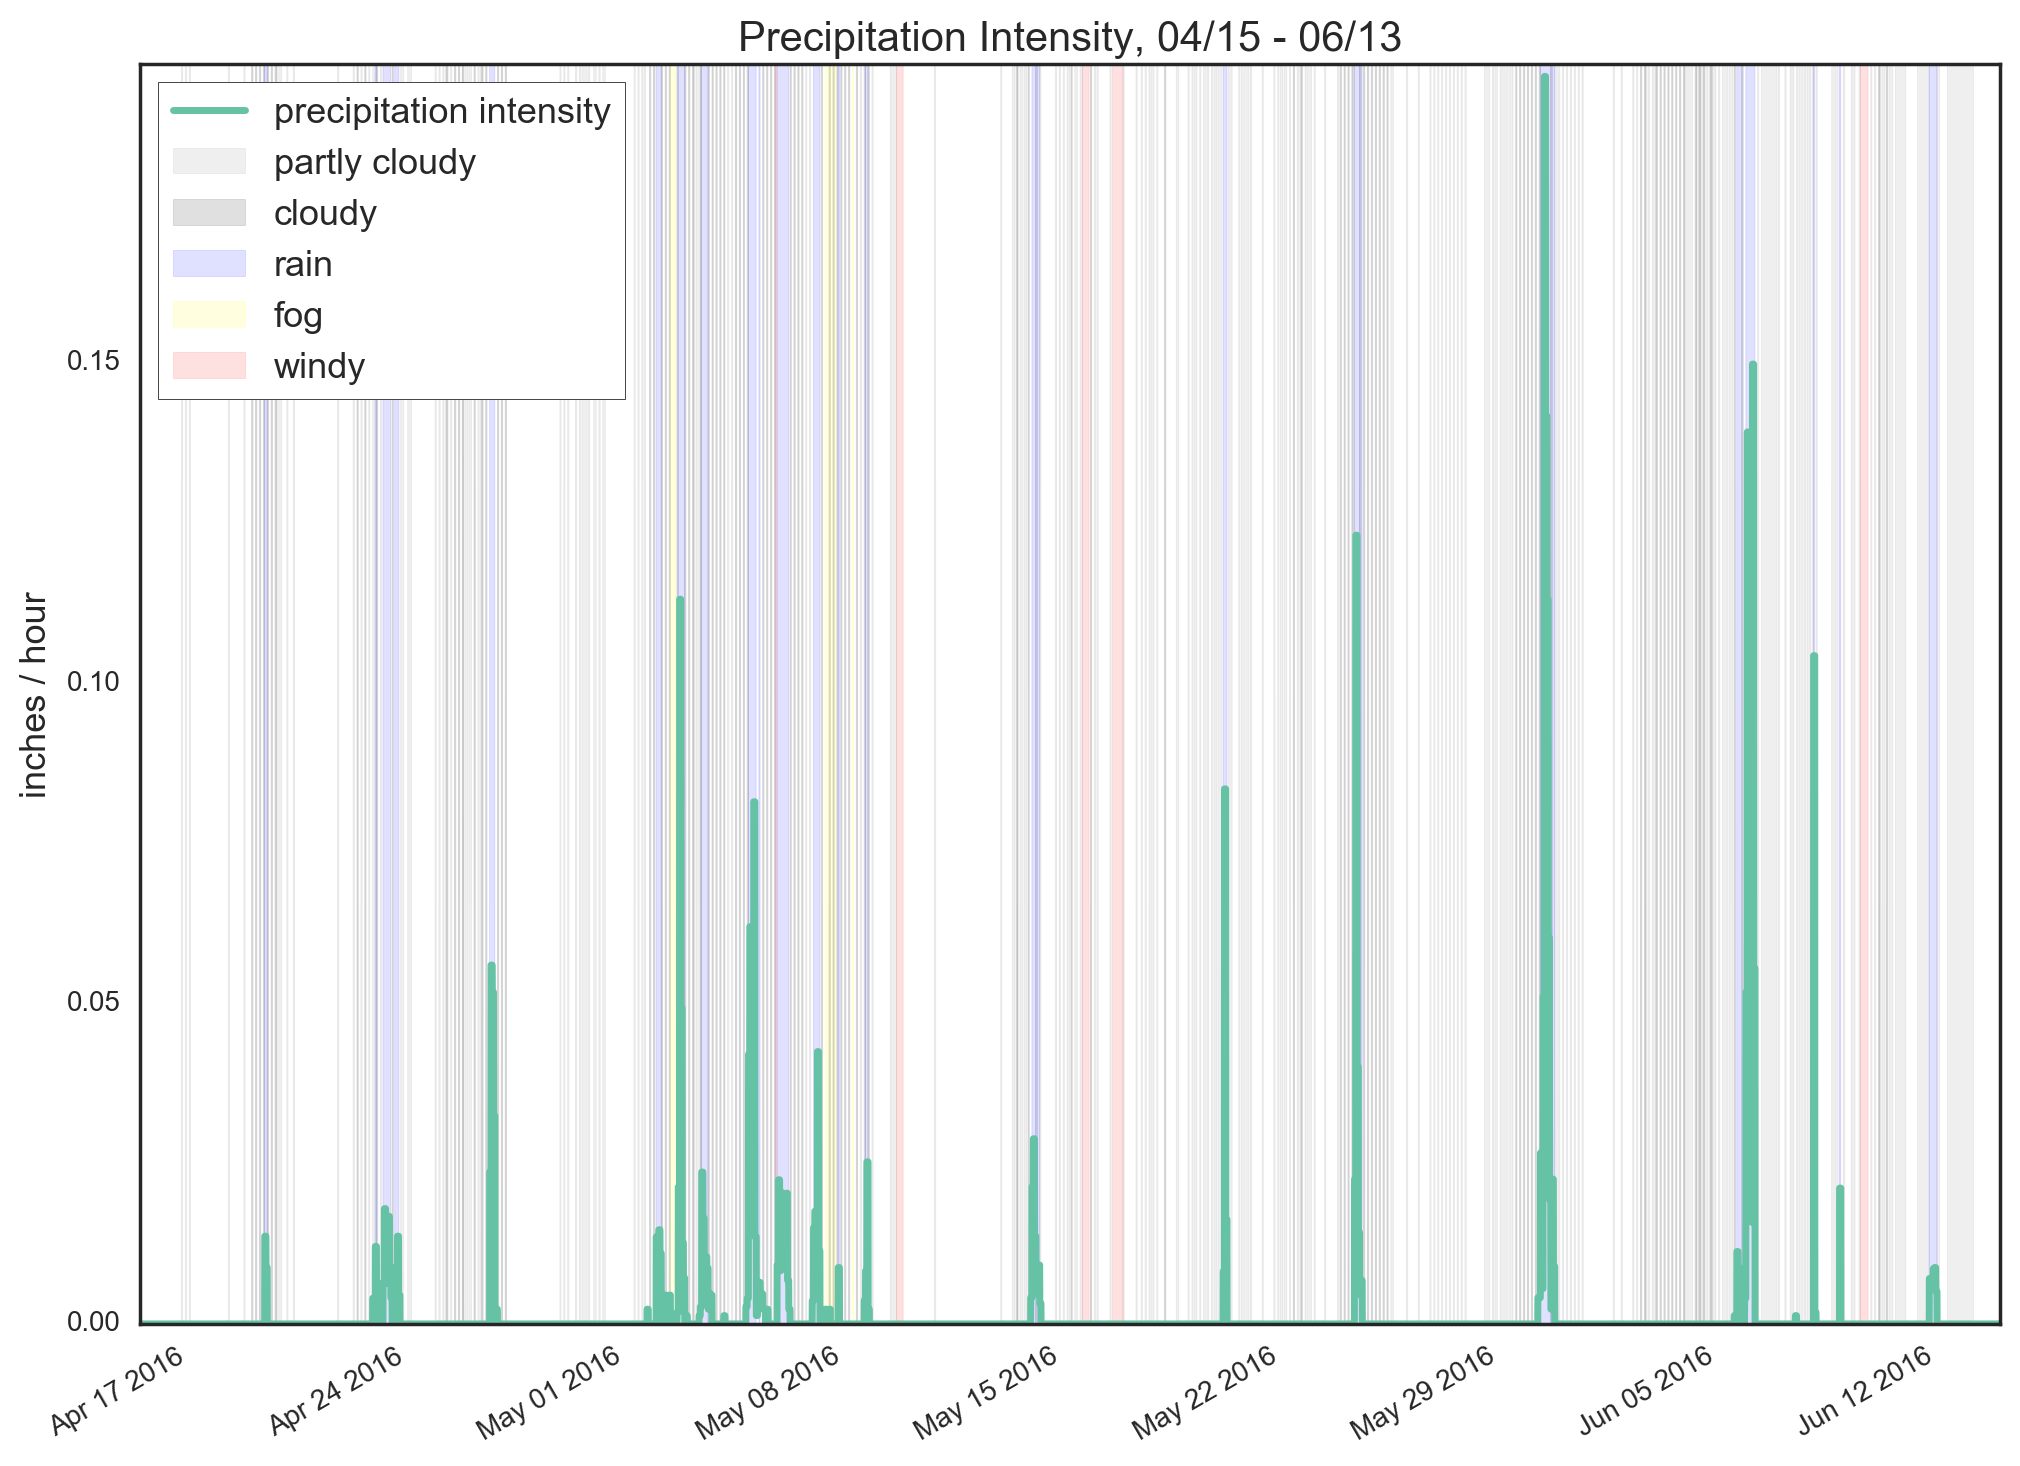
\includegraphics[width=\textwidth]{figs/precip_intensity}               
 	 \caption{Precipitation Intensity during Test Period}
  	\label{fig:precip_intensity}
\end{figure}

\begin{figure}[htb]
 	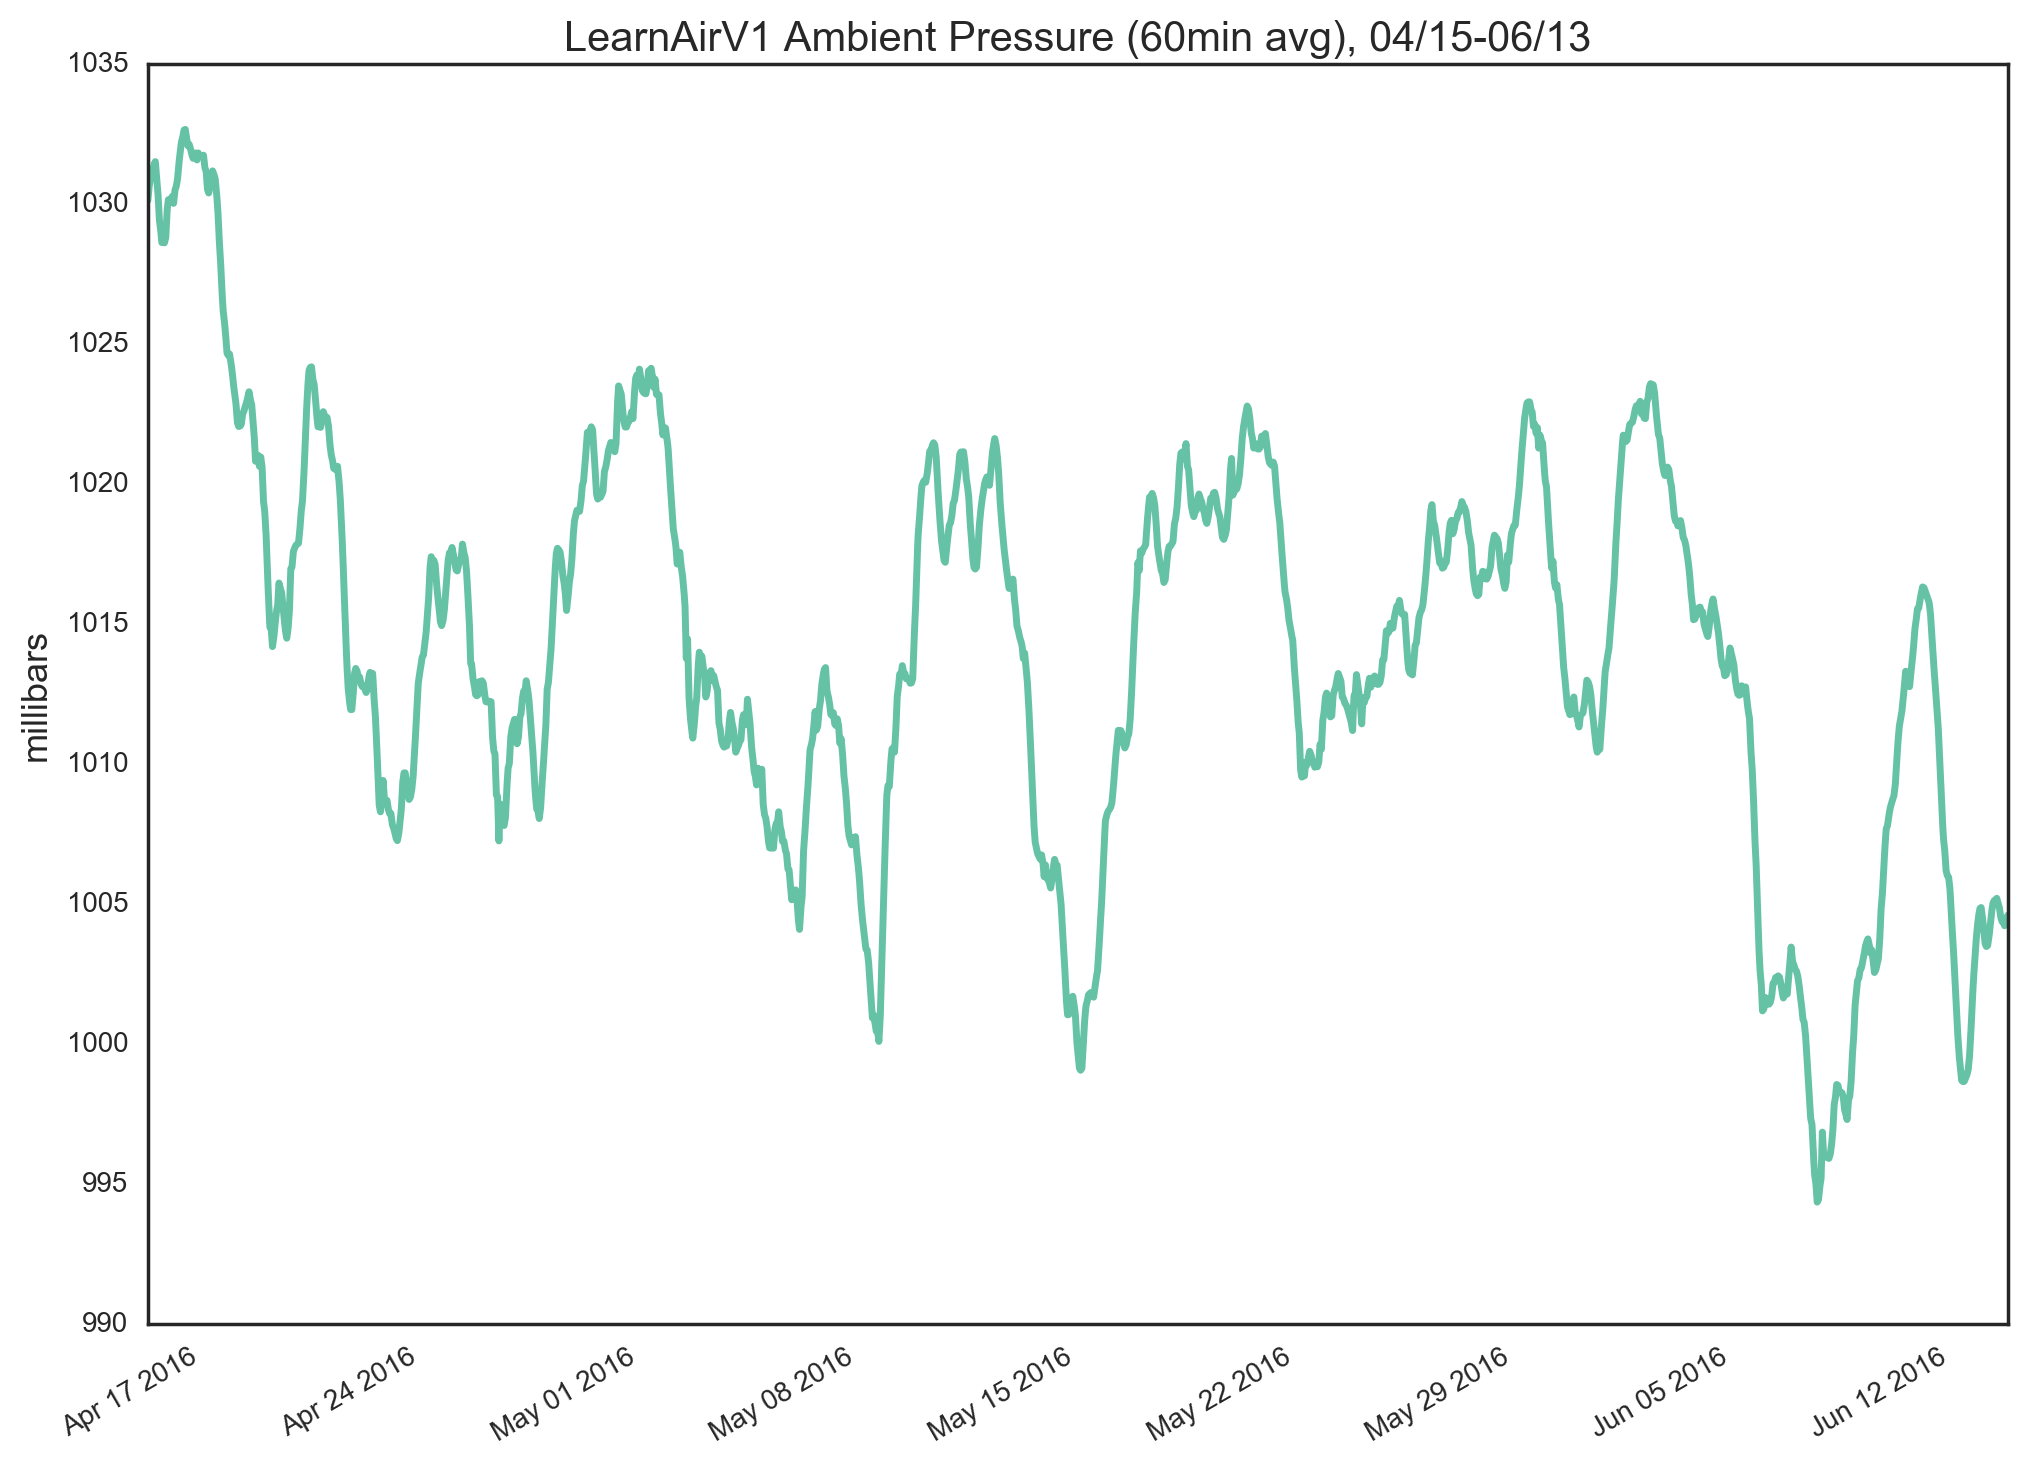
\includegraphics[width=\textwidth]{figs/ambient_pressure}               
 	 \caption{Ambient Pressure during Test Period}
  	\label{fig:ambient_pressure}
\end{figure}

\begin{figure}[htb]
 	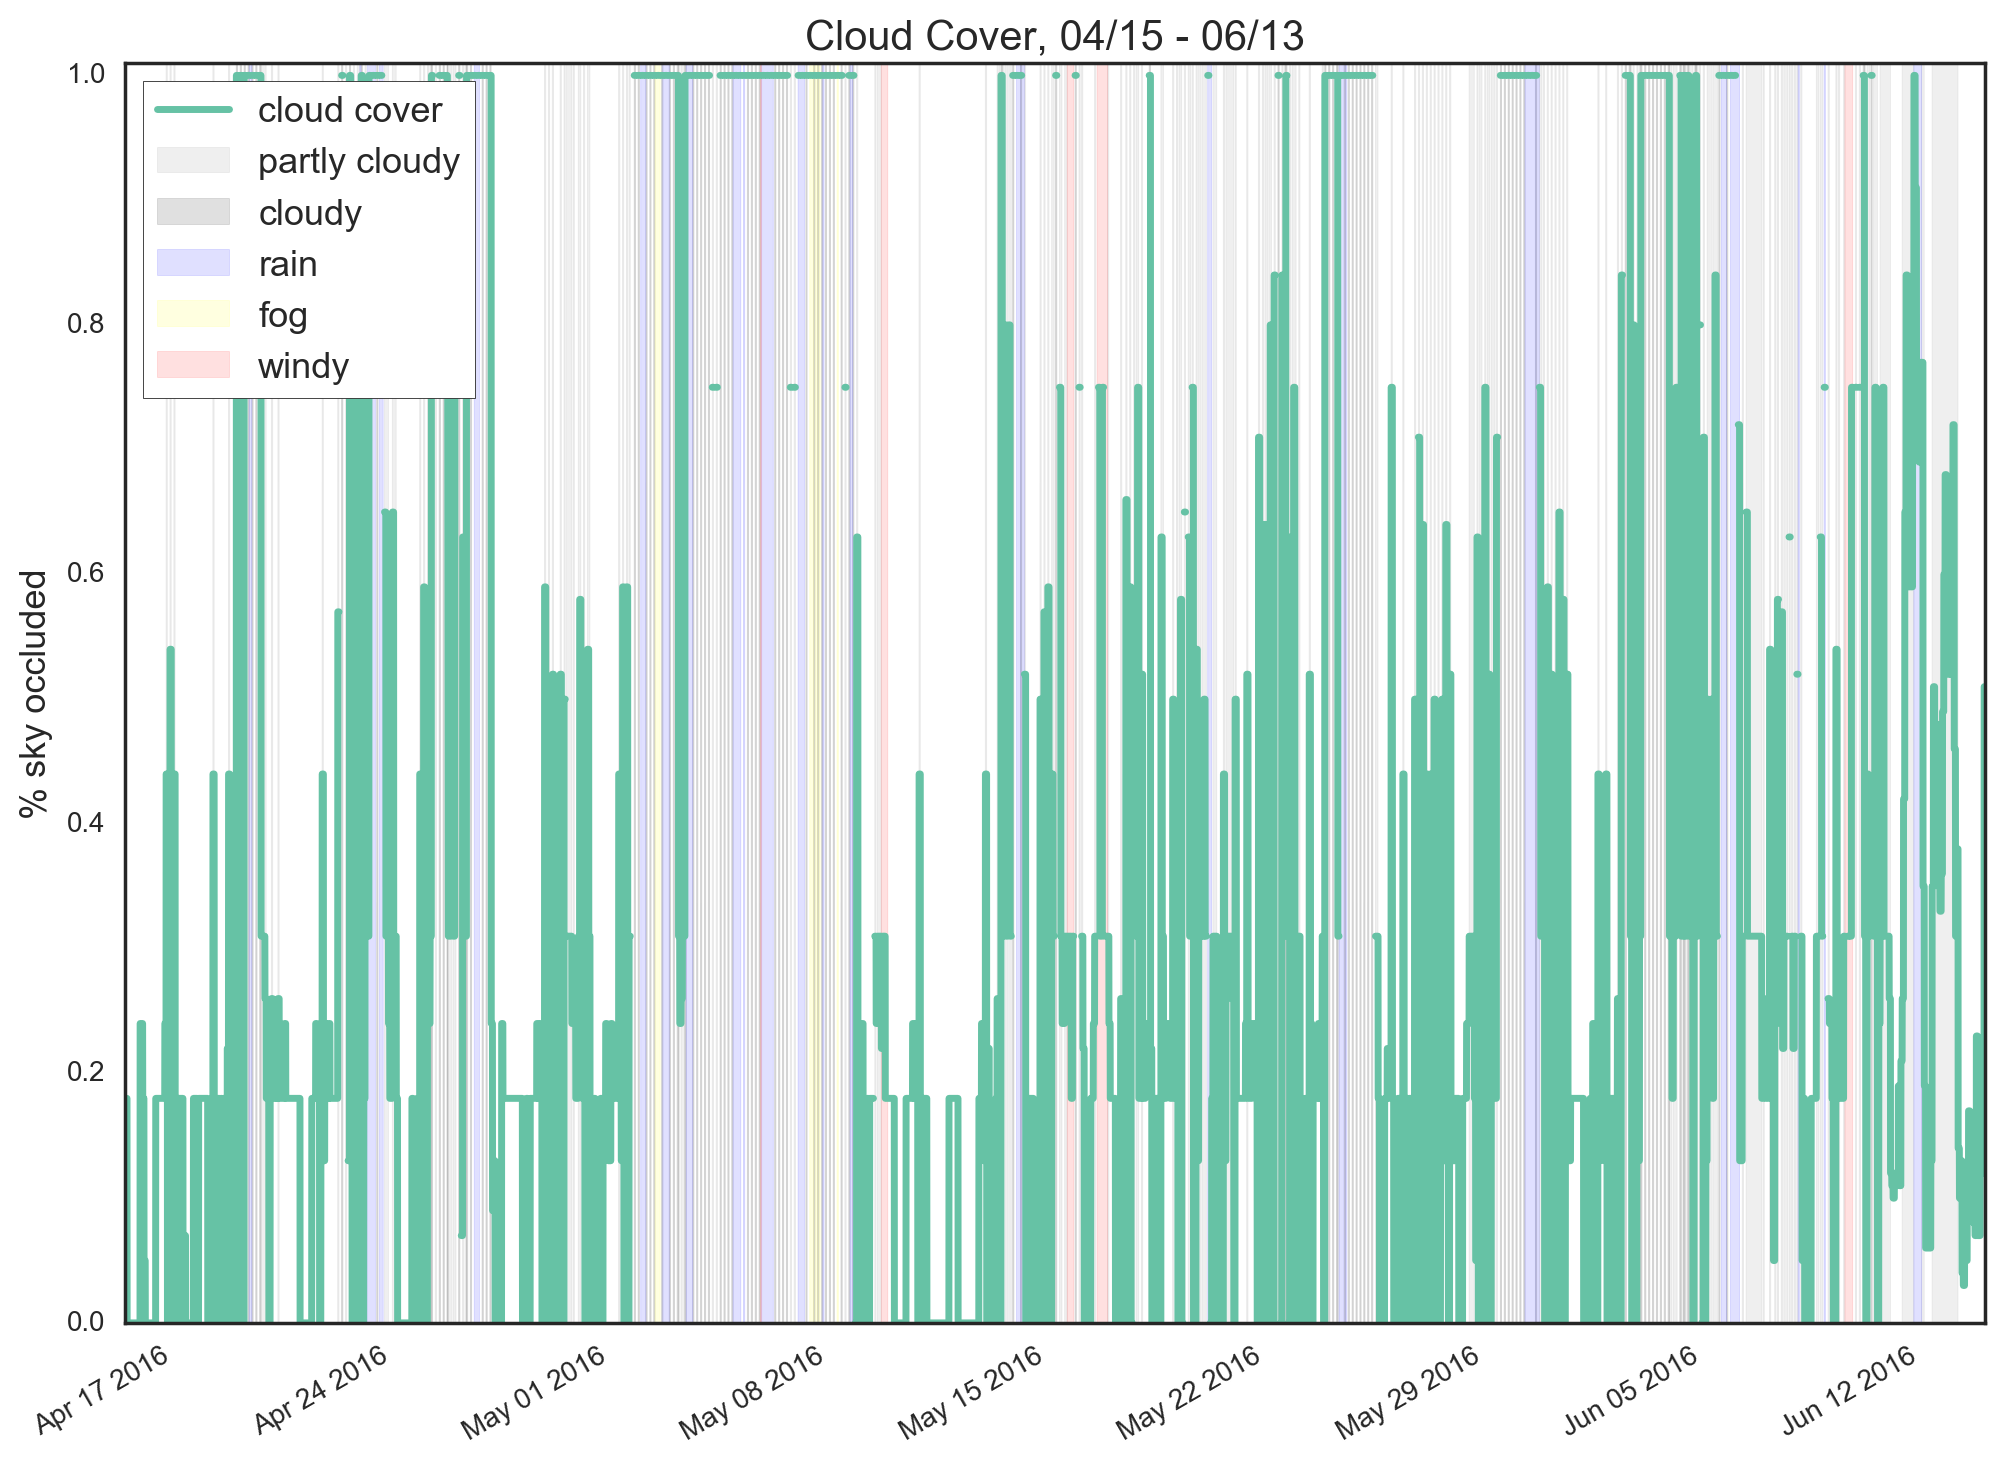
\includegraphics[width=\textwidth]{figs/cloud_cover}               
 	 \caption{Cloud Cover during Test Period}
  	\label{fig:cloud_cover}
\end{figure}

\begin{figure}[htb]
 	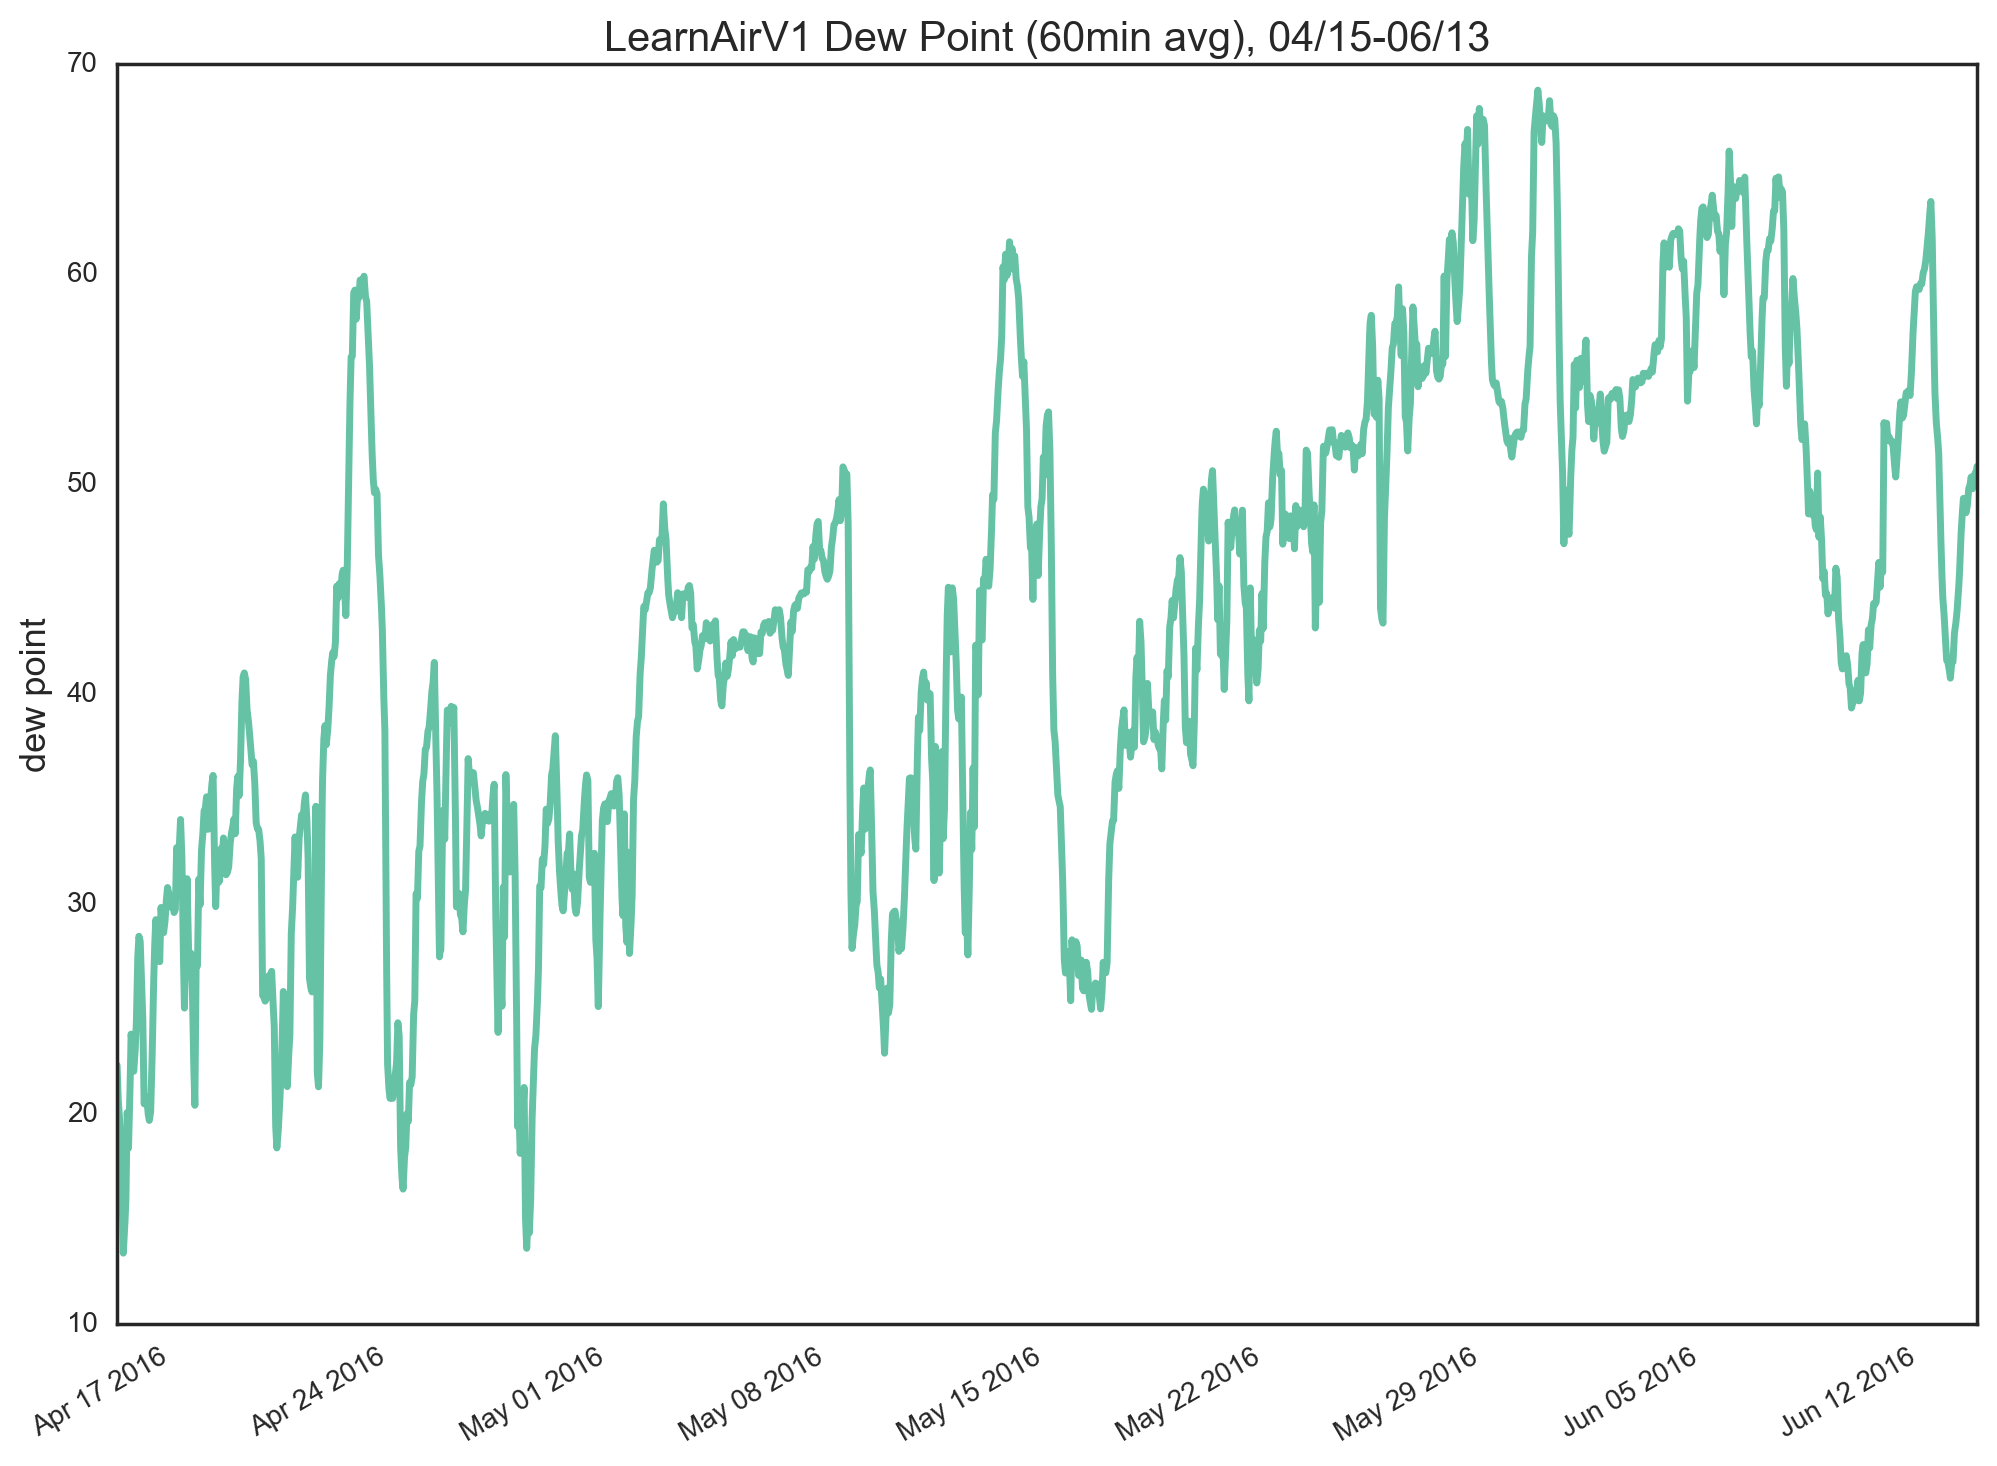
\includegraphics[width=\textwidth]{figs/dew}               
 	 \caption{Dew during Test Period}
  	\label{fig:dew}
\end{figure}

\begin{figure}[htb]
 	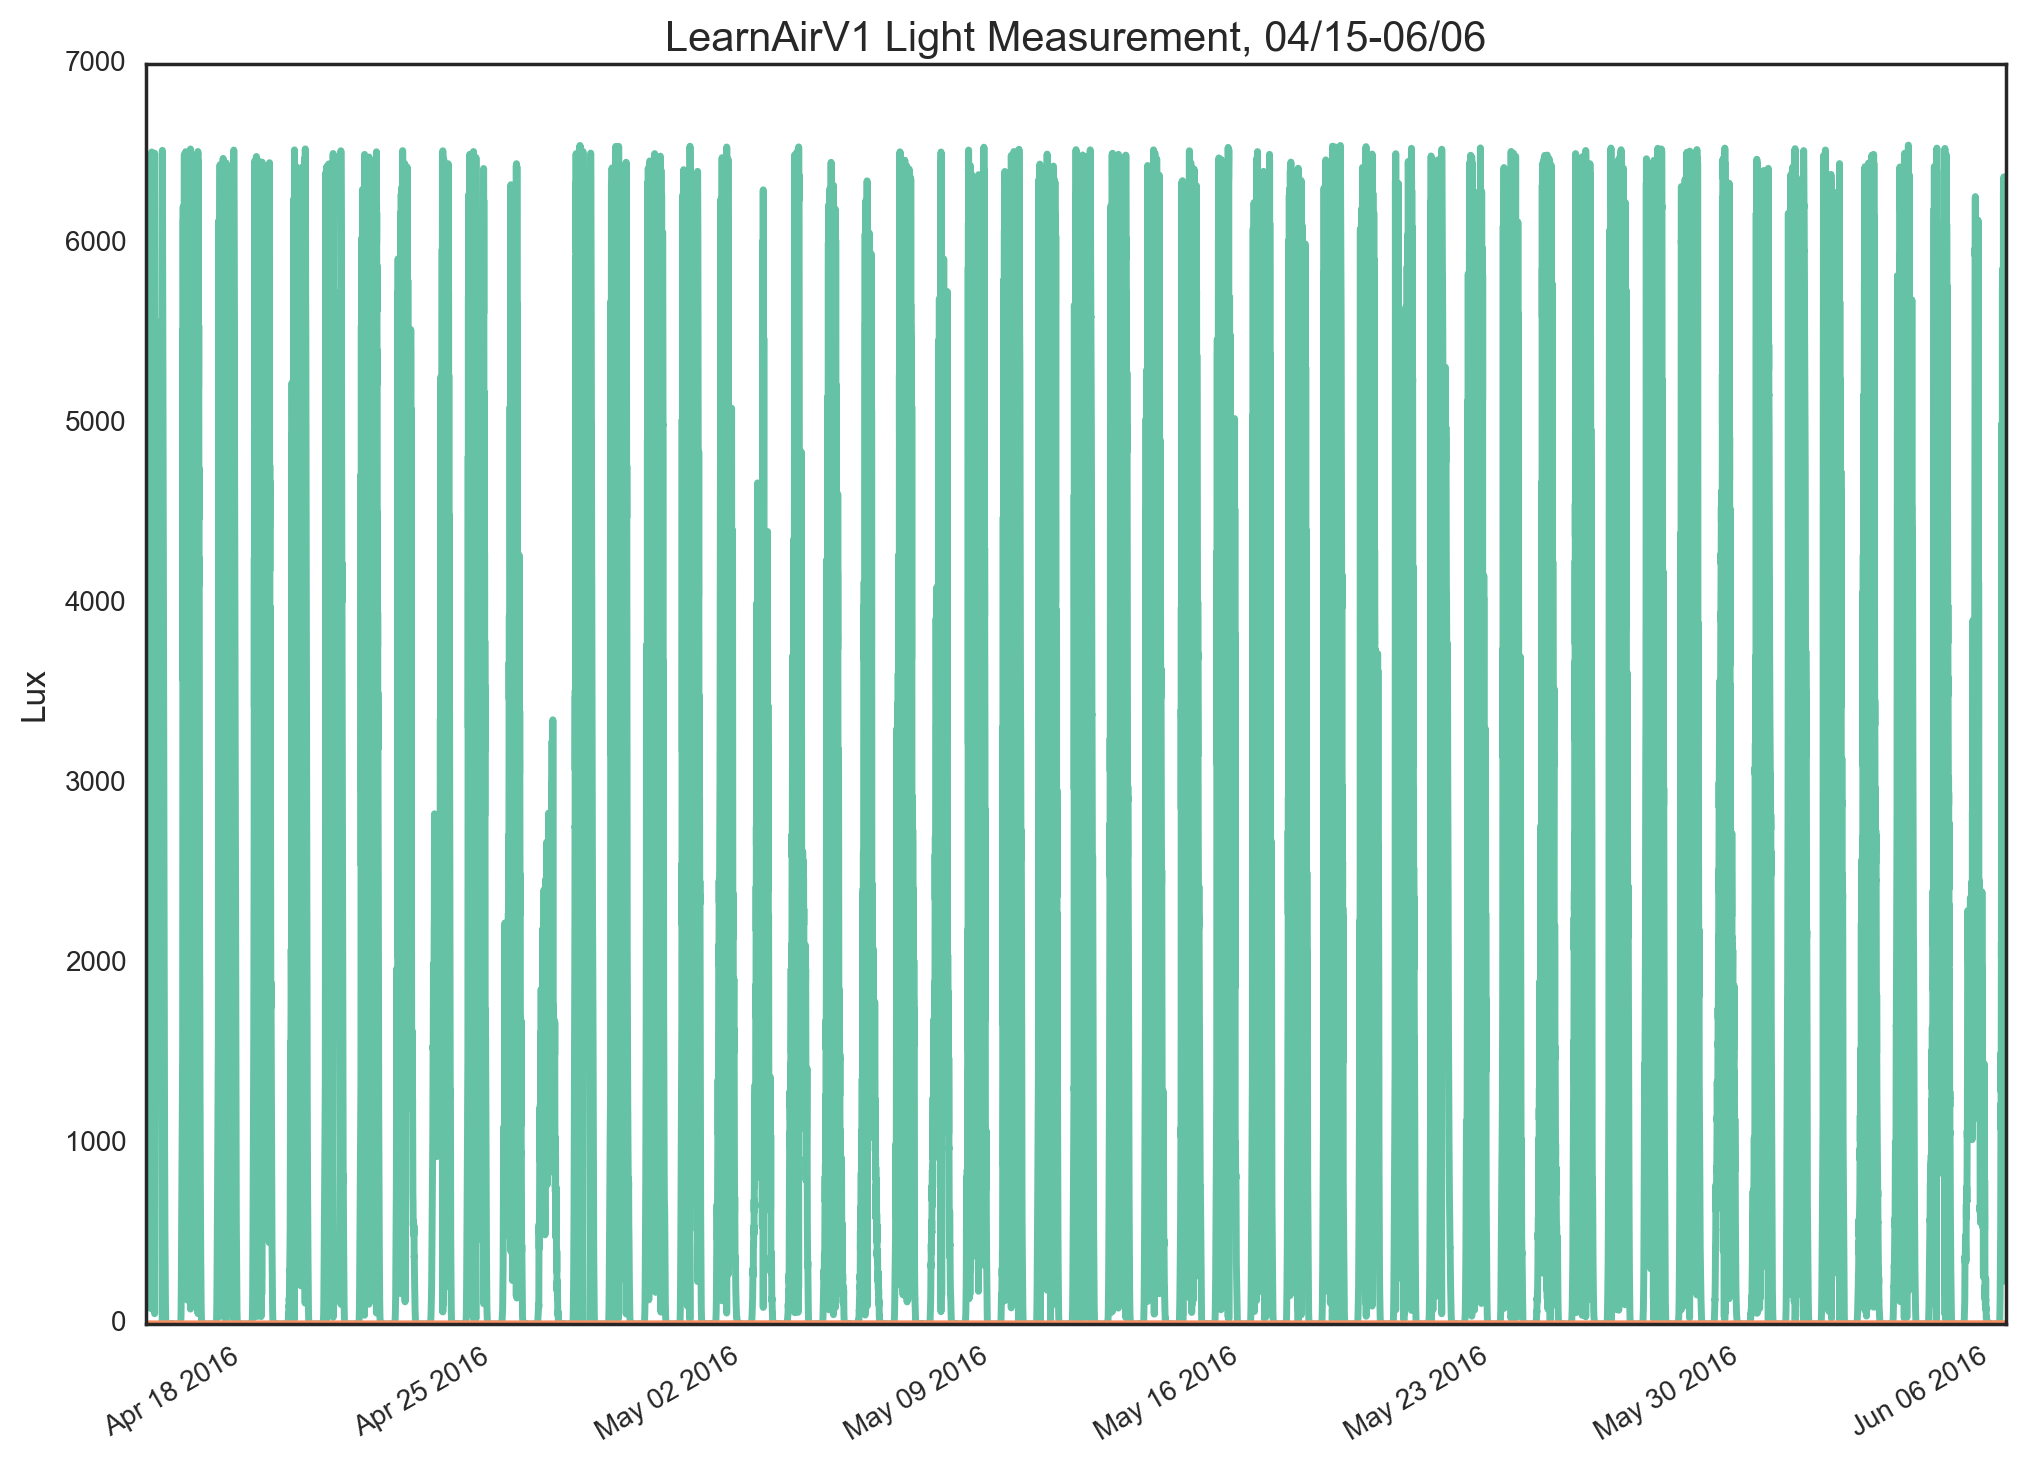
\includegraphics[width=\textwidth]{figs/lux}               
 	 \caption{Lux during Test Period}
  	\label{fig:lux}
\end{figure}

\begin{figure}[htb]
 	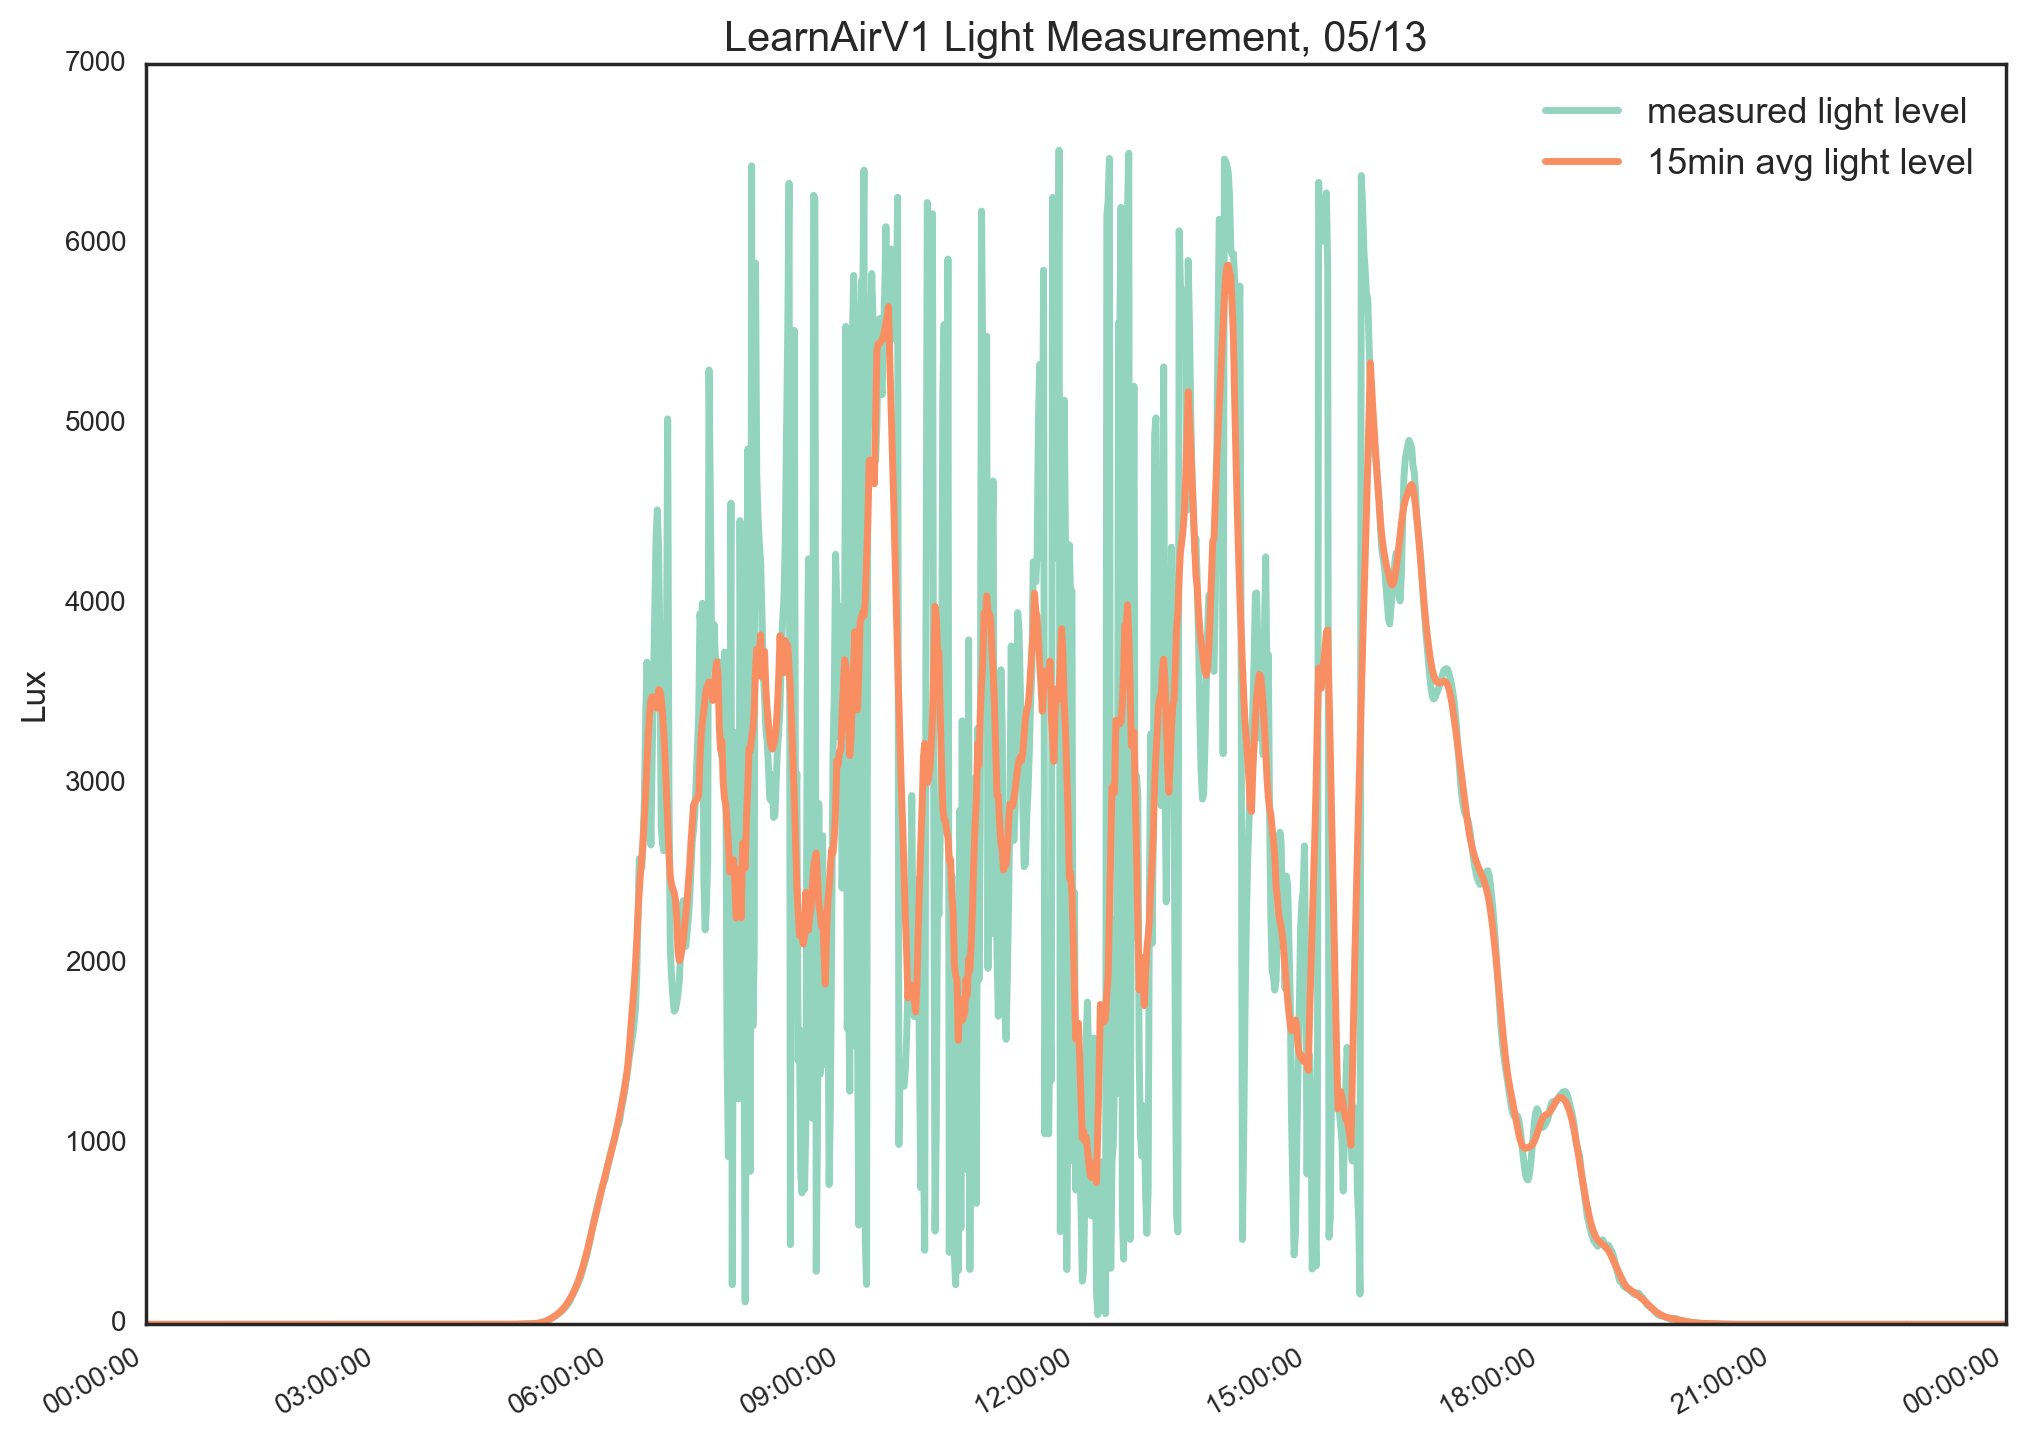
\includegraphics[width=\textwidth]{figs/lux_zoomed}               
 	 \caption{Lux during Test Period}
  	\label{fig:lux_zoomed}
\end{figure}

\FloatBarrier
\section{Data Pre-Processing}
\FloatBarrier

\FloatBarrier
\section{Features}
\FloatBarrier

Below are many of the machine learning feature distributions plotted using Weka.

\begin{figure}[htb]
 	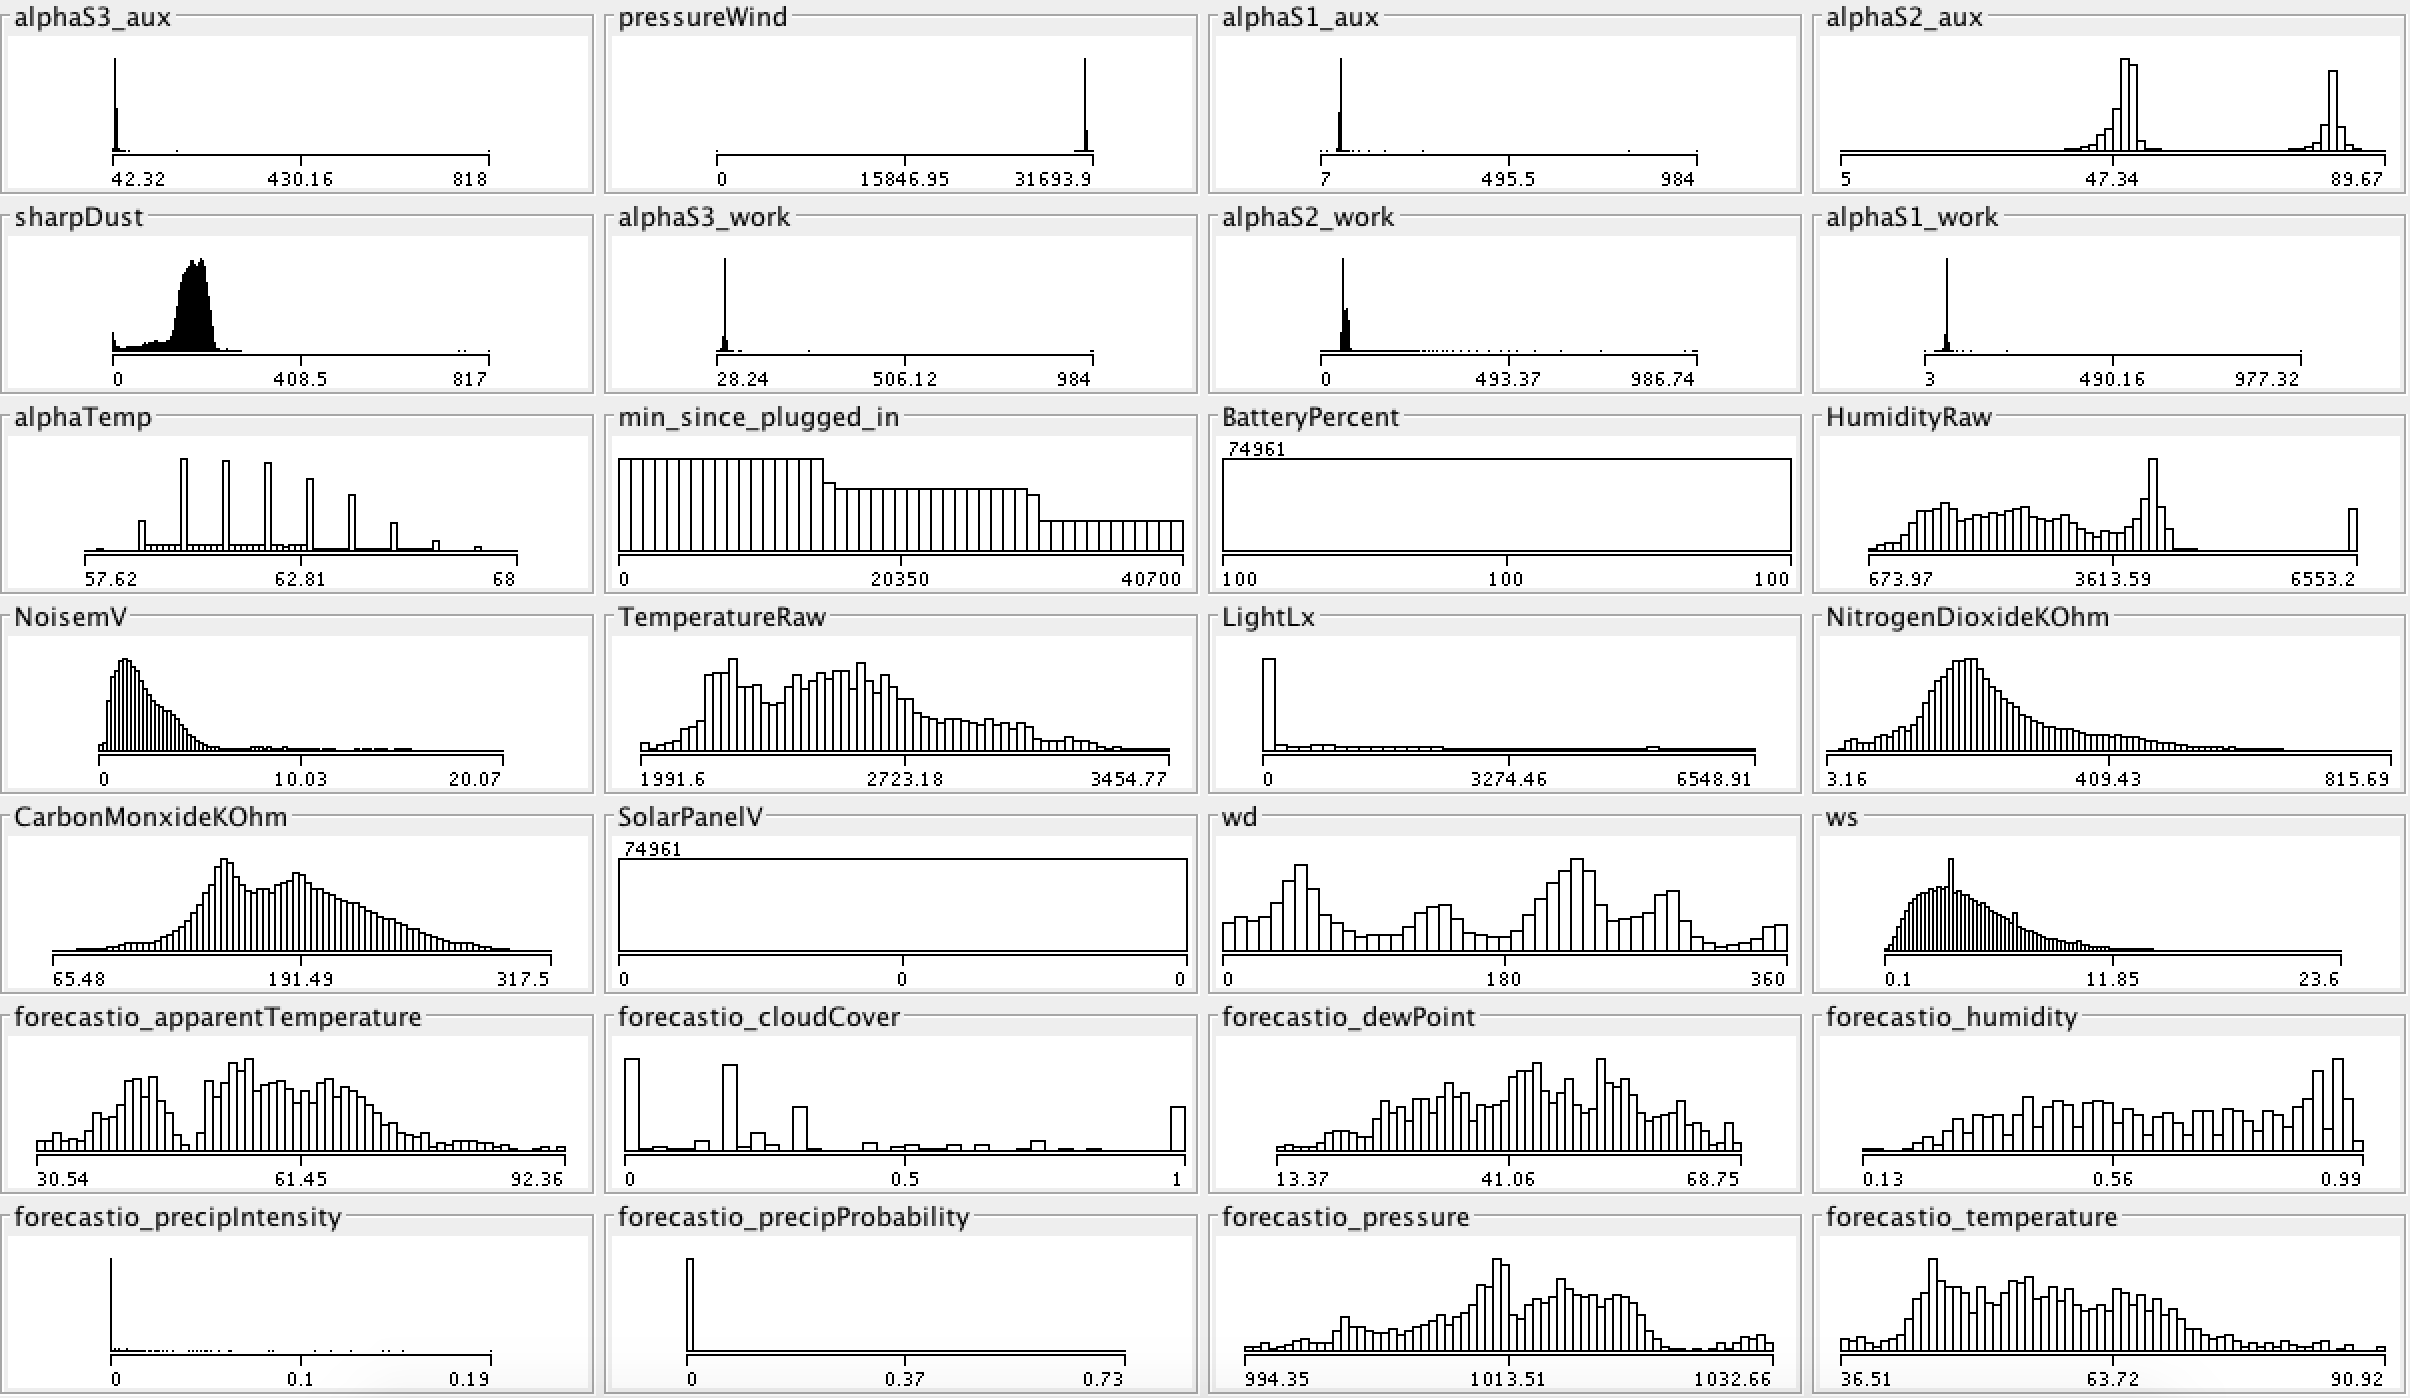
\includegraphics[width=\textwidth]{weka/features1}  
	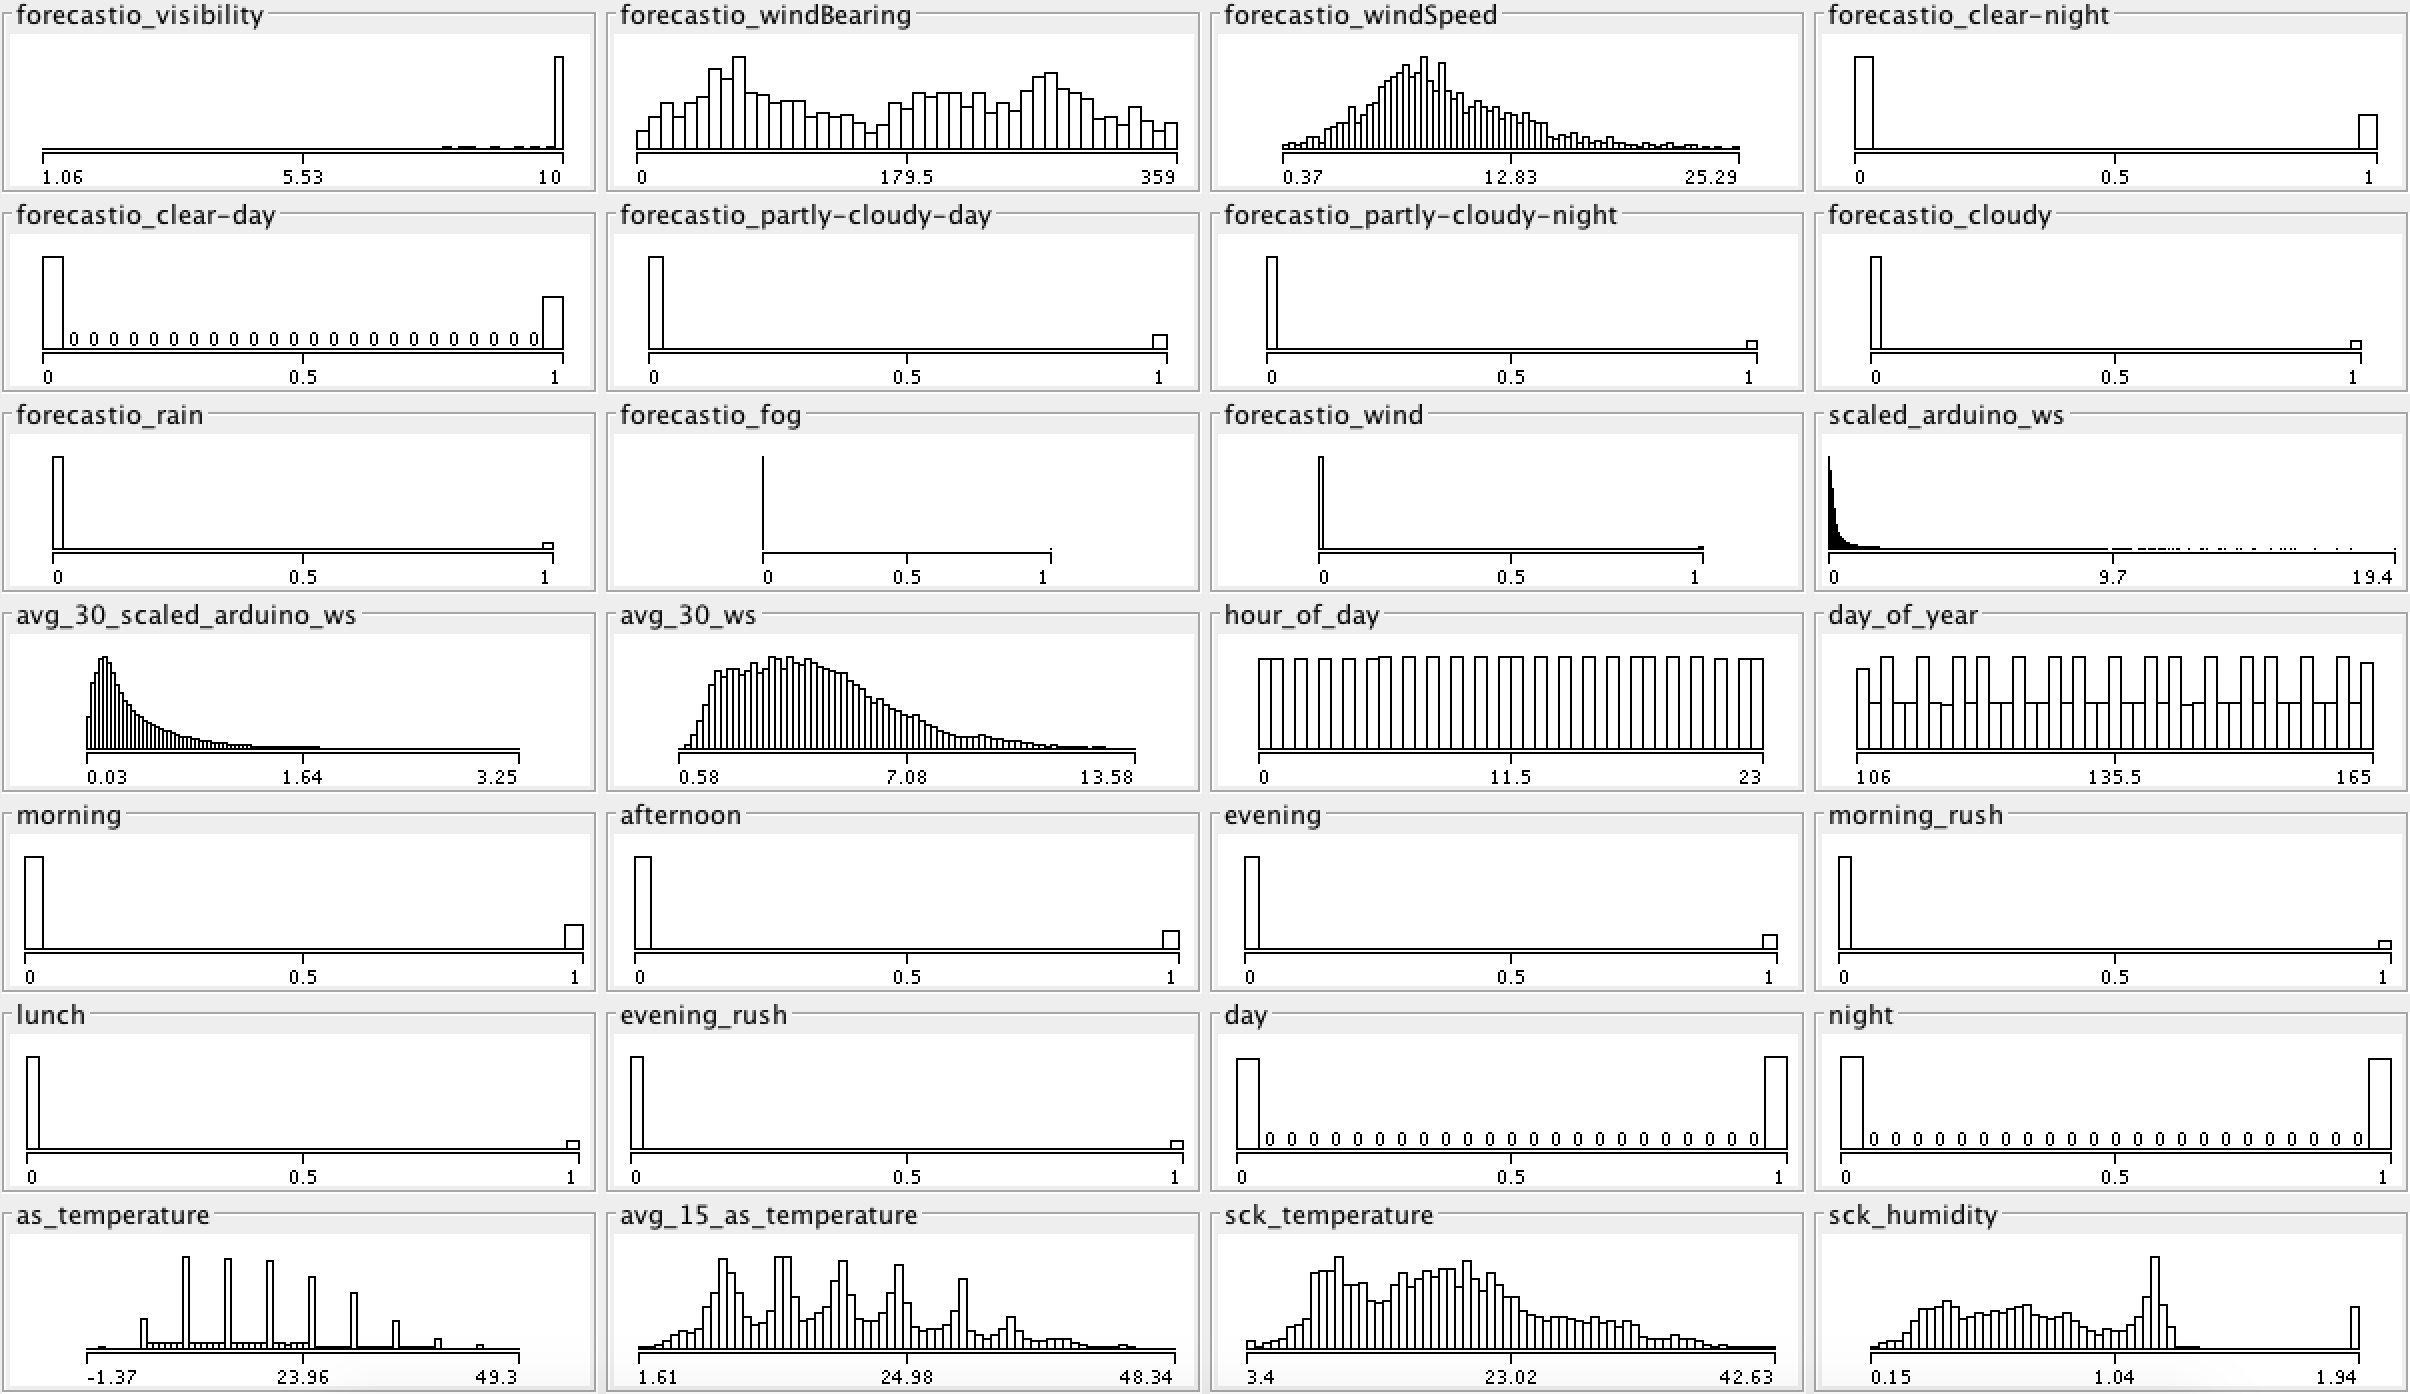
\includegraphics[width=\textwidth]{weka/features2}  
	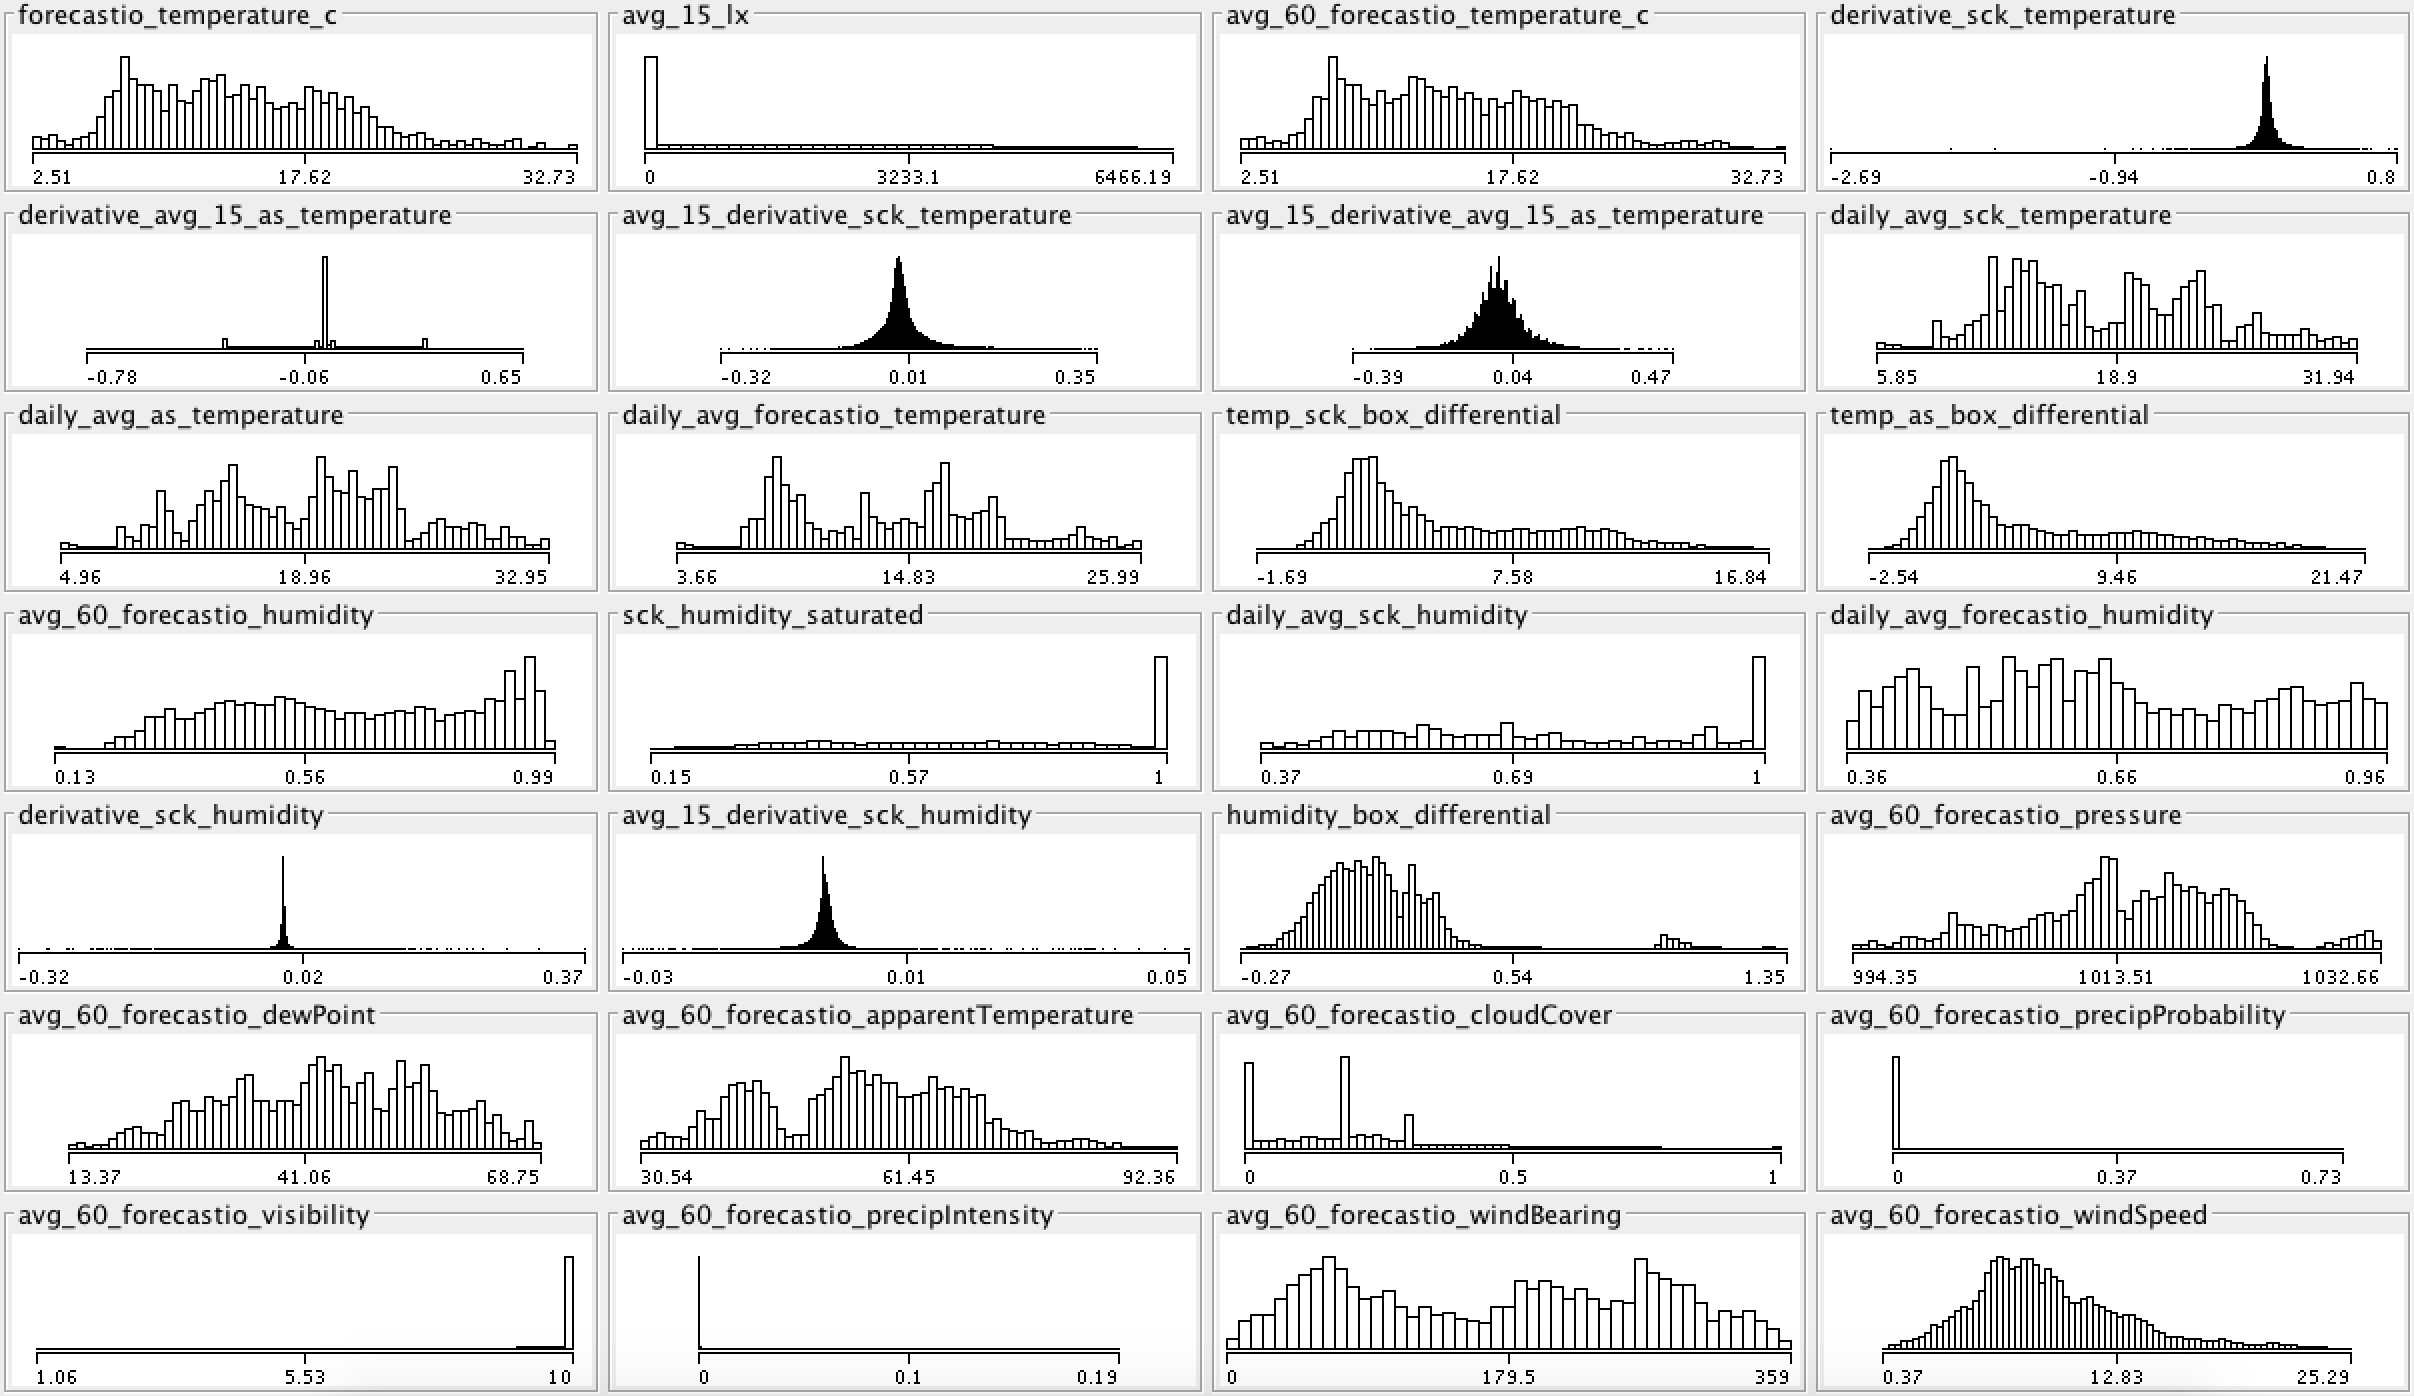
\includegraphics[width=\textwidth]{weka/features3}  
	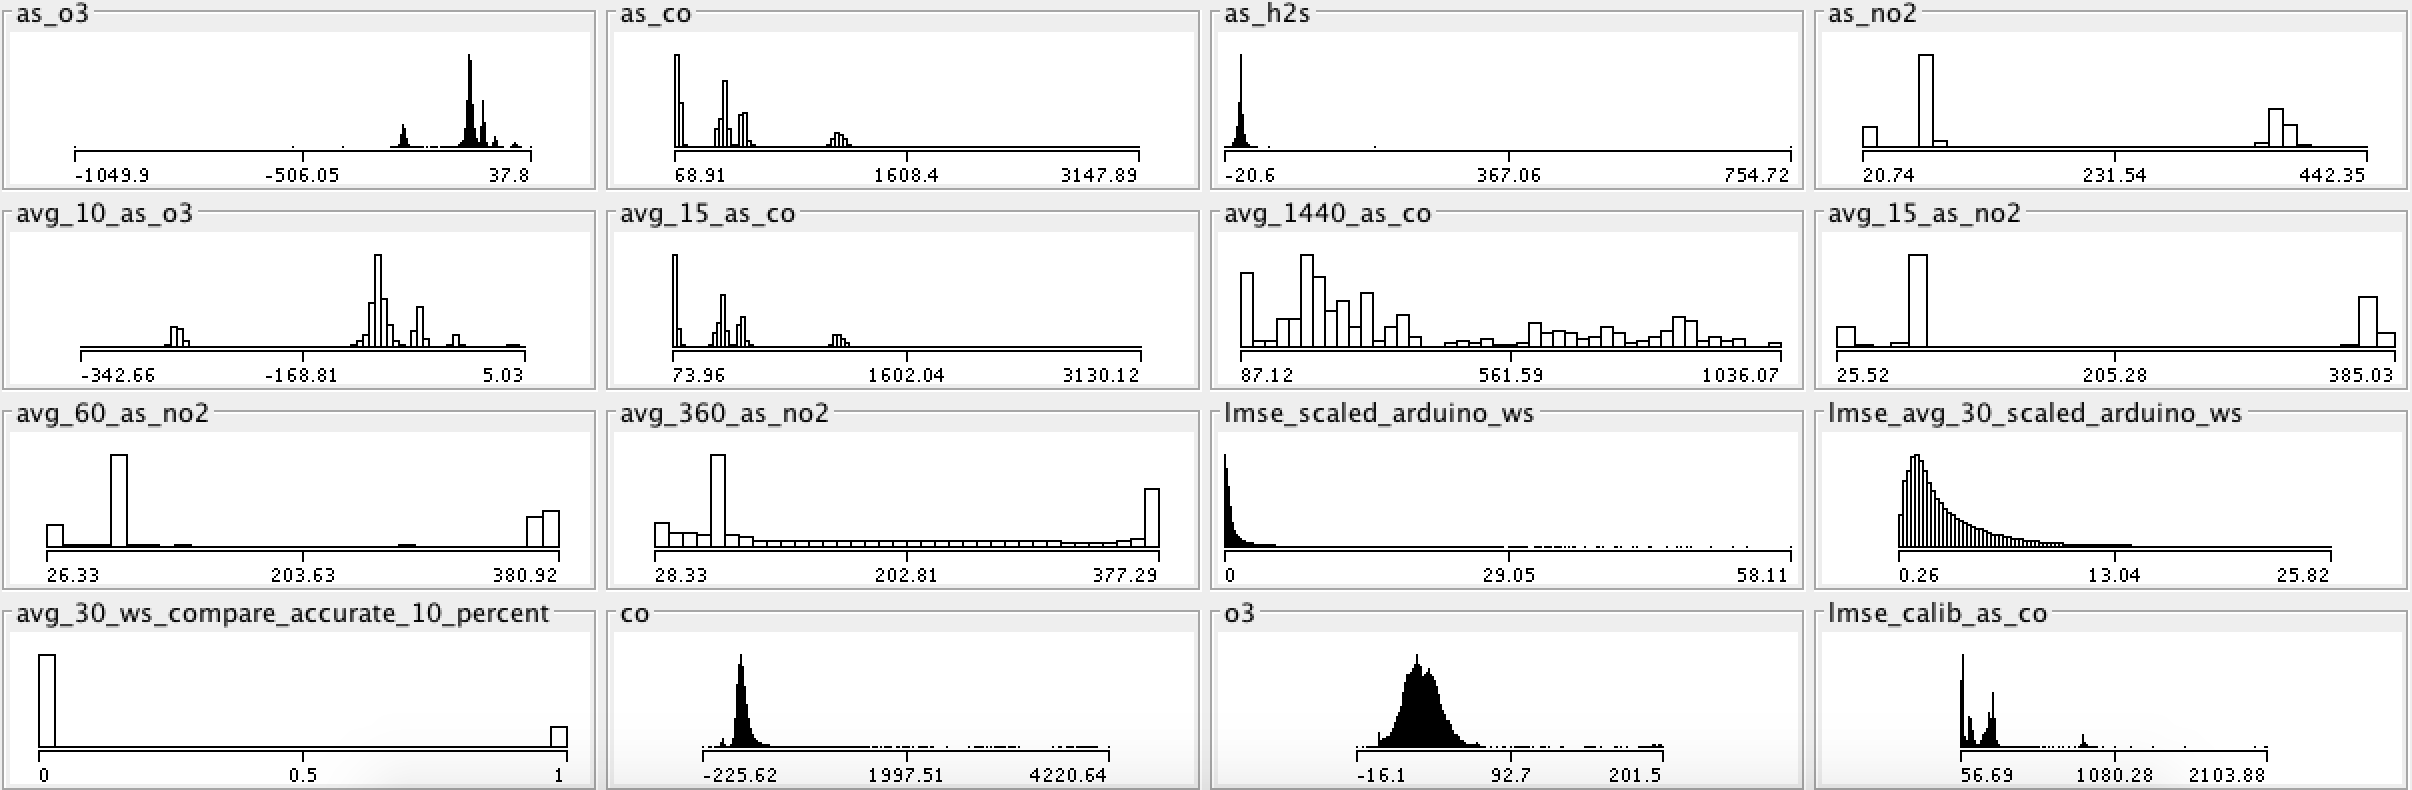
\includegraphics[width=\textwidth]{weka/features4}                 
         \caption{ML feature histograms plotted with WEKA Tool}
 	 \label{fig:weka_features}
\end{figure}

\FloatBarrier
\section{SmartCitizen CO}
\FloatBarrier

\begin{figure}[htb]
 	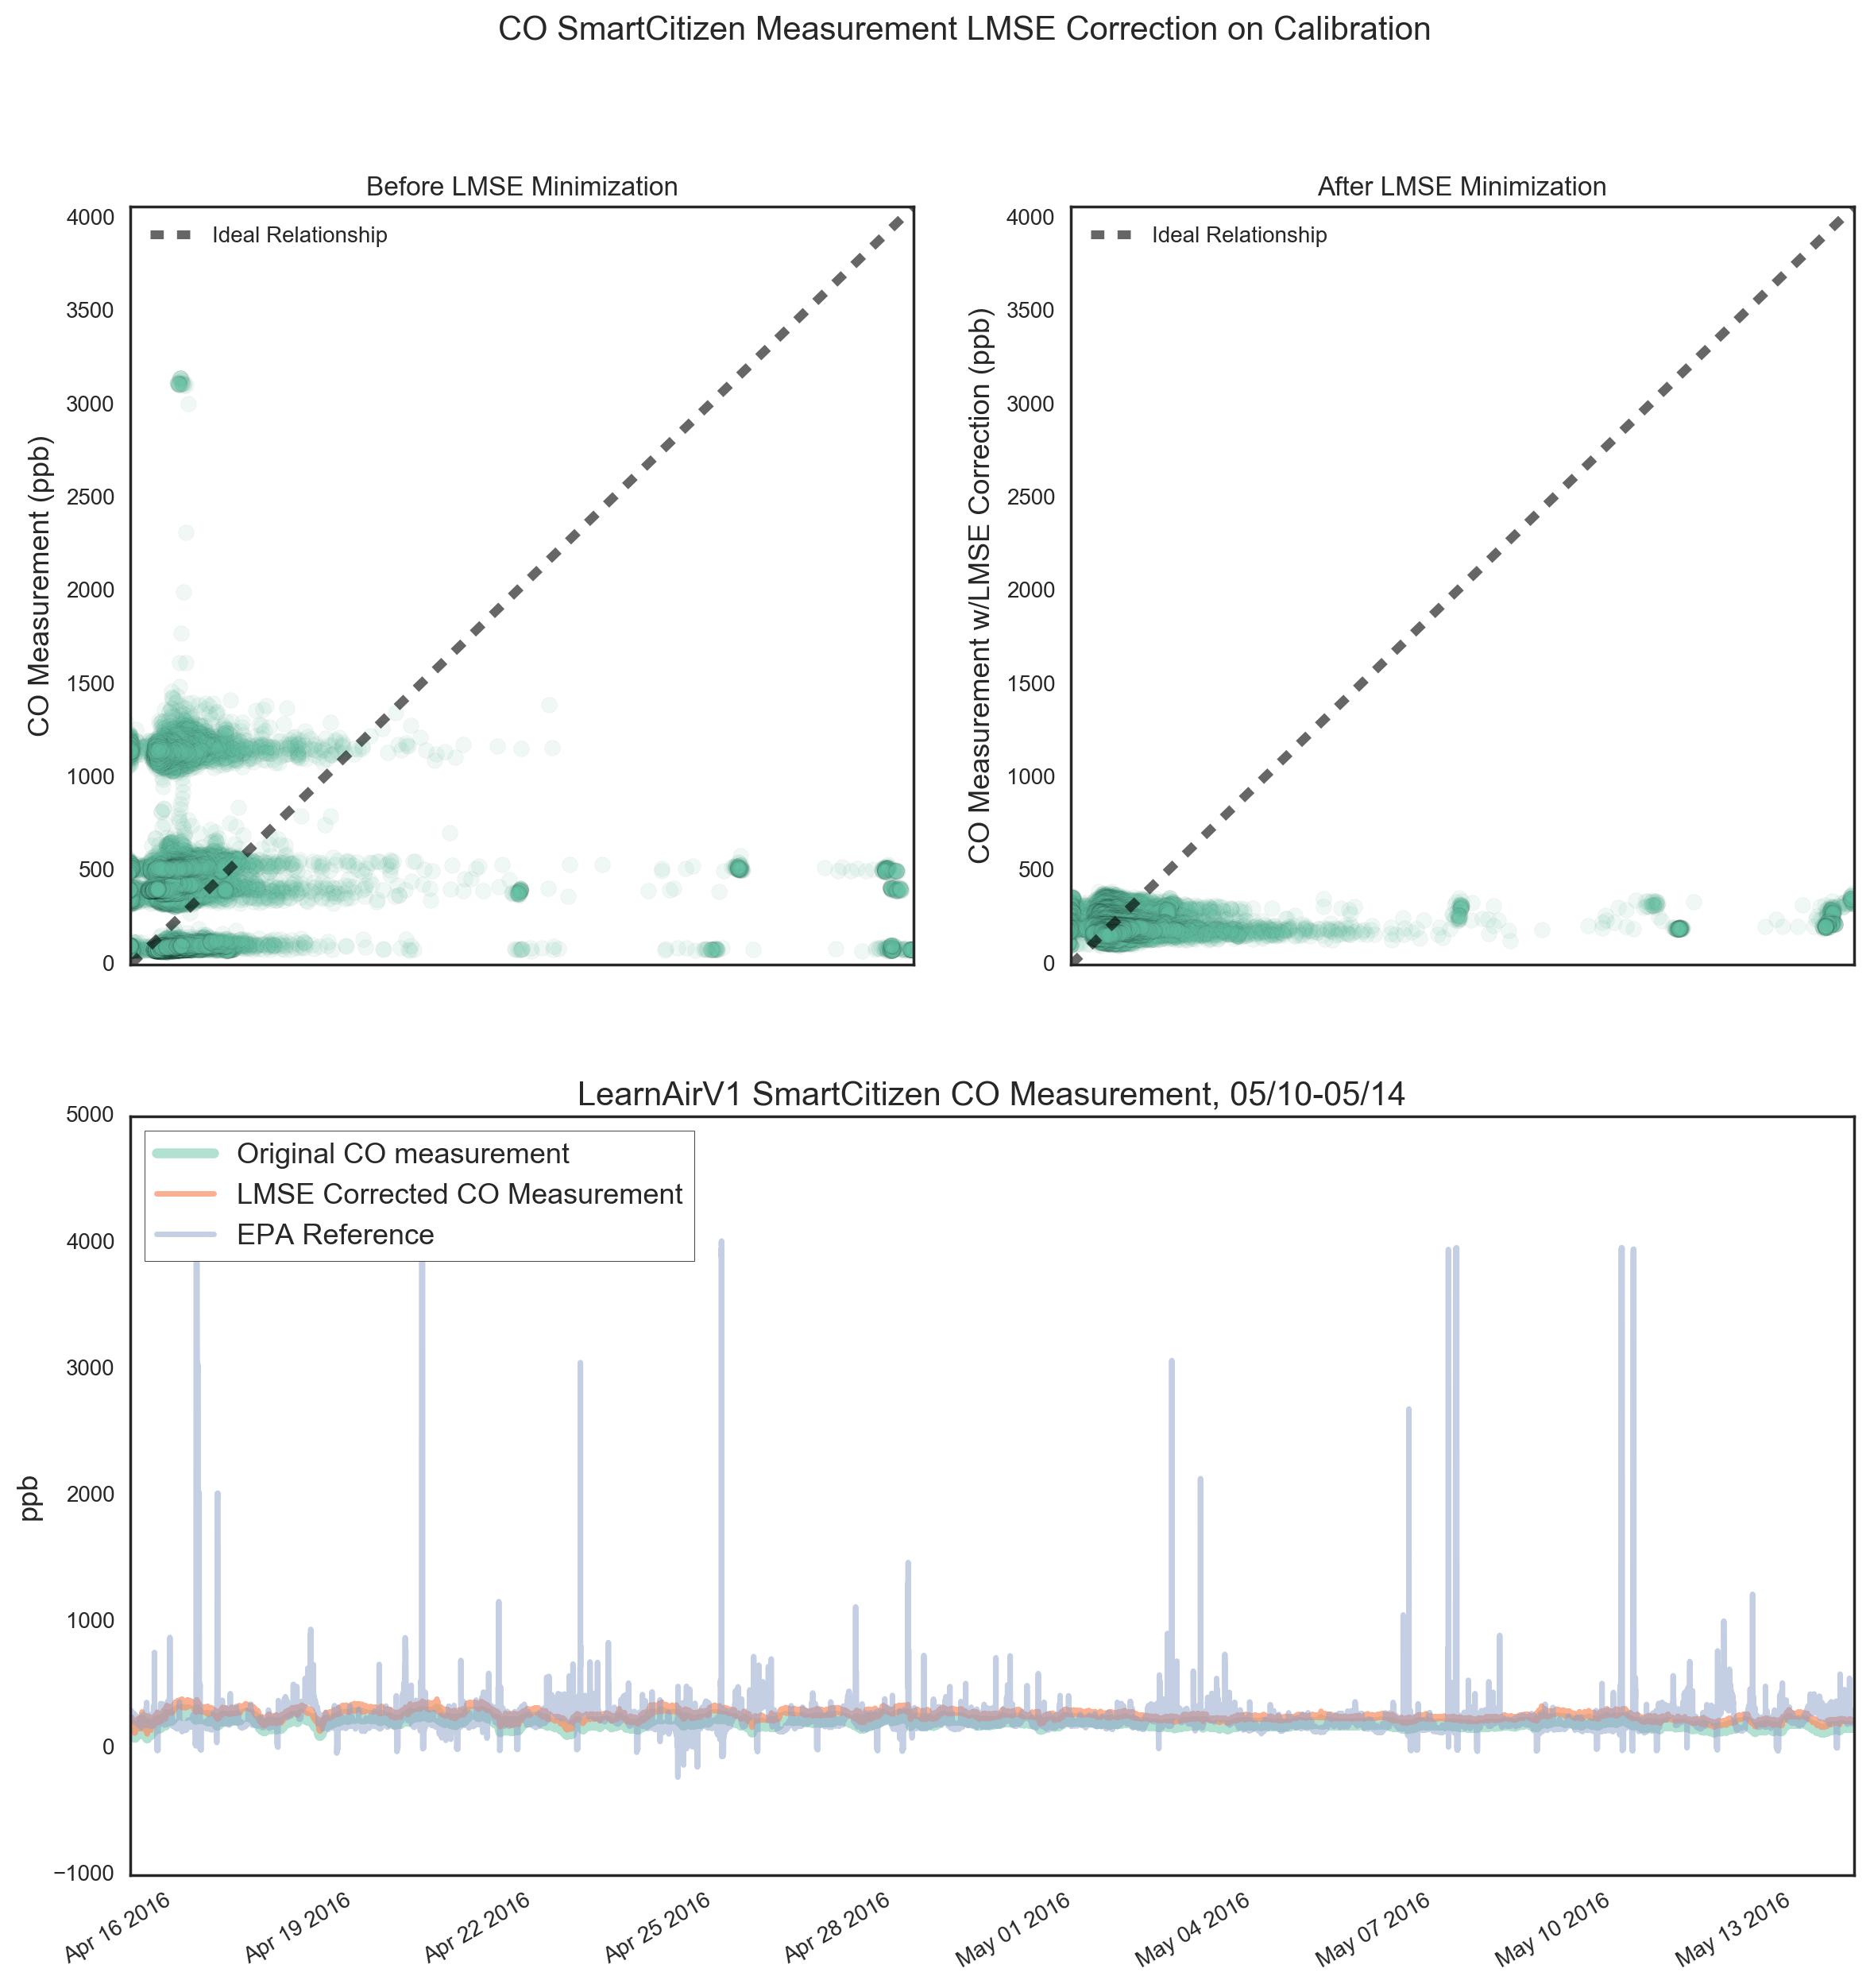
\includegraphics[width=\textwidth]{figs/sck_co_lmse}               
 	 \caption{SmartCitizen CO after LMSE Calibration}
  	\label{fig:sck_co_lmse}
\end{figure}

\begin{figure}[htb]
 	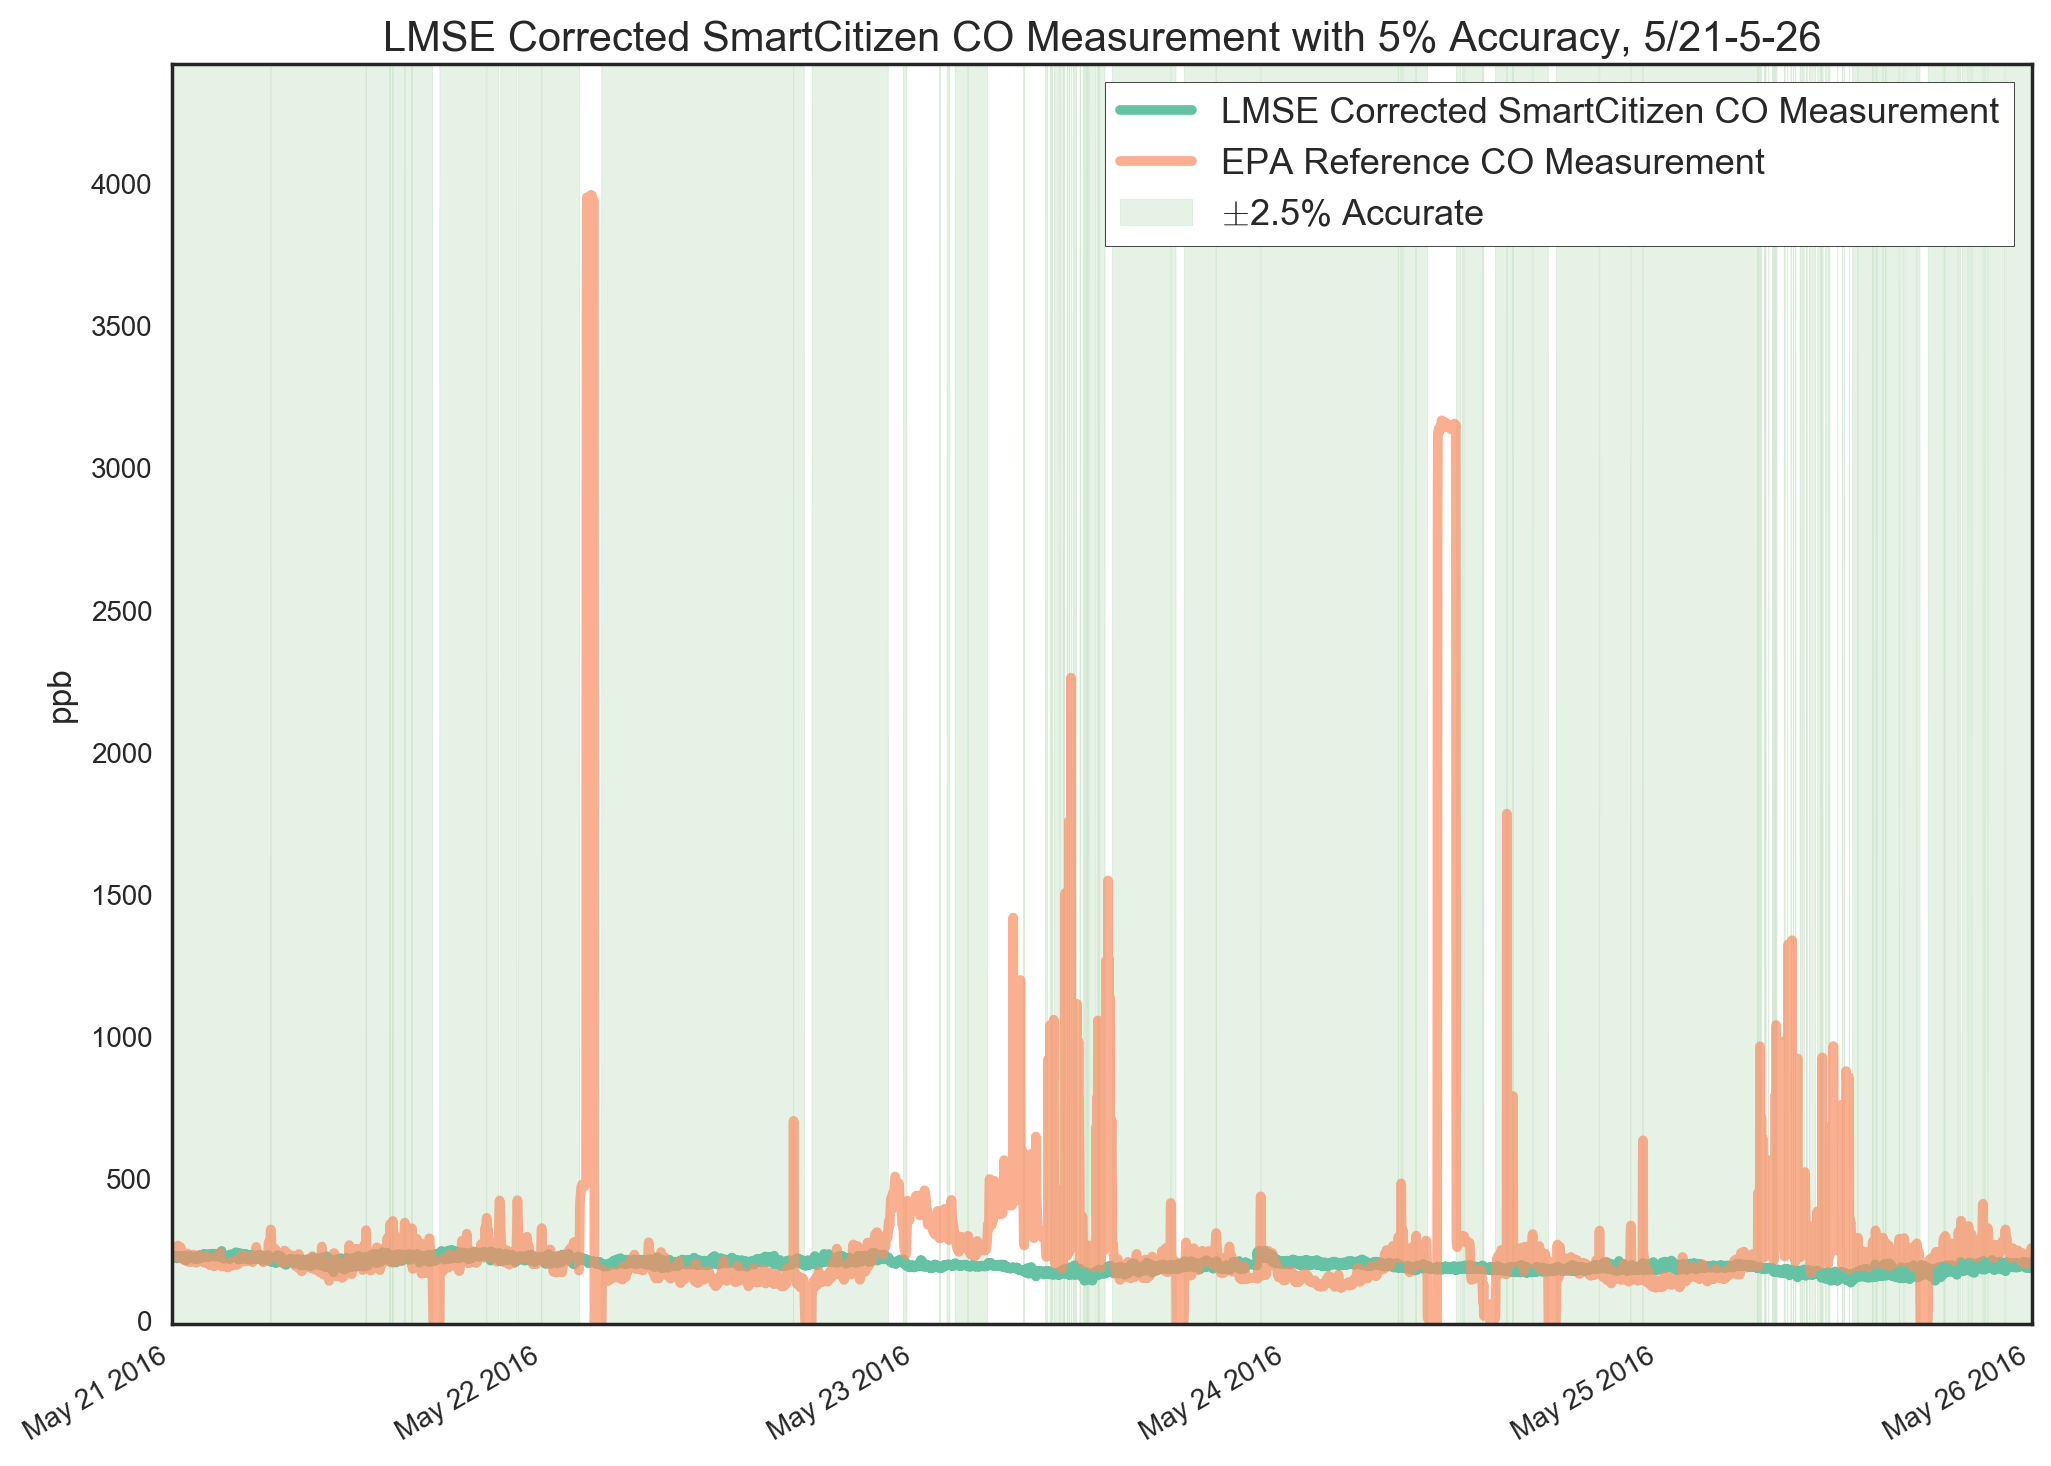
\includegraphics[width=\textwidth]{figs/sck_co_with_5_accuracy_zoomed}               
 	 \caption{SmartCitizen CO with 5\% Accuracy Threshold}
  	\label{fig:sck_co_with_5_accuracy_zoomed}
\end{figure}

\begin{figure}[htb]
 	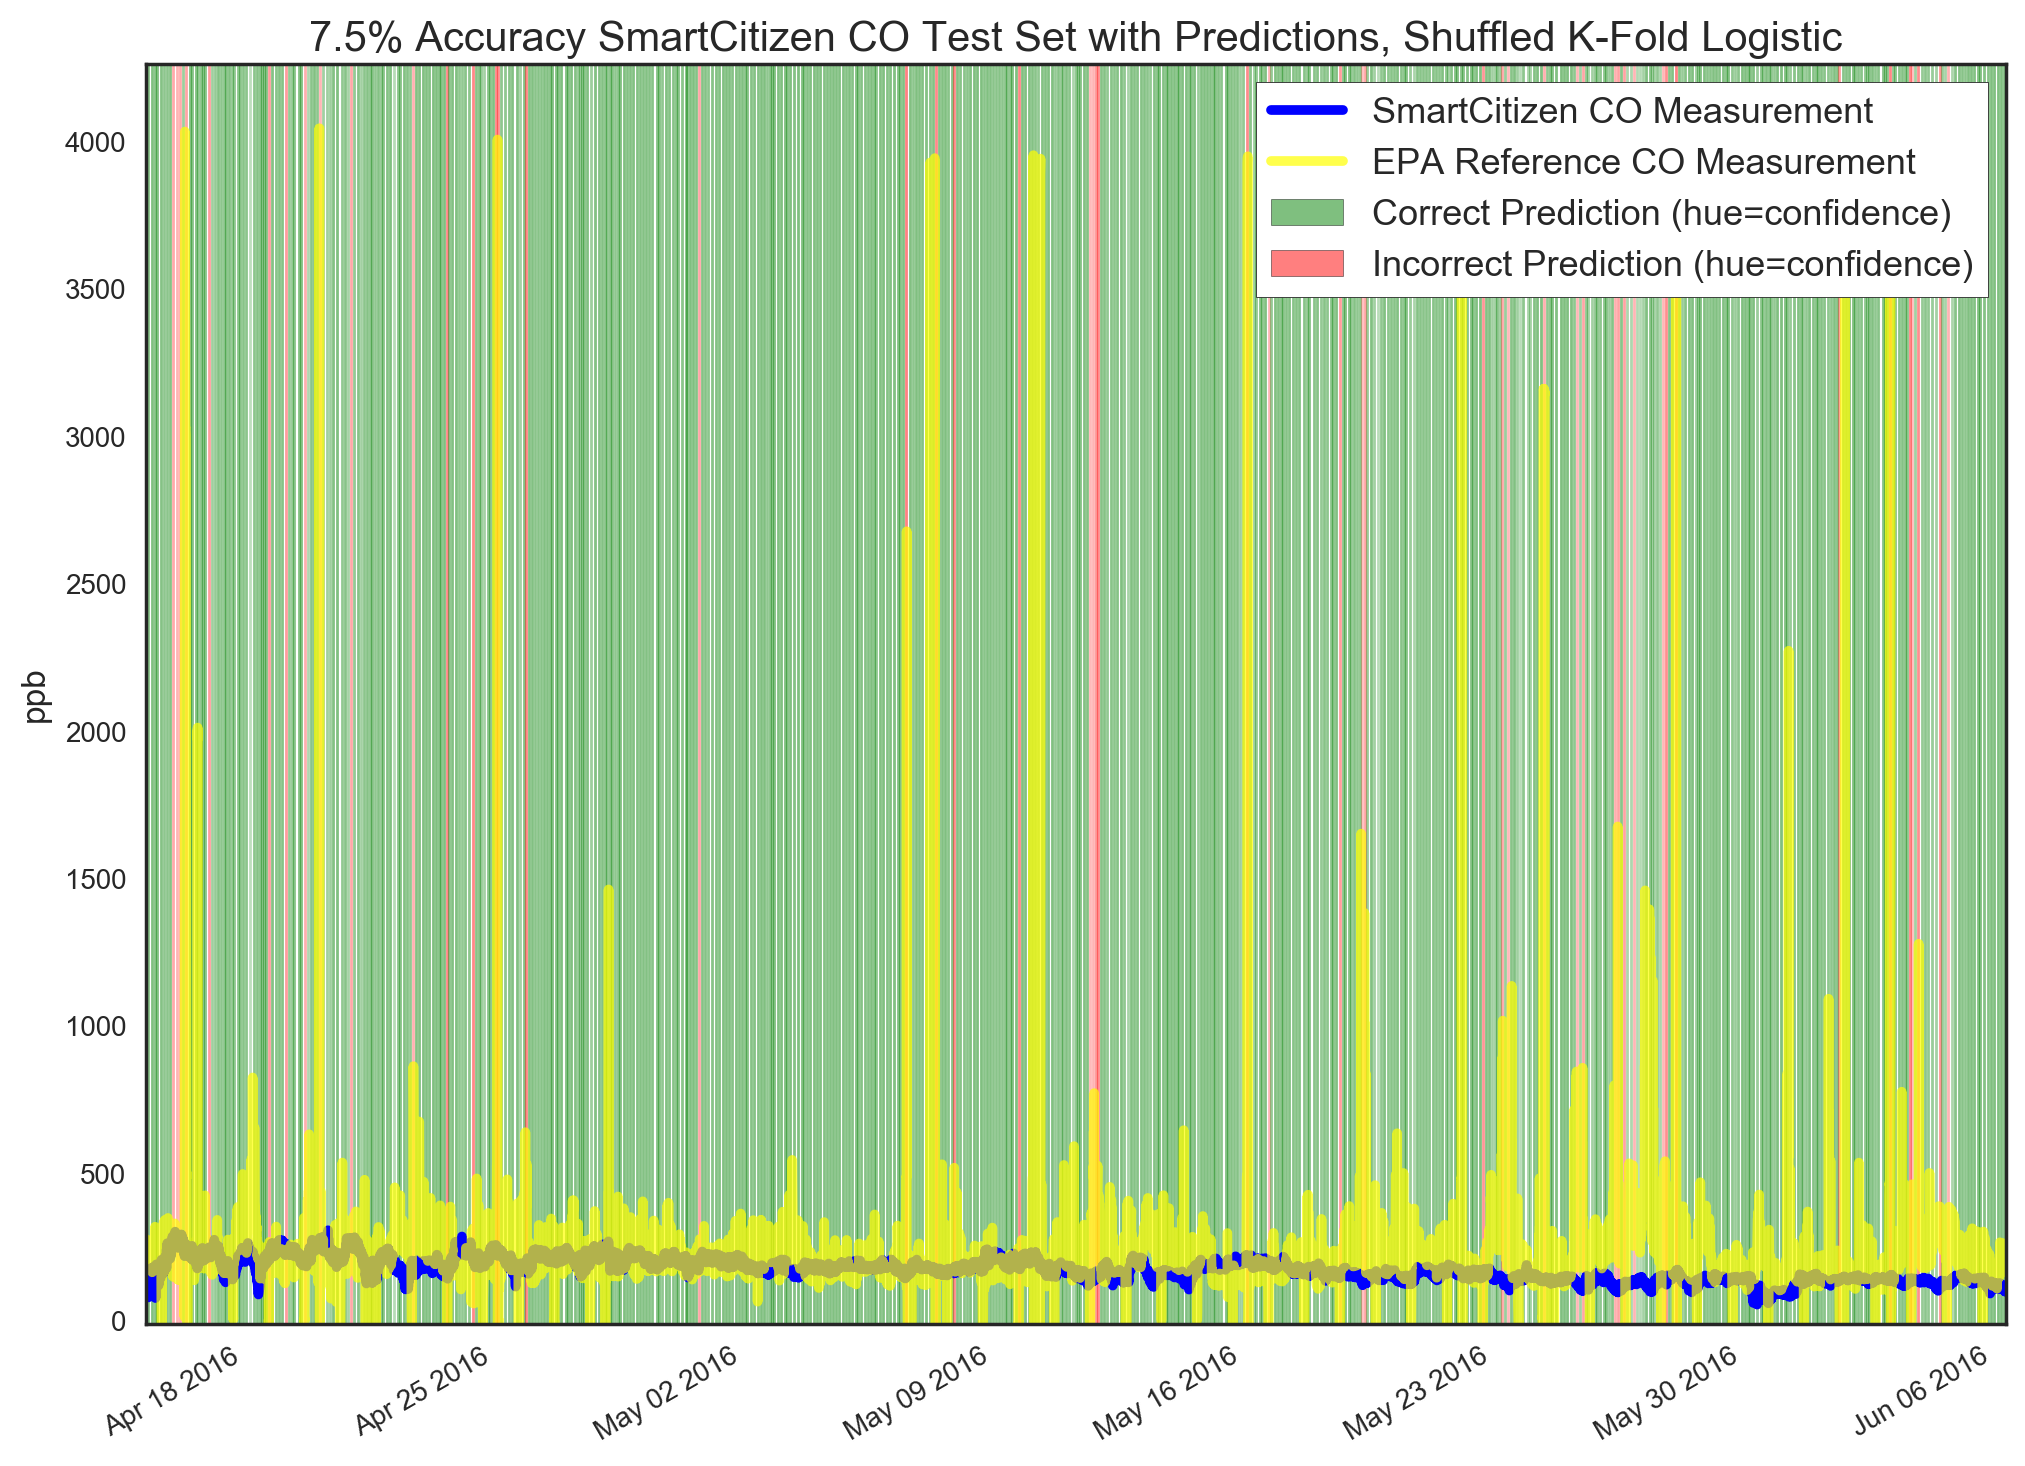
\includegraphics[width=\textwidth]{figs/sck_co_7p5_logistic_predictions}               
 	 \caption{SmartCitizen CO Prediction Accuracy}
  	\label{fig:sck_co_7p5_logistic_predictions}
\end{figure}

here's text referencing the (Table \ref{tab:as1_co_randomforest_features}).

\begin{table}[H]
\centering
\begin{tabular}{lllllllll}
\\
\\
\toprule
Feature & Importance \\
\midrule
bkcarbon &  0.027481618644 \\
avg\_60\_bkcarbon &  0.0265308524121 \\
avg\_720\_bkcarbon &  0.0231734007362 \\
avg\_1440\_bkcarbon &  0.0213230536622 \\
avg\_60\_forecastio\_windSpeed &  0.0155772873357 \\
min\_since\_plugged\_in &  0.0151174982516 \\
temp\_sck\_box\_differential &  0.0148499597107 \\
avg\_60\_forecastio\_windBearing &  0.014573874136 \\
daily\_avg\_forecastio\_humidity &  0.0145367615821 \\
avg\_60\_forecastio\_dewPoint &  0.0138511147354 \\
avg\_60\_forecastio\_pressure &  0.0138476329536 \\
daily\_avg\_sck\_temperature &  0.0138353139286 \\
avg\_30\_ws &  0.0136031033823 \\
daily\_avg\_sck\_humidity &  0.0135231176757 \\
avg\_720\_lmse\_scaled\_sharpDust &  0.0132885608127 \\
\bottomrule
\end{tabular}
\label{tab:as1_co_randomforest_features}
\caption{Top 15 Features from Random Forest for SmartCitizen CO, used in Pruned Logistic Regression}
\end{table}

\begin{figure}[htb]
 	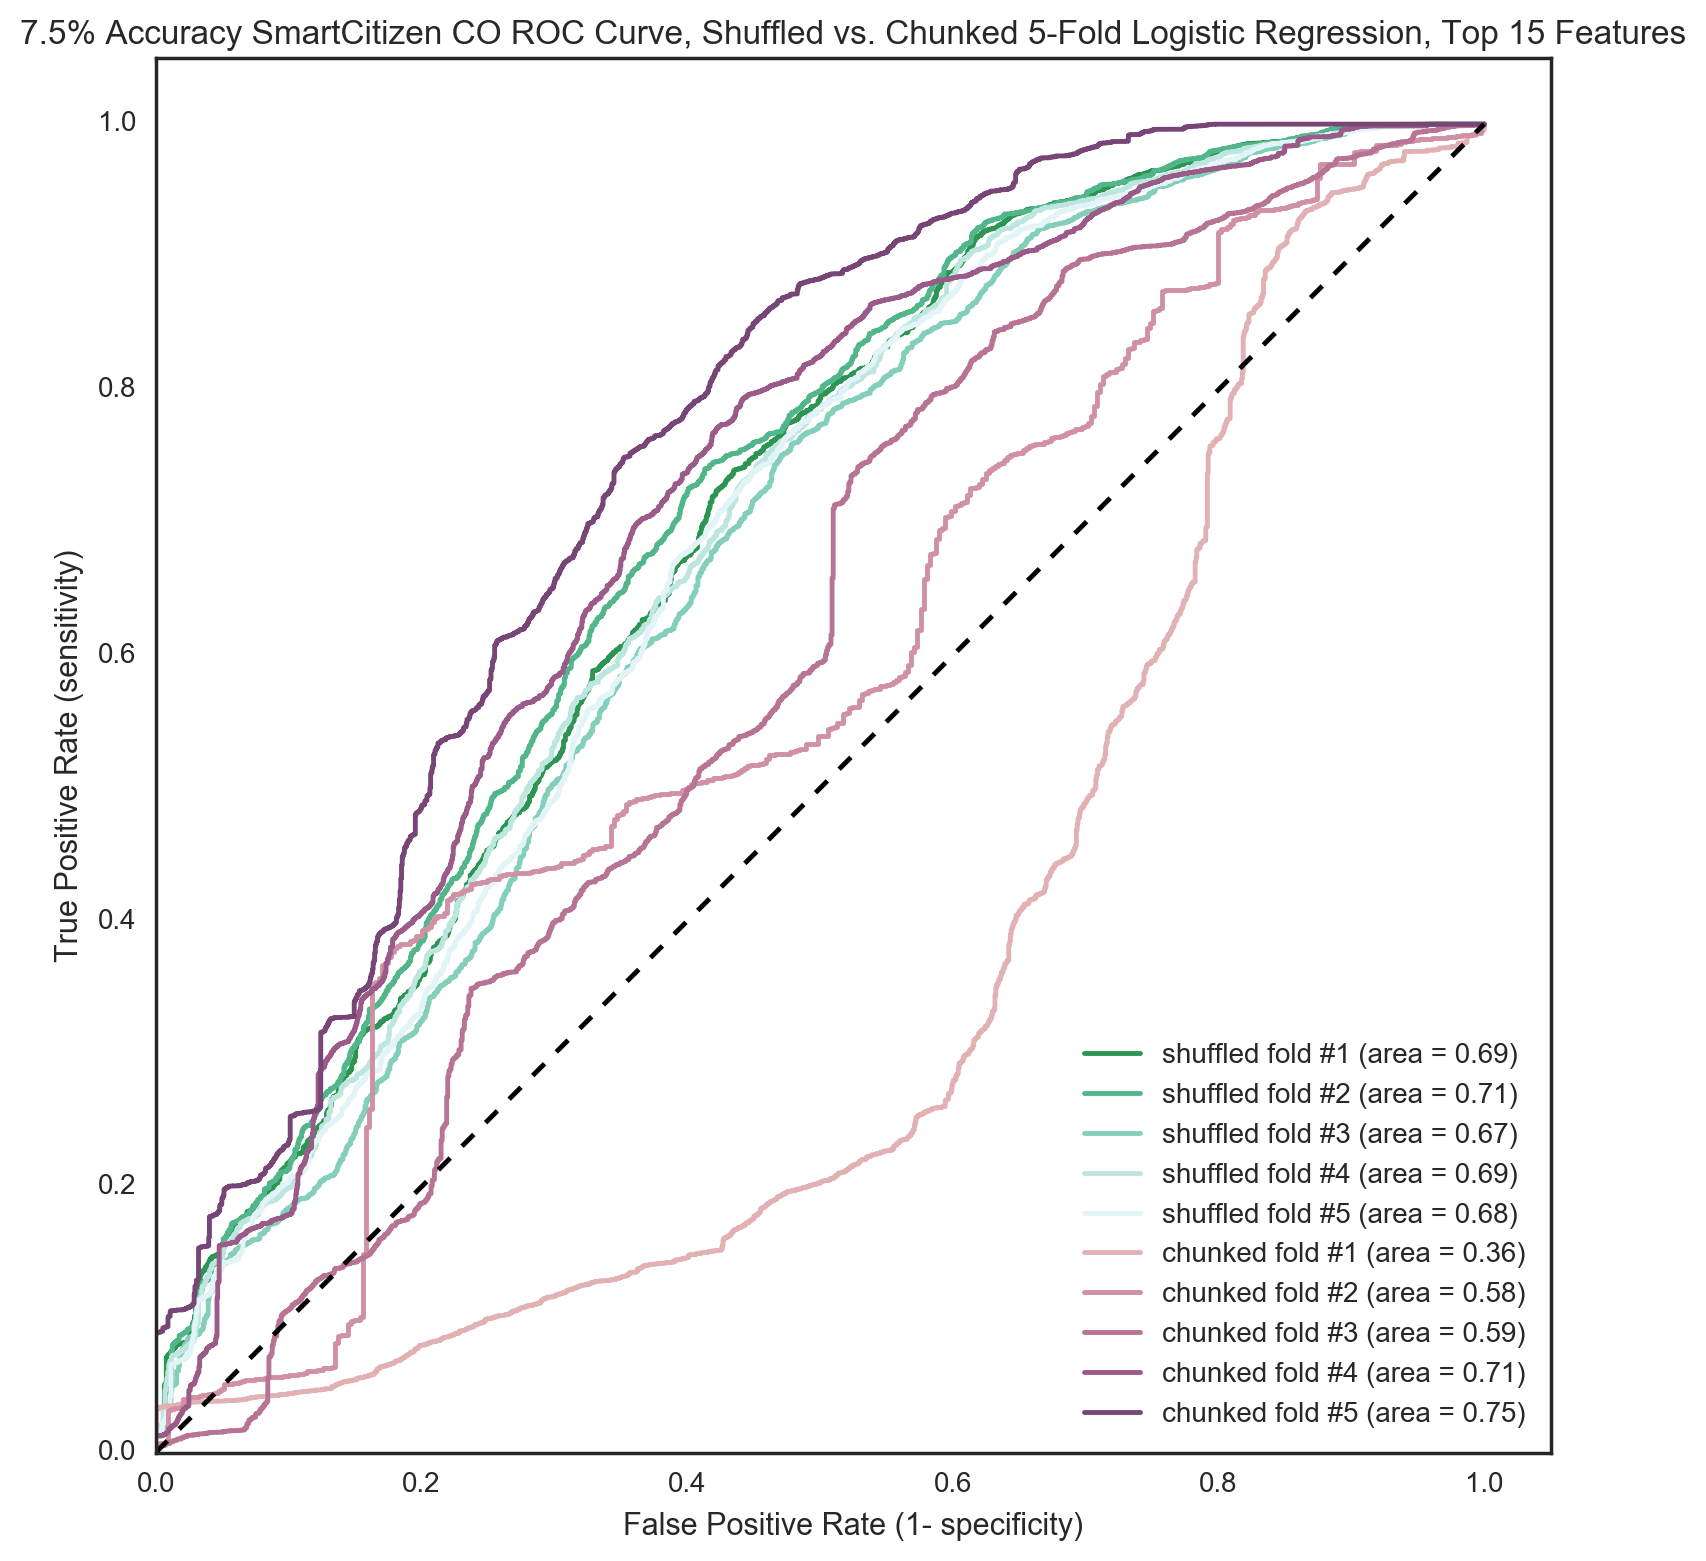
\includegraphics[width=\textwidth]{figs/sck_co_7p5_roc_pruned_features}               
 	 \caption{SmartCitizen CO ROC Using Top 15 Features}
  	\label{fig:sck_co_7p5_roc_pruned_features}
\end{figure}

\FloatBarrier
\section{SmartCitizen NO2}
\FloatBarrier

\begin{figure}[htb]
 	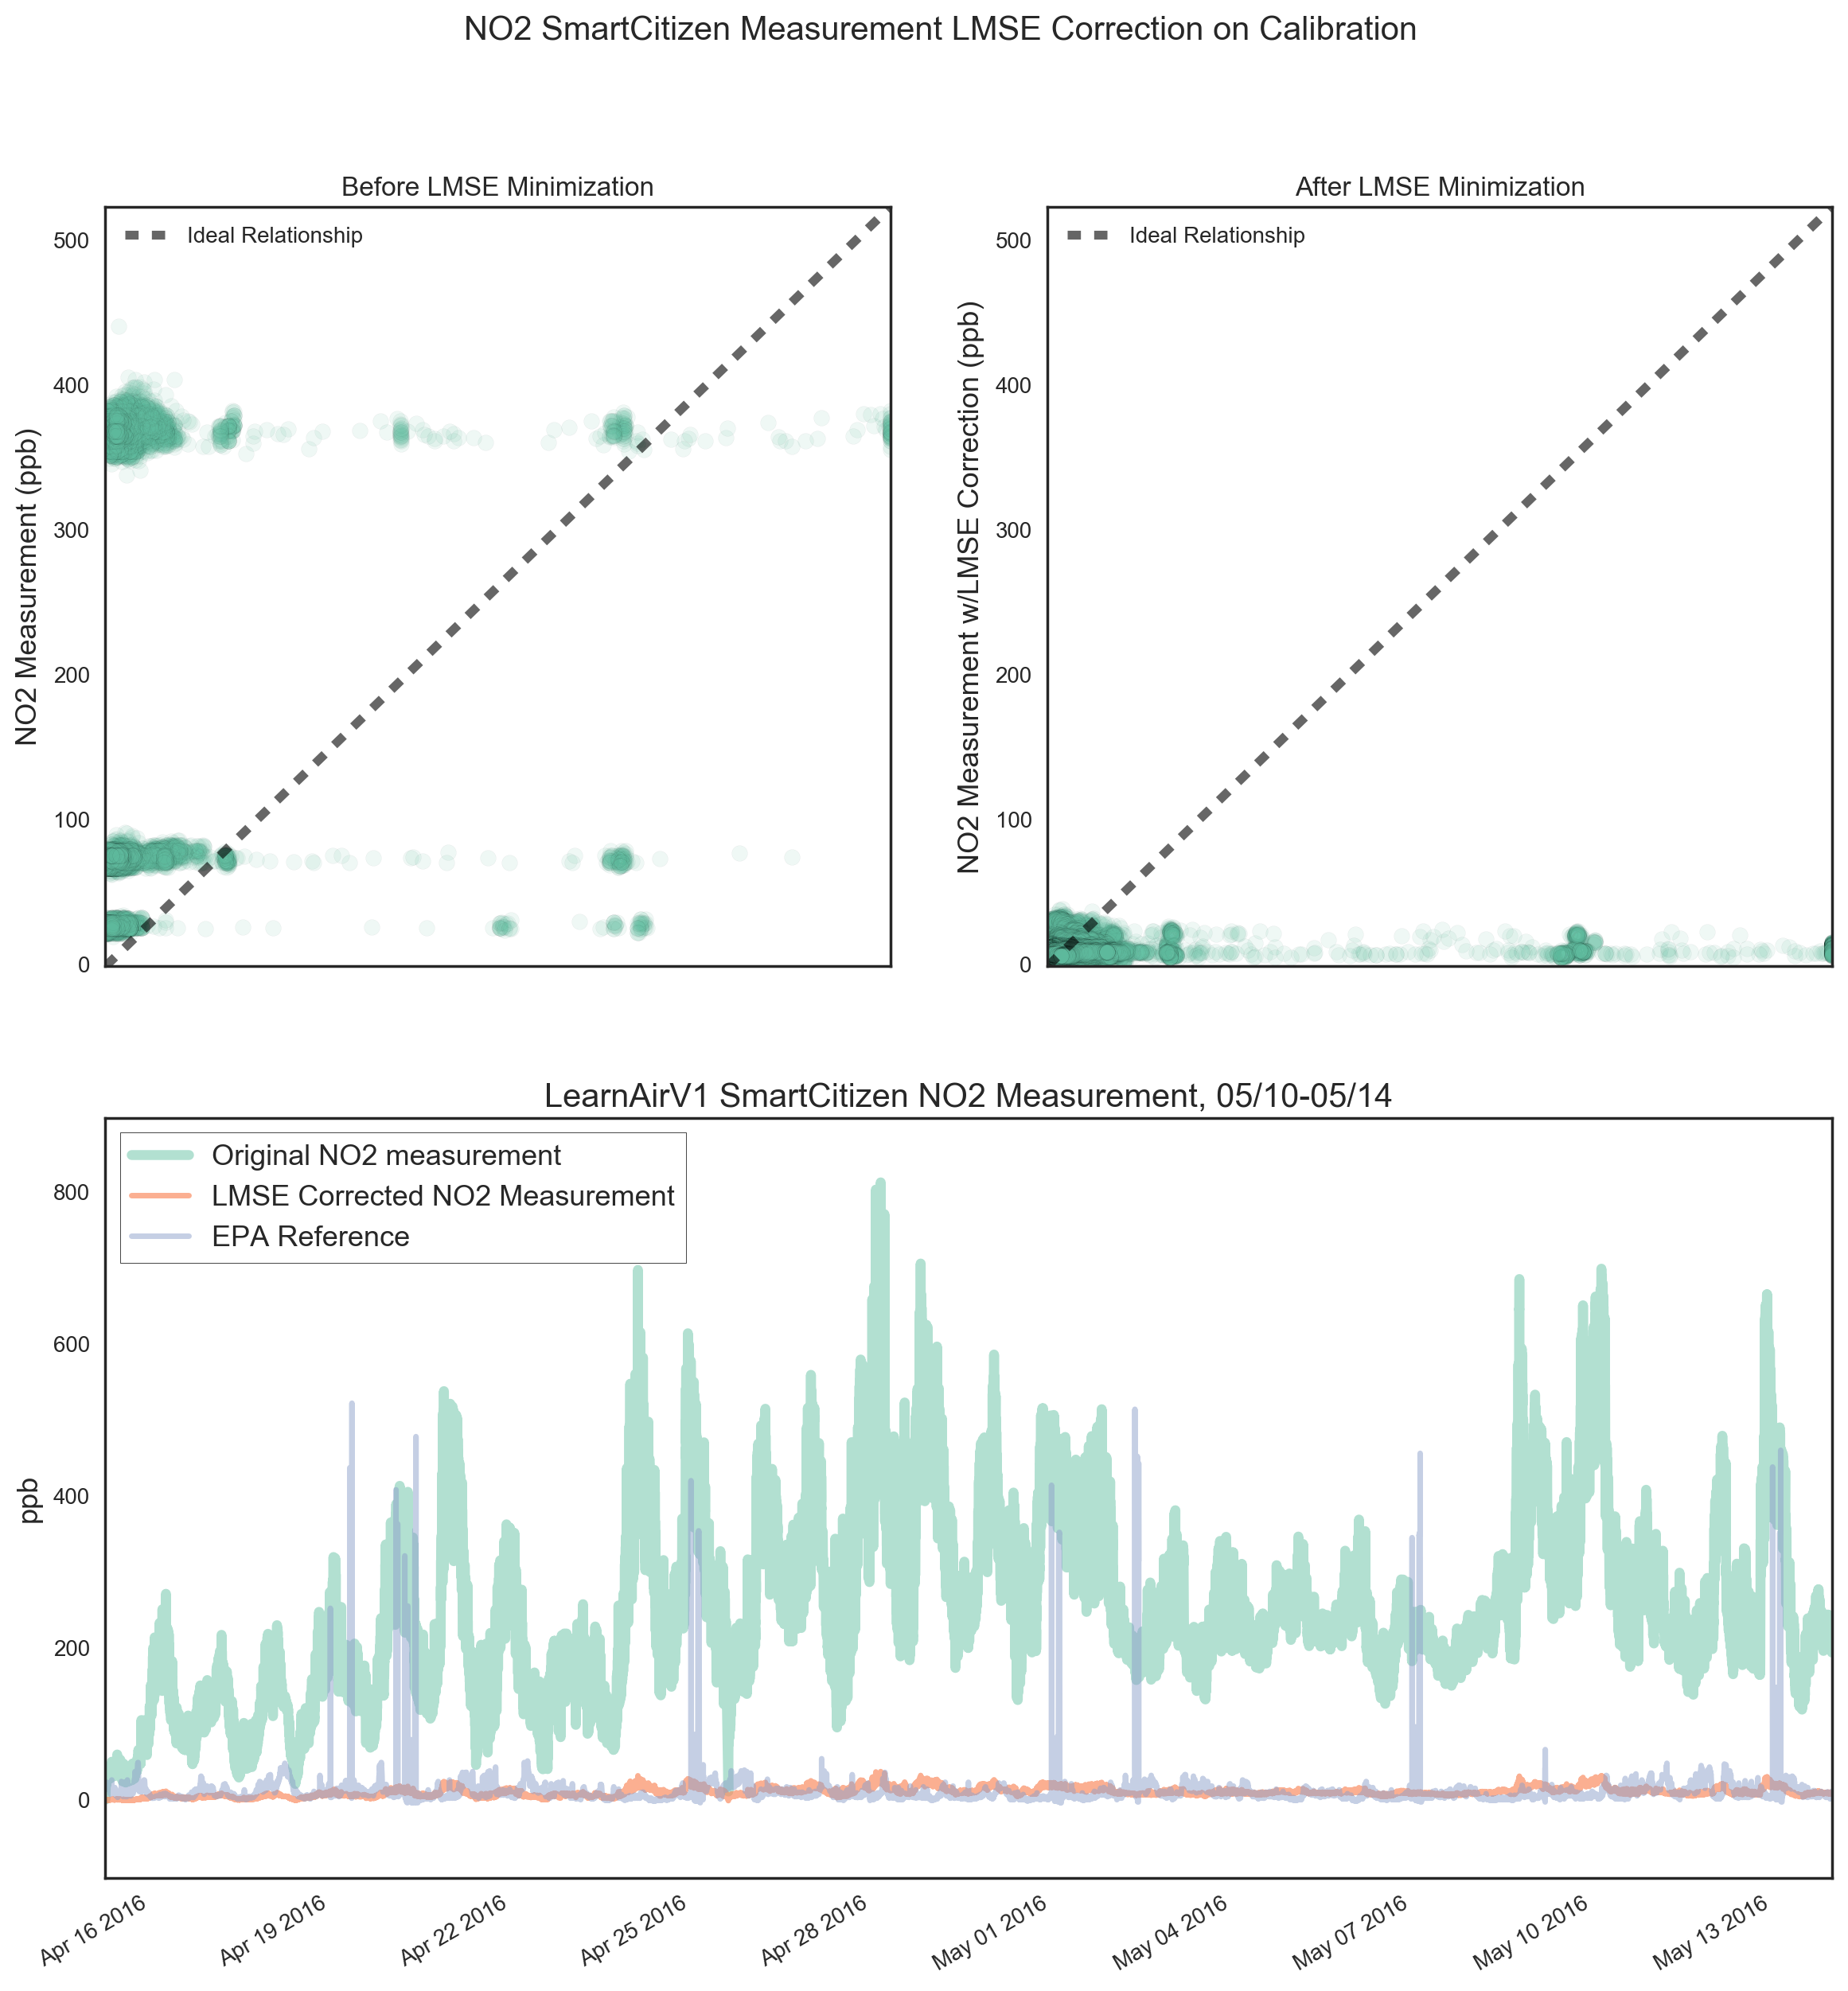
\includegraphics[width=\textwidth]{figs/sck_no2_lmse}               
 	 \caption{SmartCitizen NO2 after LMSE Calibration}
  	\label{fig:sck_no2_lmse}
\end{figure}

\begin{figure}[htb]
 	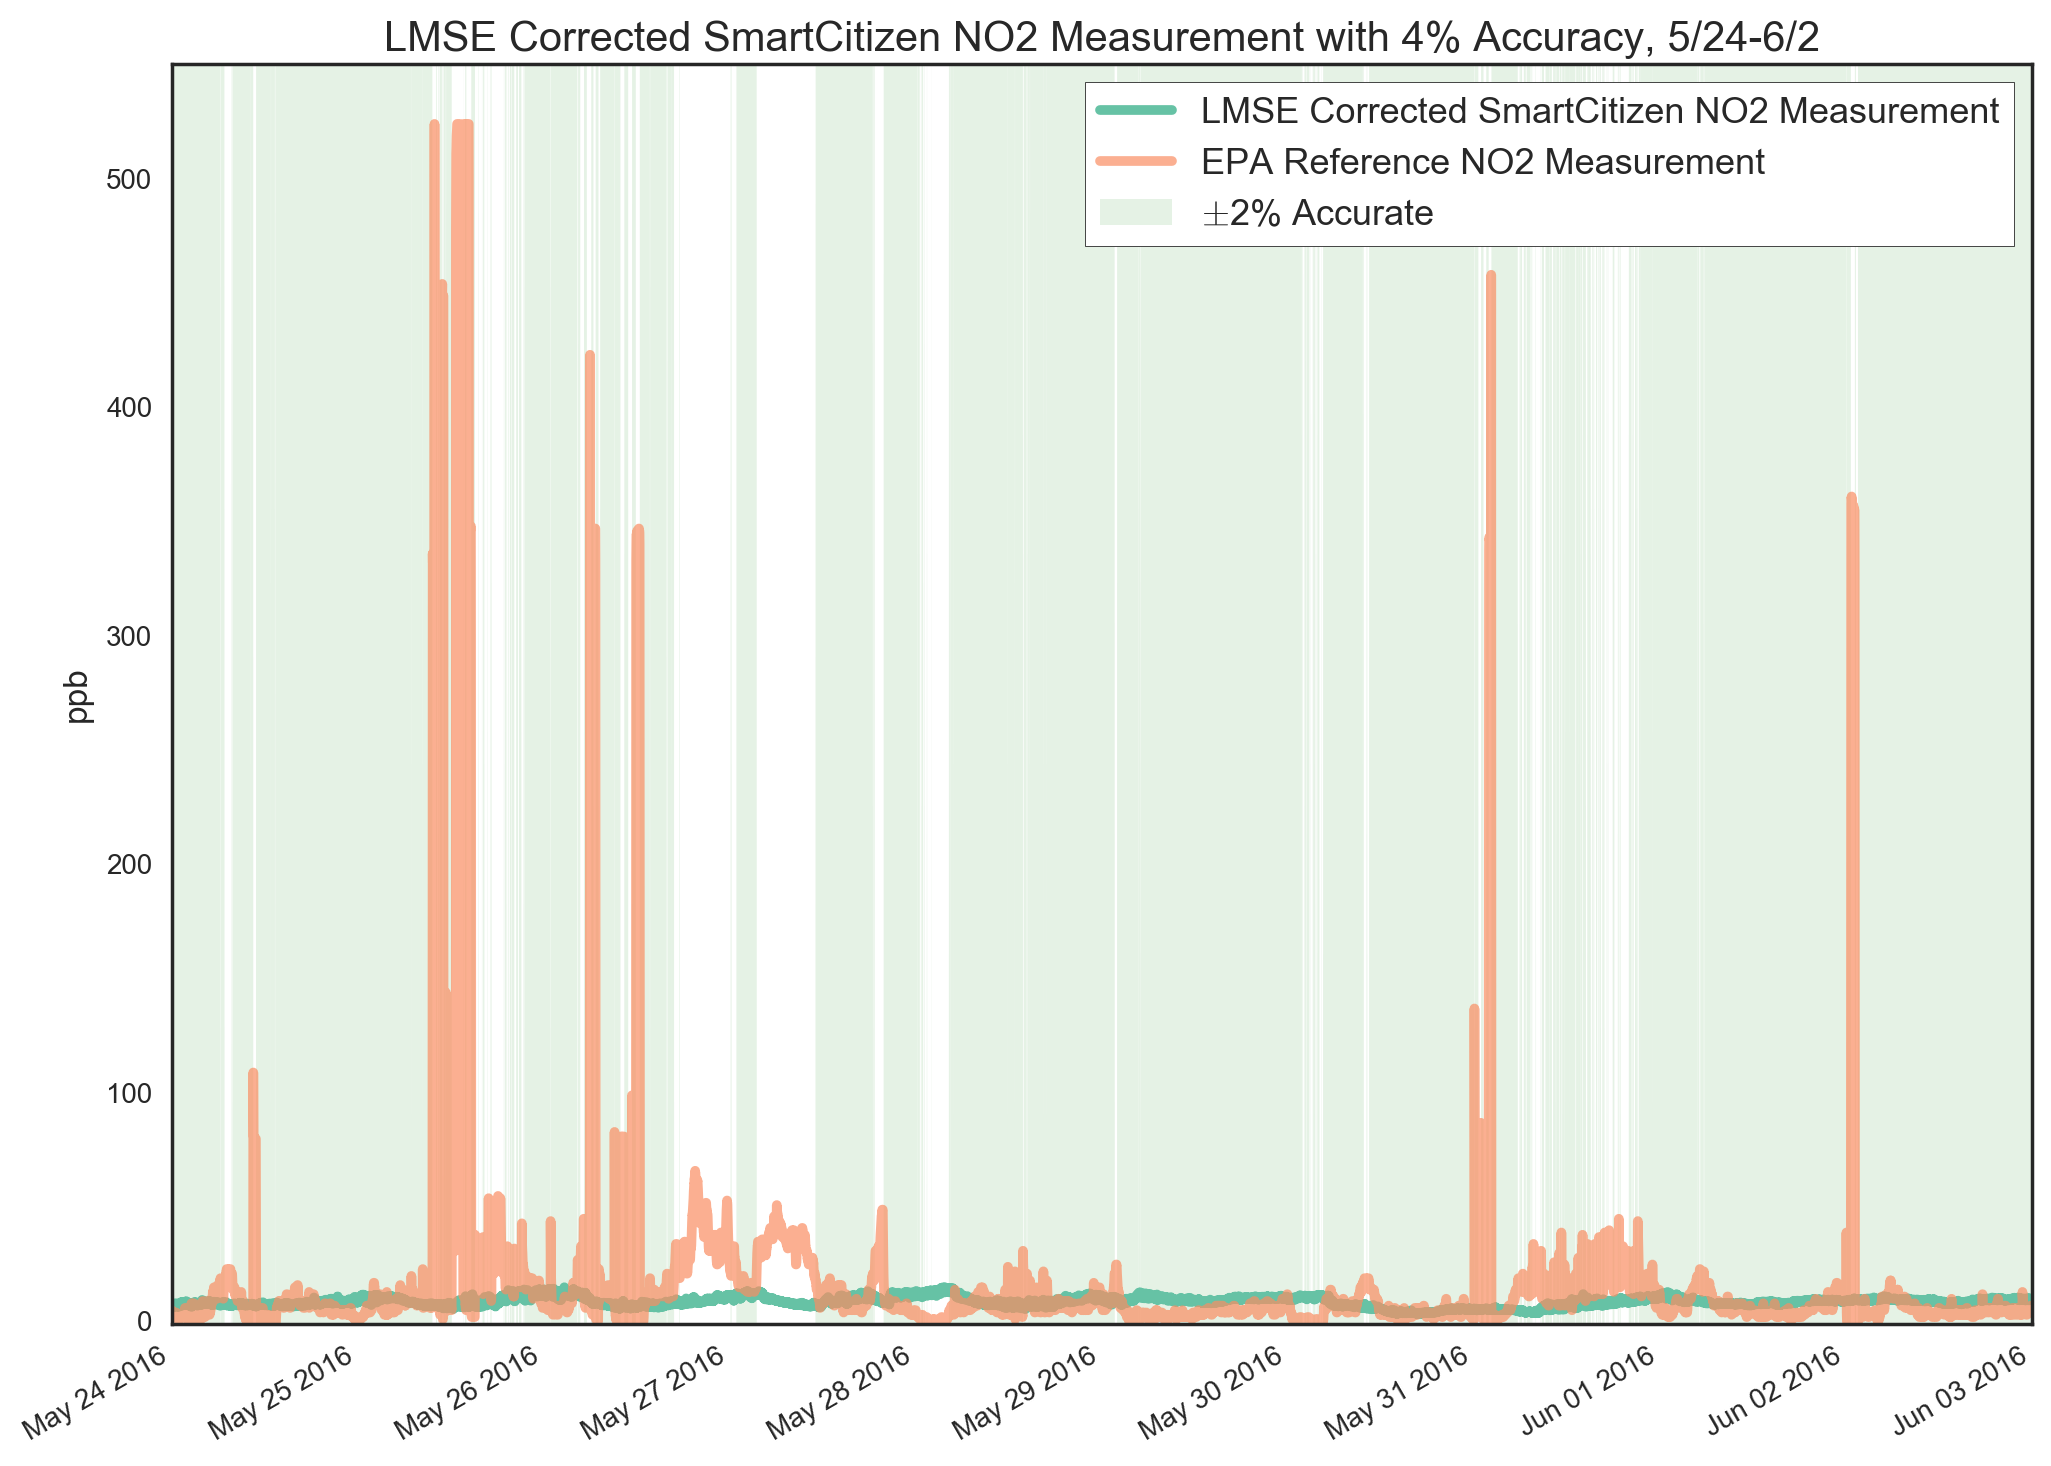
\includegraphics[width=\textwidth]{figs/sck_no2_with_4_accuracy_zoomed}               
 	 \caption{SmartCitizen NO2 with 4\% Accuracy Threshold}
  	\label{fig:sck_no2_with_4_accuracy_zoomed}
\end{figure}

\begin{figure}[htb]
 	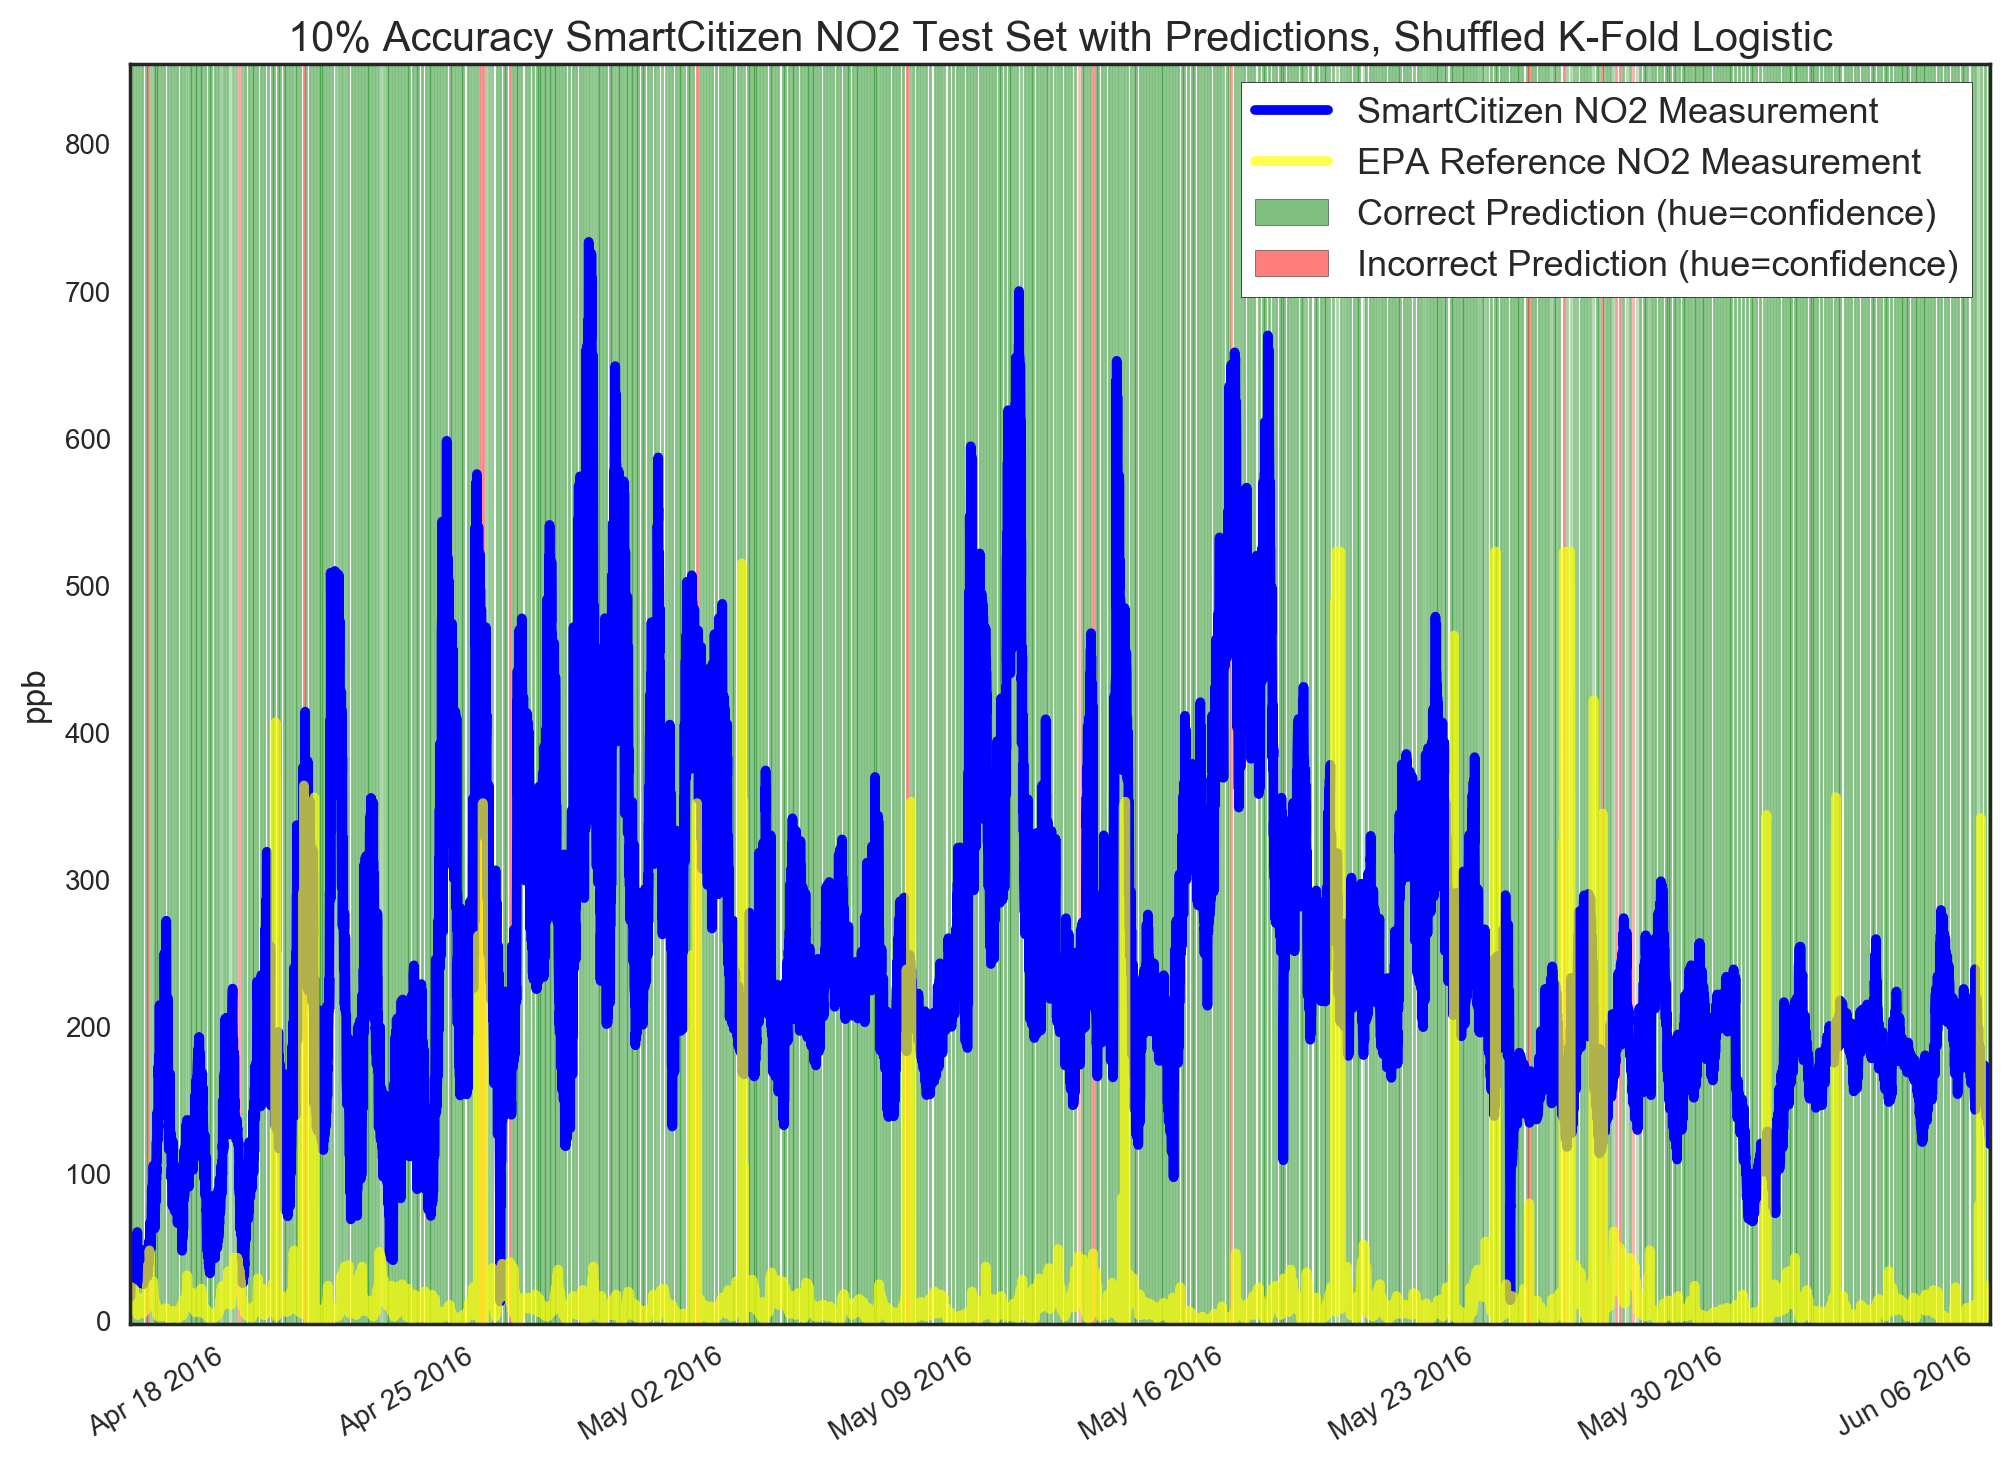
\includegraphics[width=\textwidth]{figs/sck_no2_10_logistic_predictions}               
 	 \caption{SmartCitizen NO2 Prediction Accuracy}
  	\label{fig:sck_no2_10_logistic_predictions}
\end{figure}

here's text referencing the (Table \ref{tab:sck_no2_randomforest_features}).

\begin{table}[H]
\centering
\begin{tabular}{lllllllll}
\\
\\
\toprule
Feature & Importance \\
\midrule

bkcarbon & 0.0459890536212 \\
avg\_60\_bkcarbon & 0.0433384018273 \\
avg\_720\_bkcarbon & 0.024690468695 \\
avg\_1440\_bkcarbon & 0.0210702674105 \\
avg\_60\_forecastio\_windSpeed & 0.0207714428351 \\
min\_since\_plugged\_in & 0.0173782542533 \\
avg\_60\_forecastio\_windBearing & 0.0172875801677 \\
forecastio\_windSpeed & 0.0170176630128 \\
avg\_1440\_lmse\_calib\_as\_co & 0.0162266191466 \\
daily\_avg\_sck\_humidity & 0.0160827543221 \\
avg\_60\_forecastio\_pressure & 0.0157403595739 \\
avg\_720\_lmse\_scaled\_sharpDust & 0.0154263296837 \\
avg\_1440\_lmse\_scaled\_sharpDust & 0.0153038668128 \\
daily\_avg\_as\_temperature & 0.0151434934355 \\
daily\_avg\_forecastio\_temperature & 0.0148922895233 \\
\bottomrule
\end{tabular}
\label{tab:sck_no2_randomforest_features}
\caption{Top 15 Features from Random Forest for SmartCitizen NO2, used in Pruned Logistic Regression}
\end{table}

\begin{figure}[htb]
 	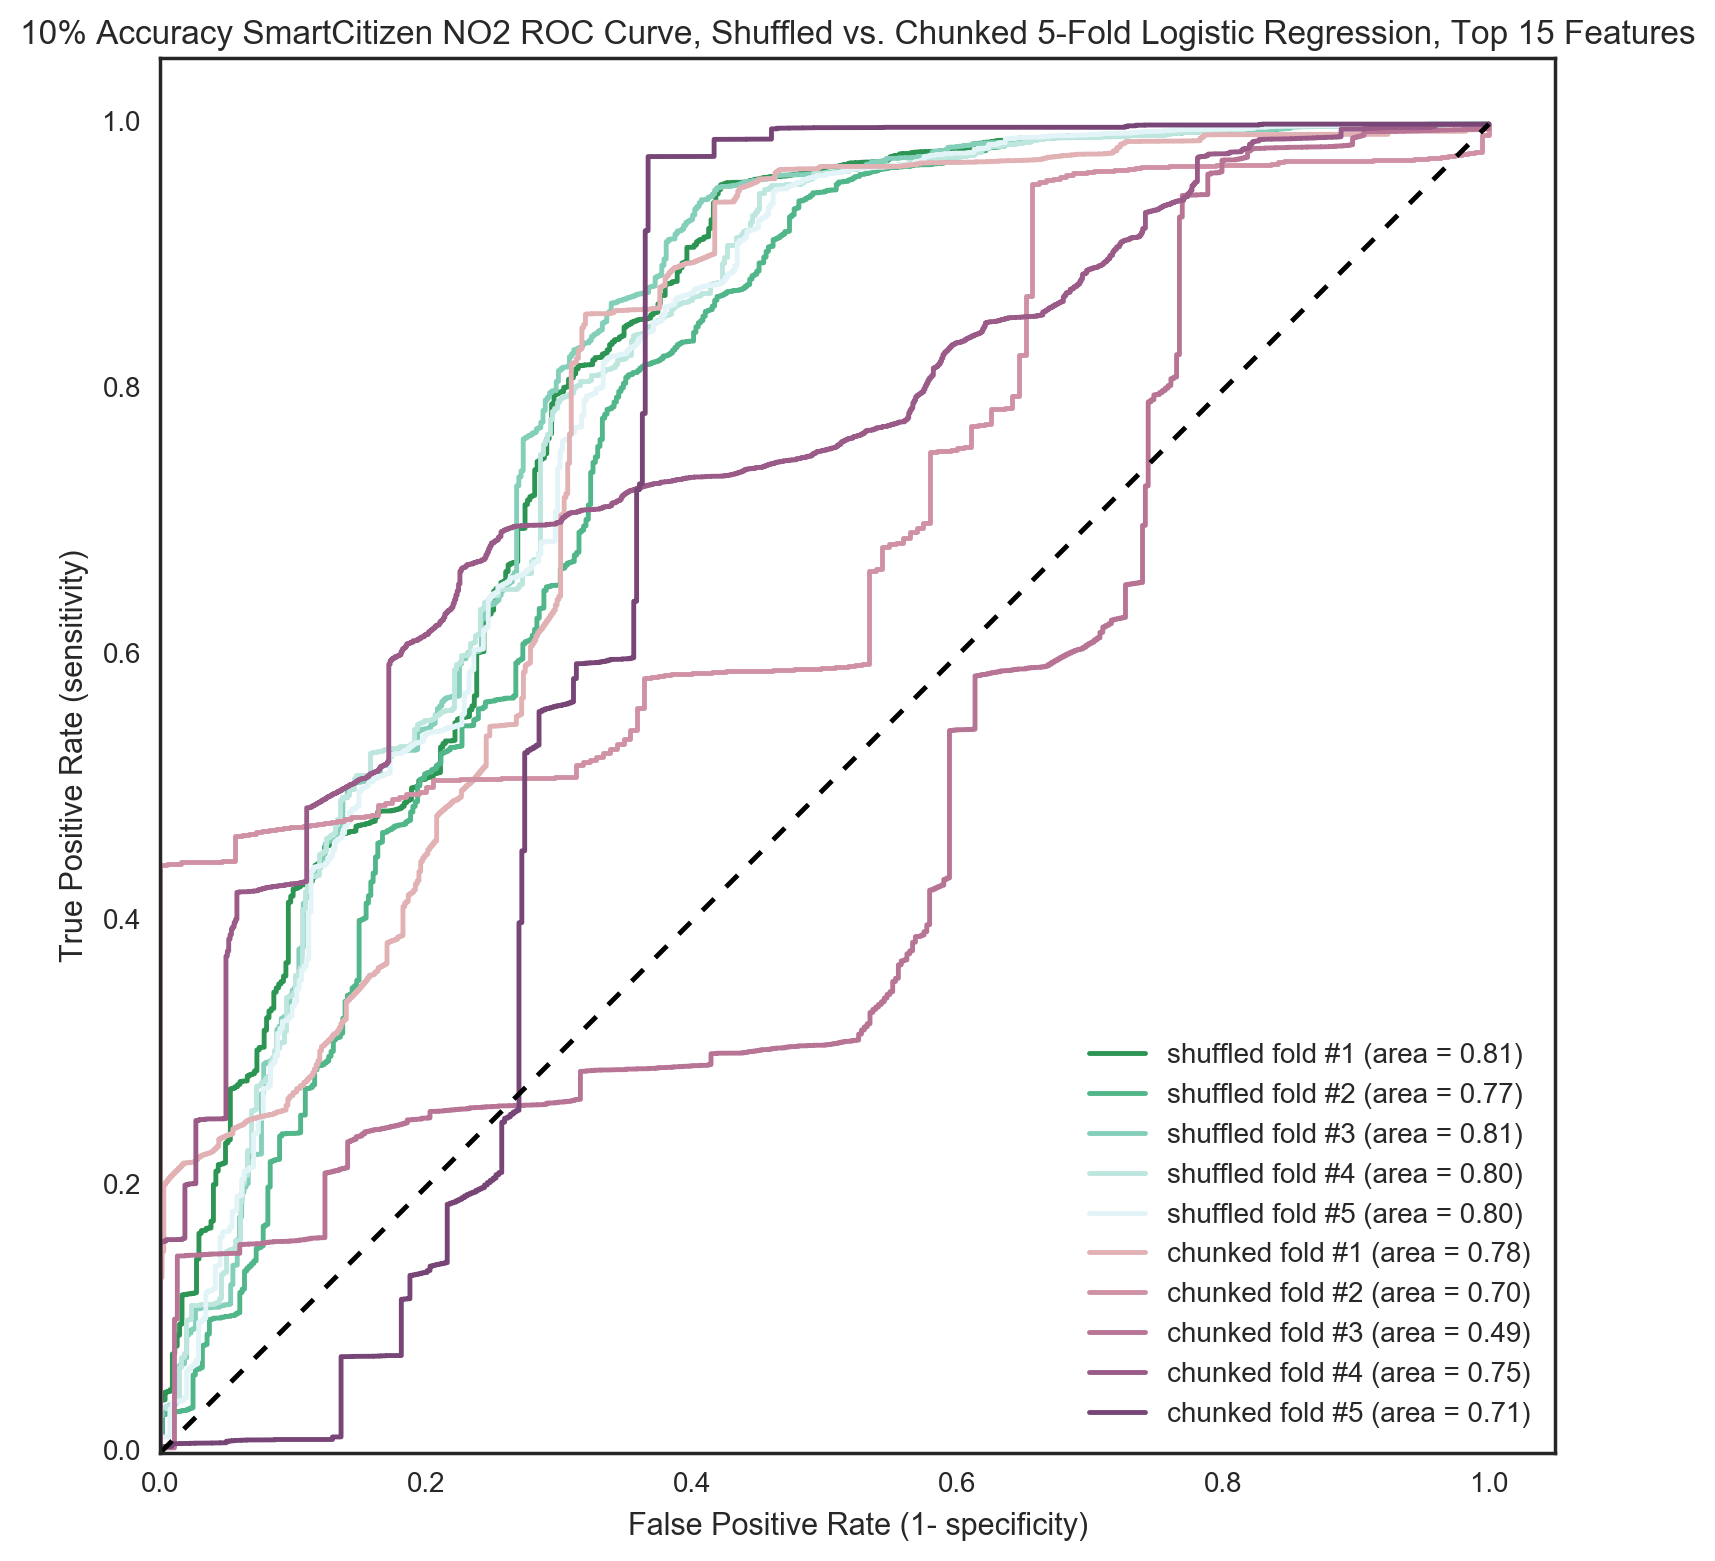
\includegraphics[width=\textwidth]{figs/sck_no2_10_roc_pruned_features}               
 	 \caption{SmartCitizen NO2 ROC Using Top 15 Features}
  	\label{fig:sck_no2_10_roc_pruned_features}
\end{figure}


\FloatBarrier
\section{Sharp Dust Sensor}
\FloatBarrier

\begin{figure}[htb]
 	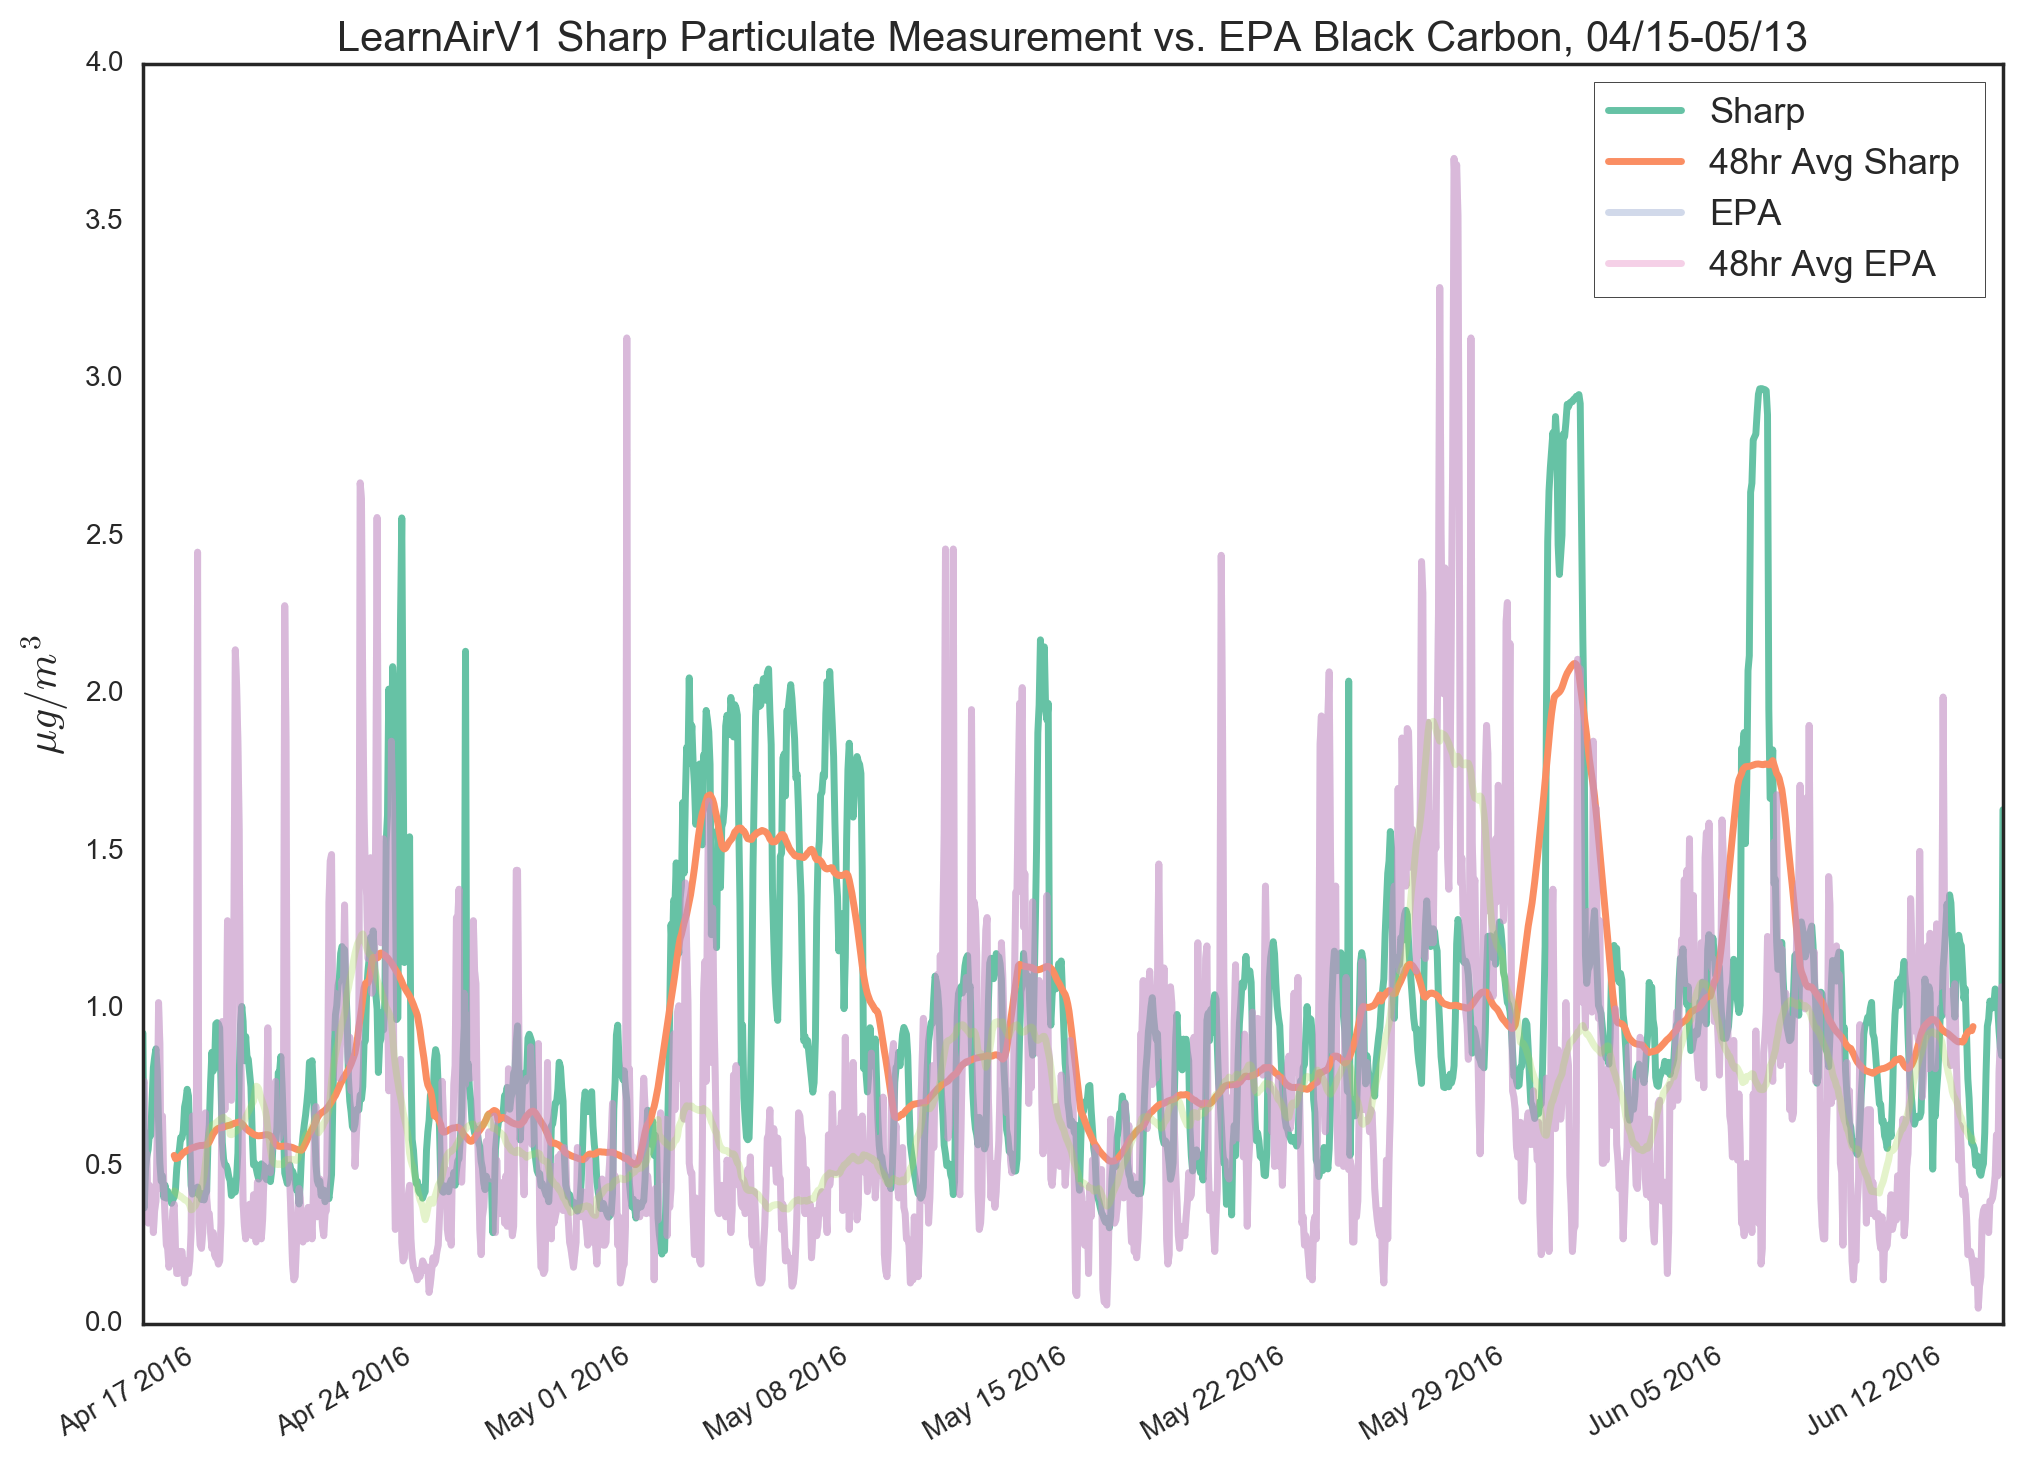
\includegraphics[width=\textwidth]{figs/sharp_raw}               
 	 \caption{Sharp Raw Particulate Data}
  	\label{fig:sharp_raw}
\end{figure}


\begin{figure}[htb]
 	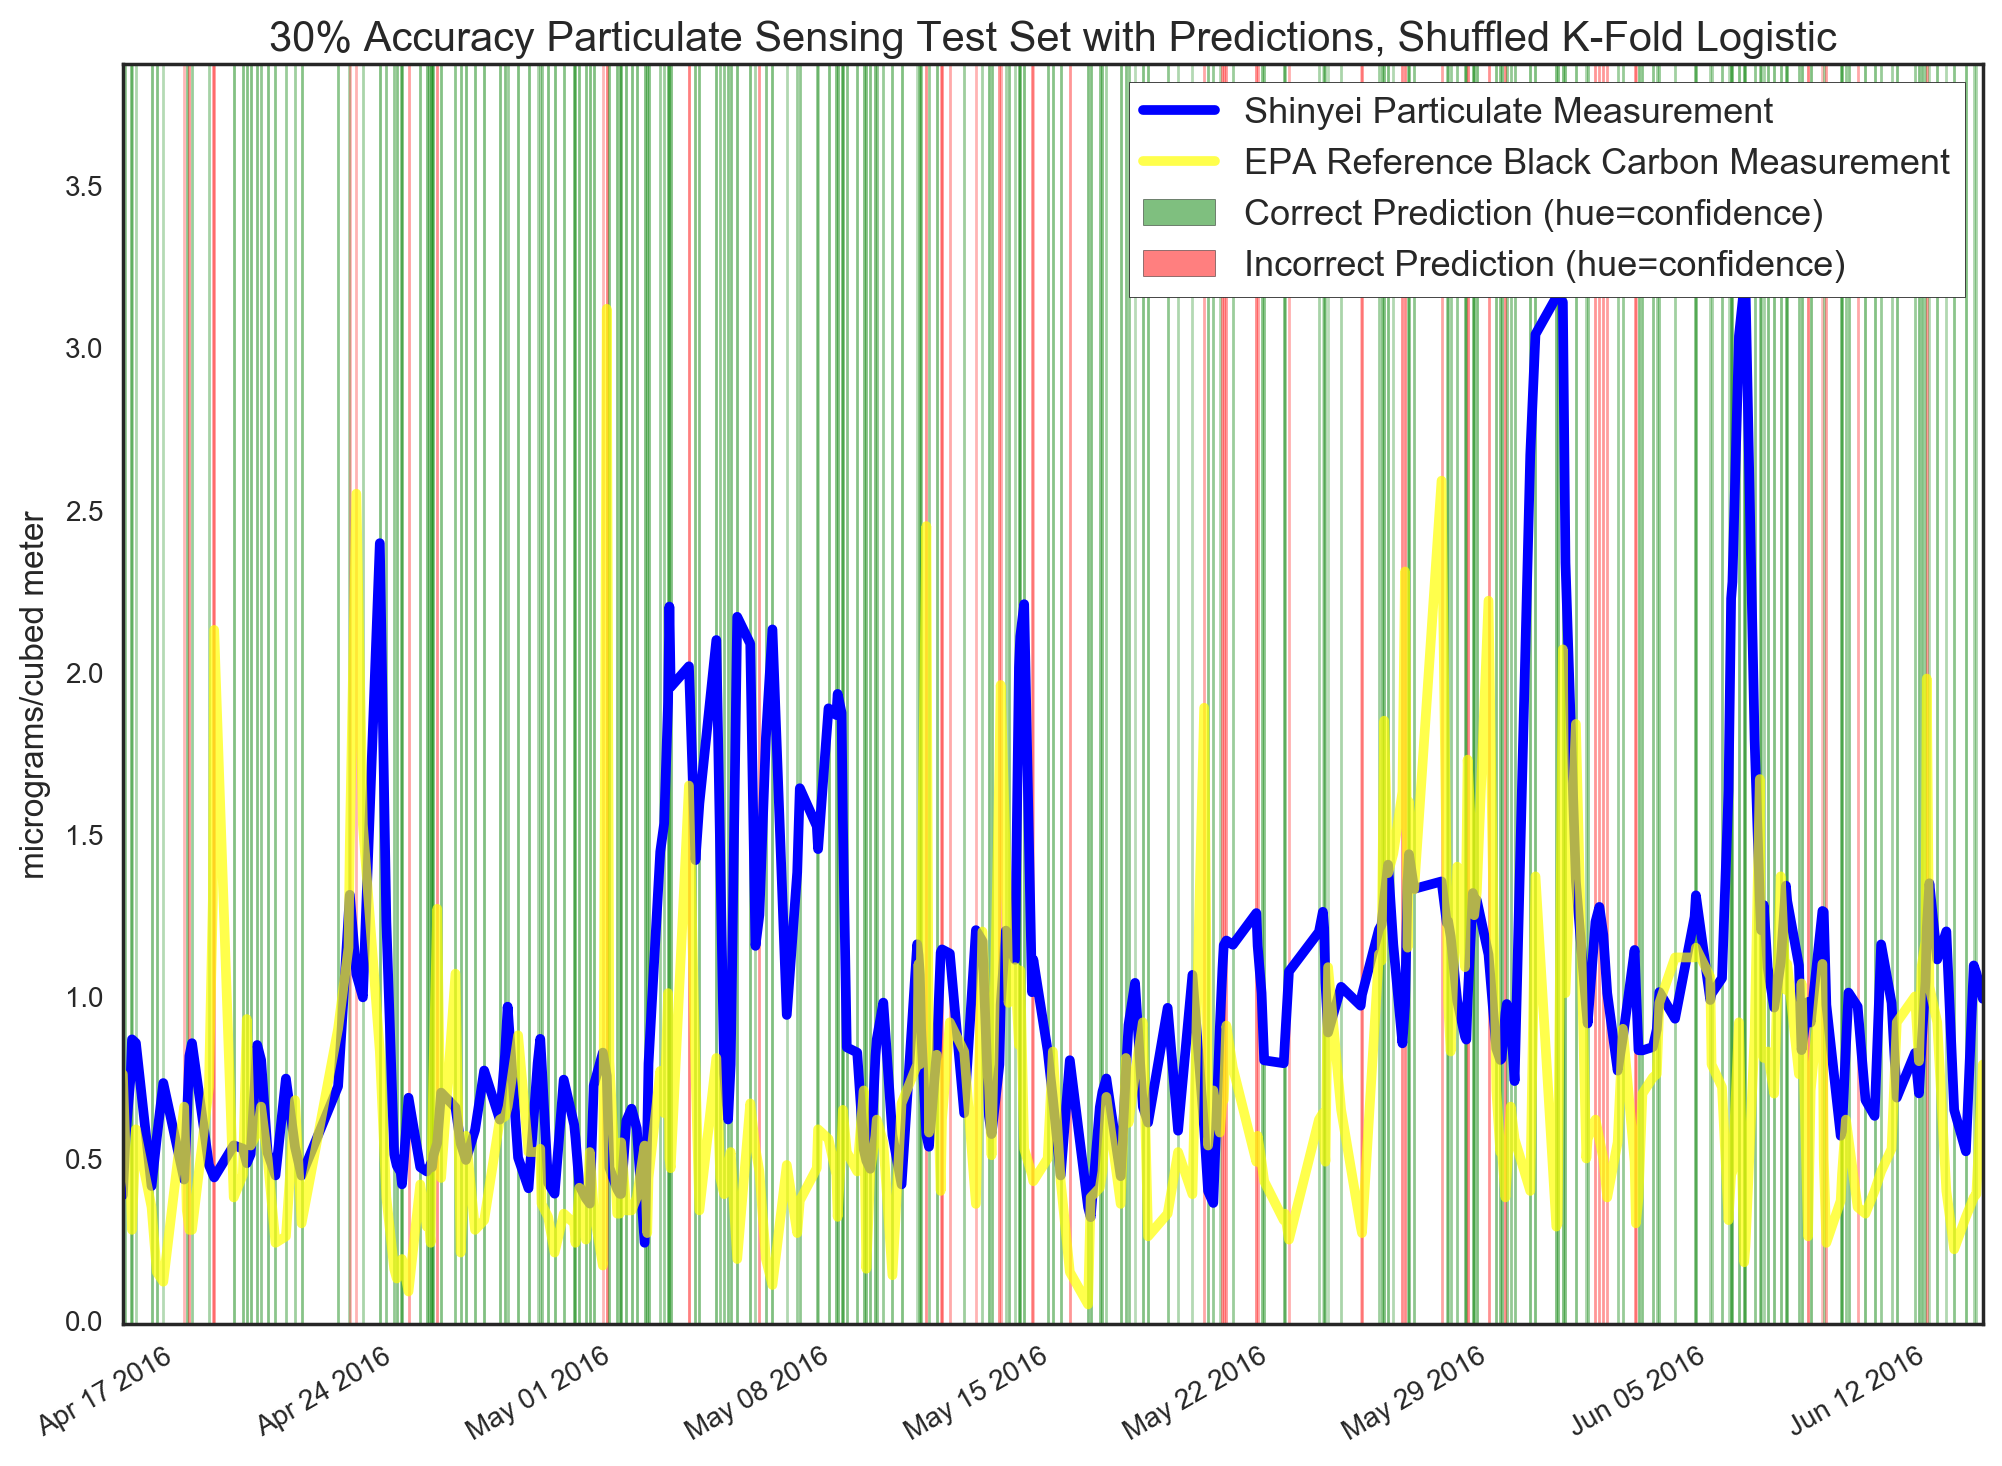
\includegraphics[width=\textwidth]{figs/sharp_goals_30_logistic_predictions}               
 	 \caption{Sharp Particulate Prediction Accuracy}
  	\label{fig:sharp_30_logistic_predictions}
\end{figure}

here's text referencing the (Table \ref{tab:sharp_randomforest_features}).

\begin{table}[H]
\centering
\begin{tabular}{lllllllll}
\\
\\
\toprule
Feature & Importance \\
\midrule
 scaled\_sharpDust &  0.039935725943 \\
 avg\_12\_scaled\_sharpDust &  0.0390147943972 \\
 sharpDust &  0.0390147211728 \\
 lmse\_scaled\_sharpDust &  0.0381632767126 \\
 avg\_48\_scaled\_sharpDust &  0.0225005941711 \\
 lmse\_avg\_48\_scaled\_sharpDust &  0.0207695248823 \\
 sck\_humidity &  0.0163292725576 \\
 Humidity ( \% RAW) &  0.0162400825573 \\
 no2 &  0.0149758603207 \\
 daily\_avg\_sck\_humidity &  0.0138699992039 \\
 daily\_avg\_forecastio\_humidity &  0.0132135840929 \\
 humidity\_box\_differential &  0.0119641893085 \\
 co &  0.0118968560369 \\
 sck\_humidity\_saturated &  0.0103888721788 \\
 avg\_60\_forecastio\_humidity &  0.0102980544091 \\
\bottomrule
\end{tabular}
\label{tab:sharp_randomforest_features}
\caption{Top 15 Features from Random Forest for Sharp Sensor, used in Pruned Logistic Regression}
\end{table}


\begin{figure}[htb]
 	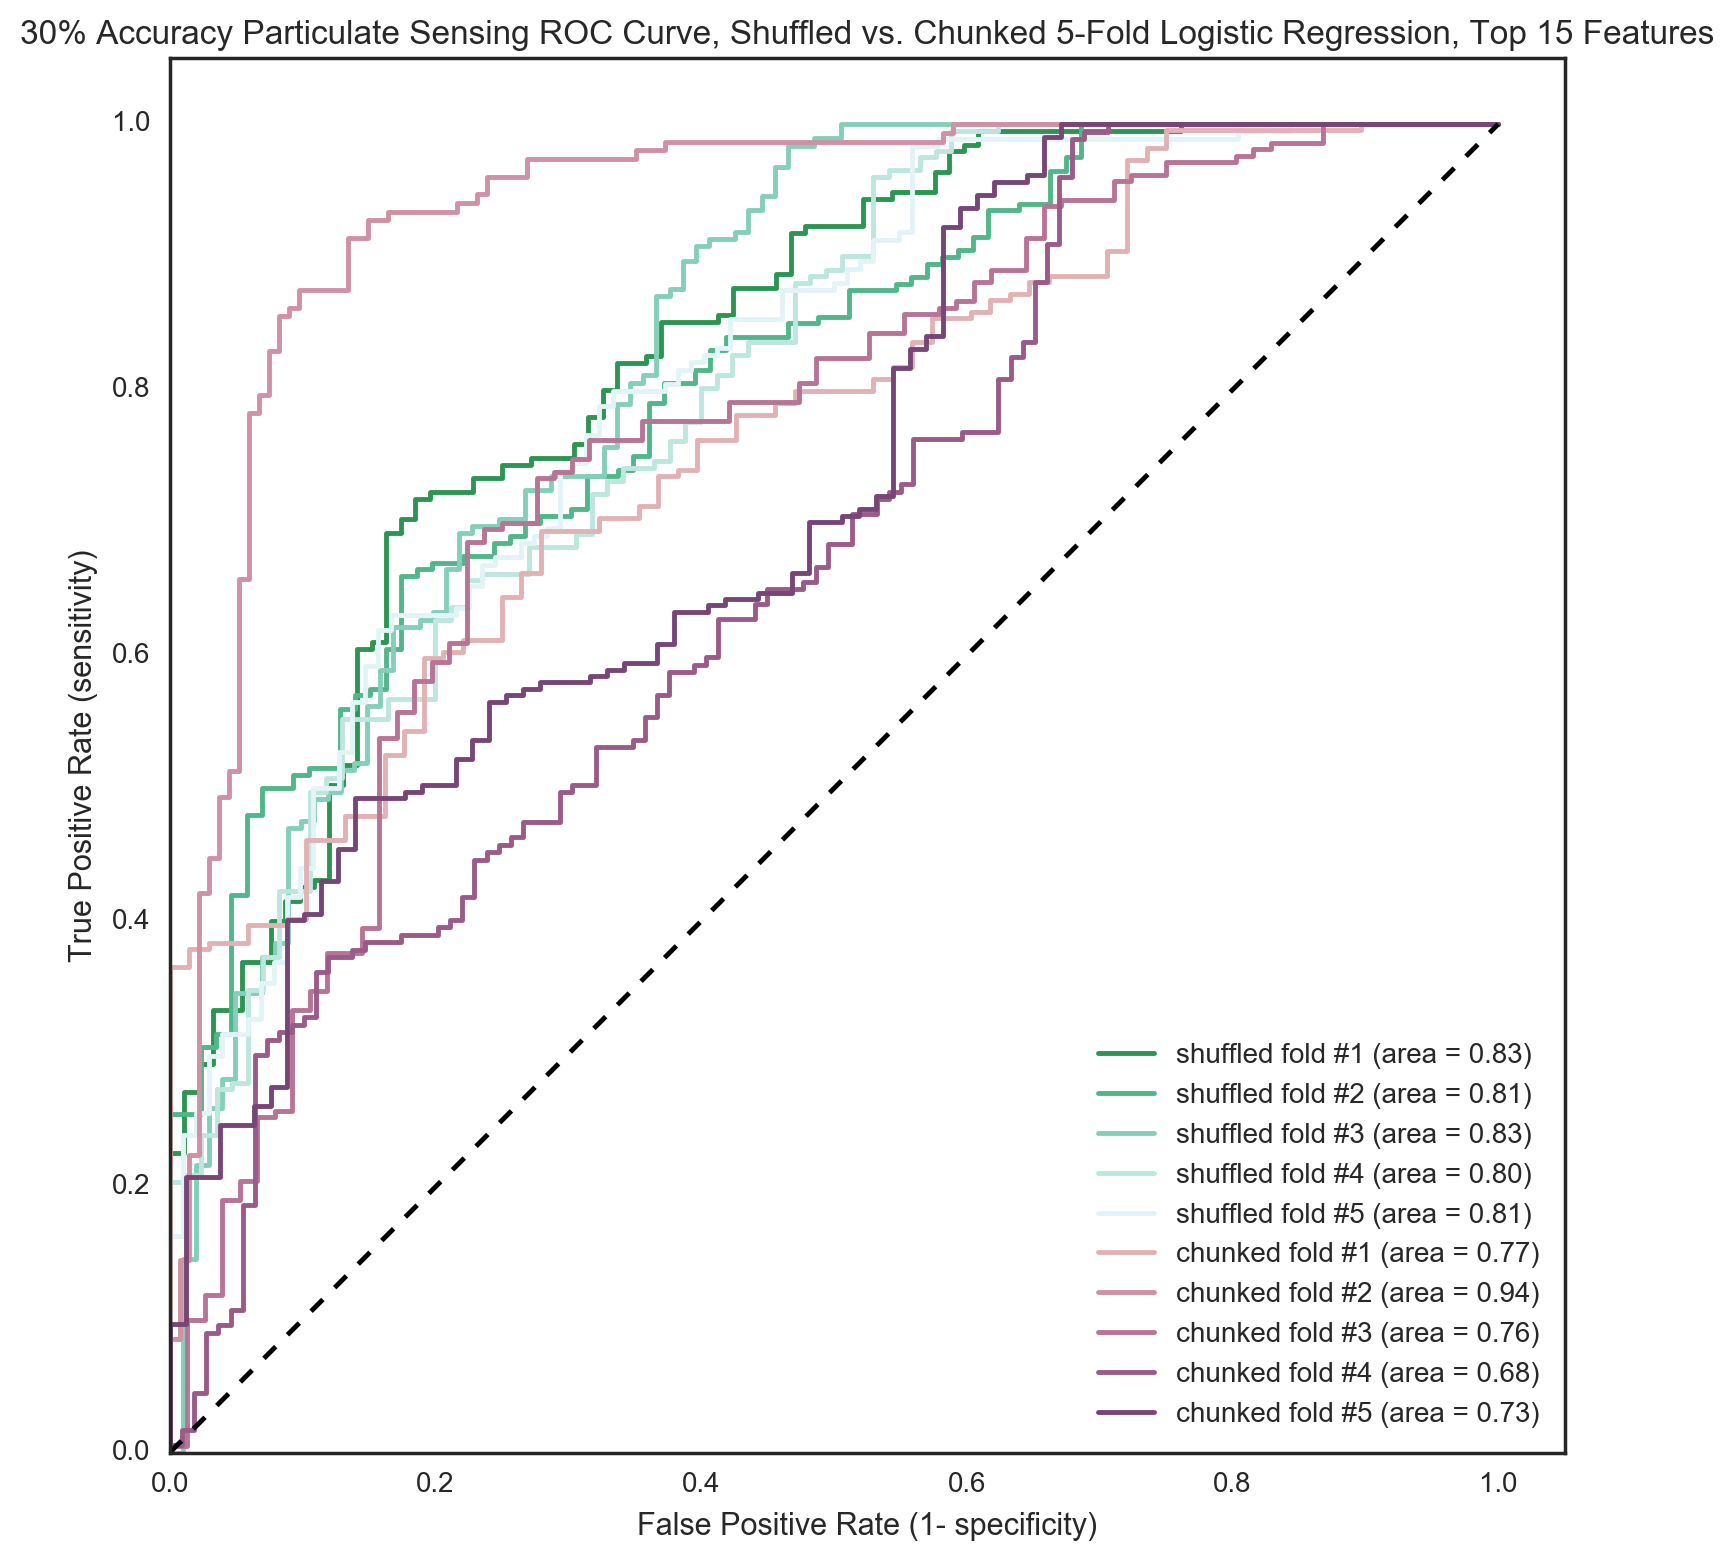
\includegraphics[width=\textwidth]{figs/sharp_goals_30_roc_pruned_features}               
 	 \caption{Sharp Particulate ROC Using Top 15 Features}
  	\label{fig:sharp_30_roc_pruned_features}
\end{figure}


\begin{figure}[htb]
 	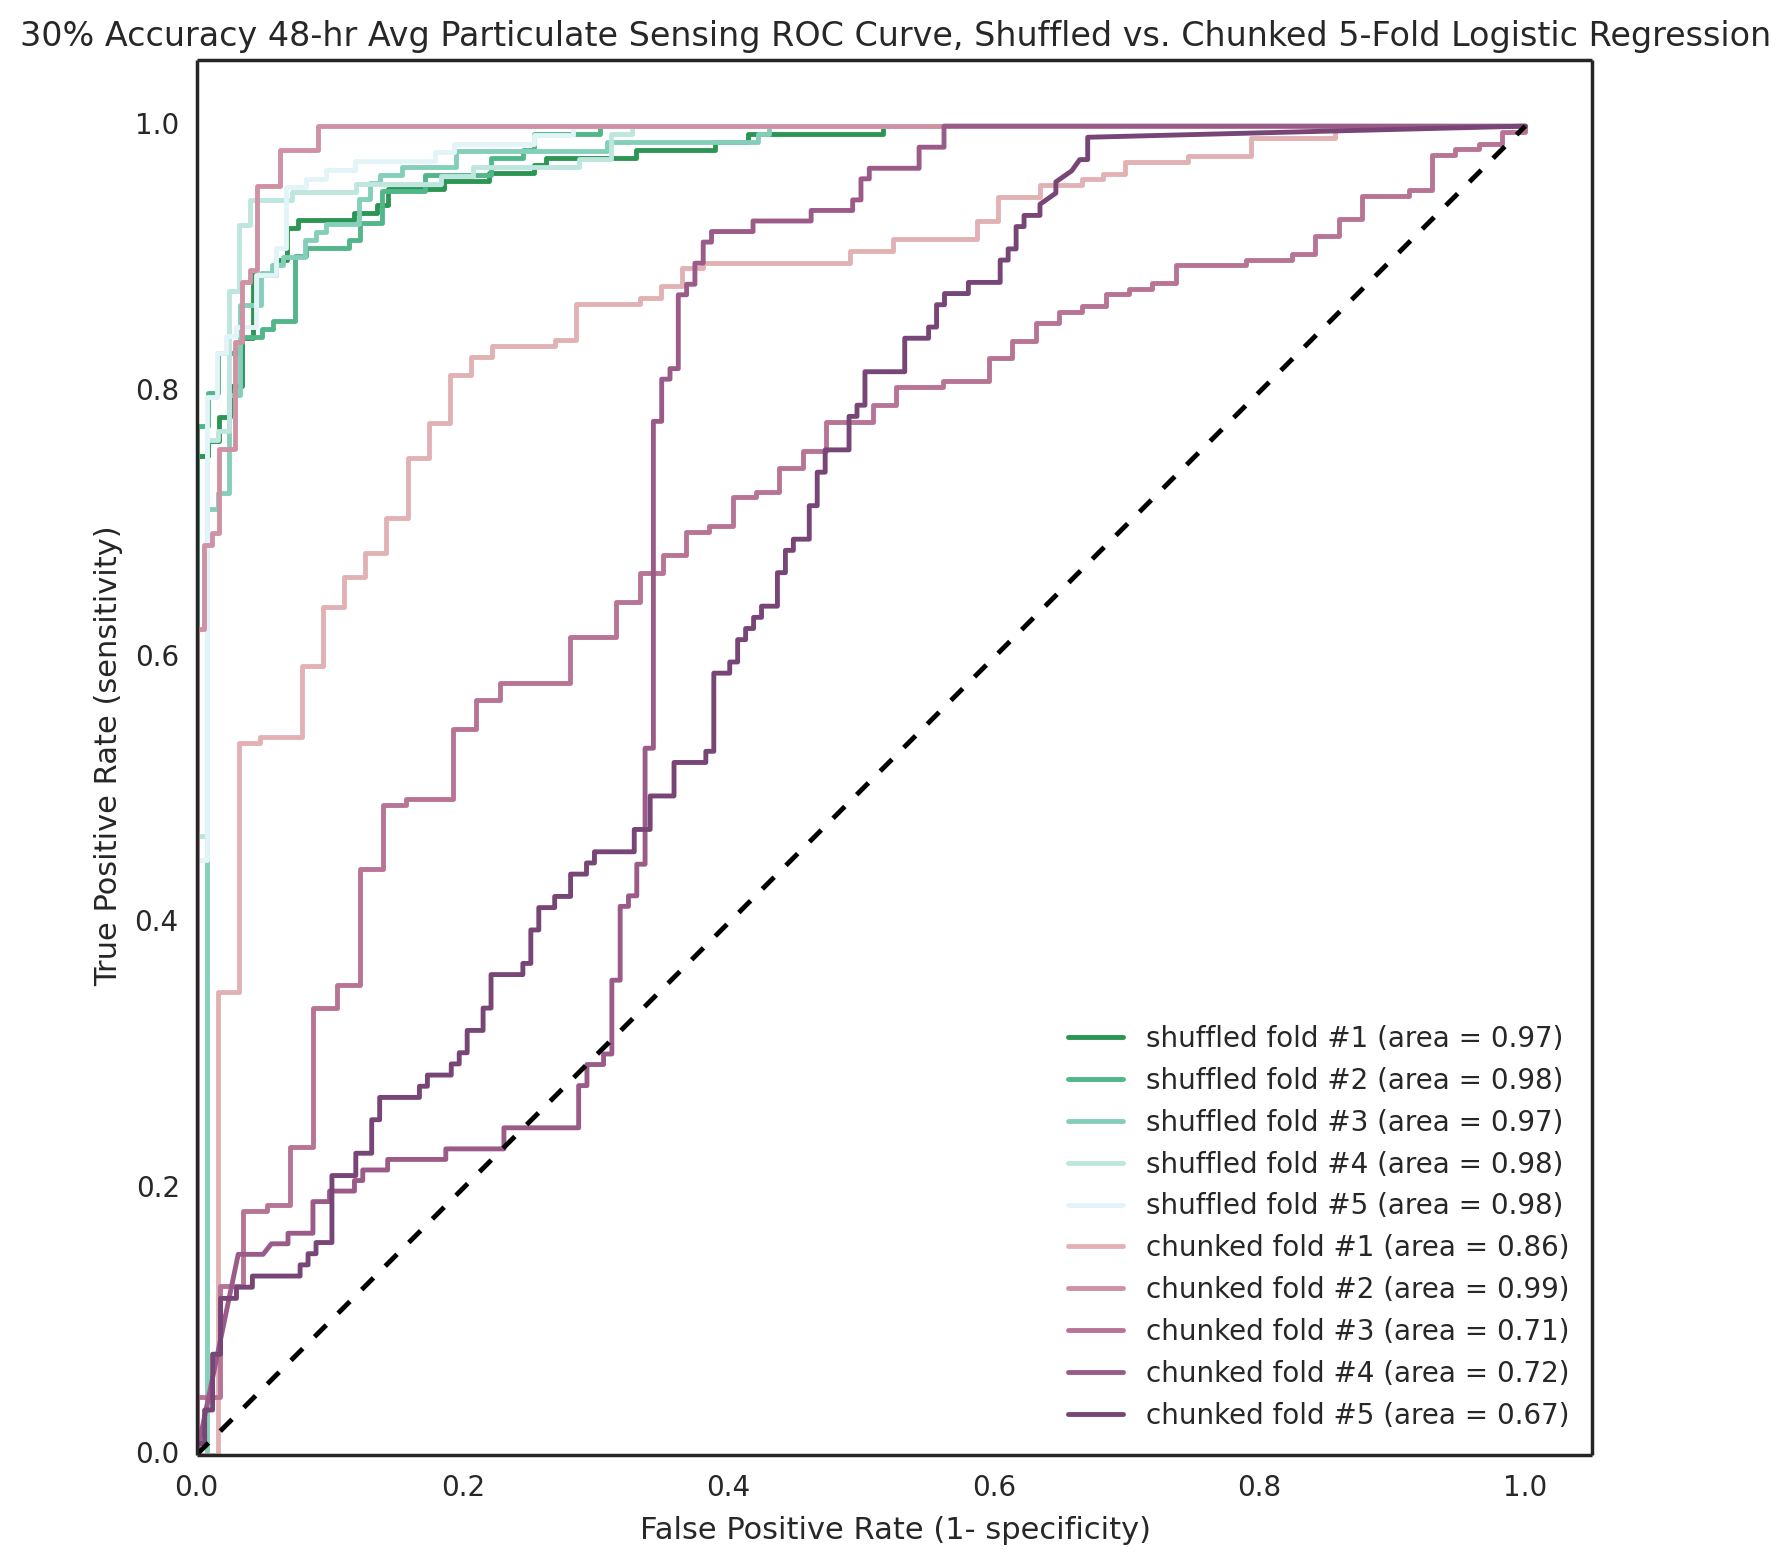
\includegraphics[width=\textwidth]{figs/sharp_48_avg_goals_30_roc}               
 	 \caption{48-hour Average Sharp Particulate ROC}
  	\label{fig:sharp_48_avg_goals_30_roc}
\end{figure}

\begin{figure}[htb]
 	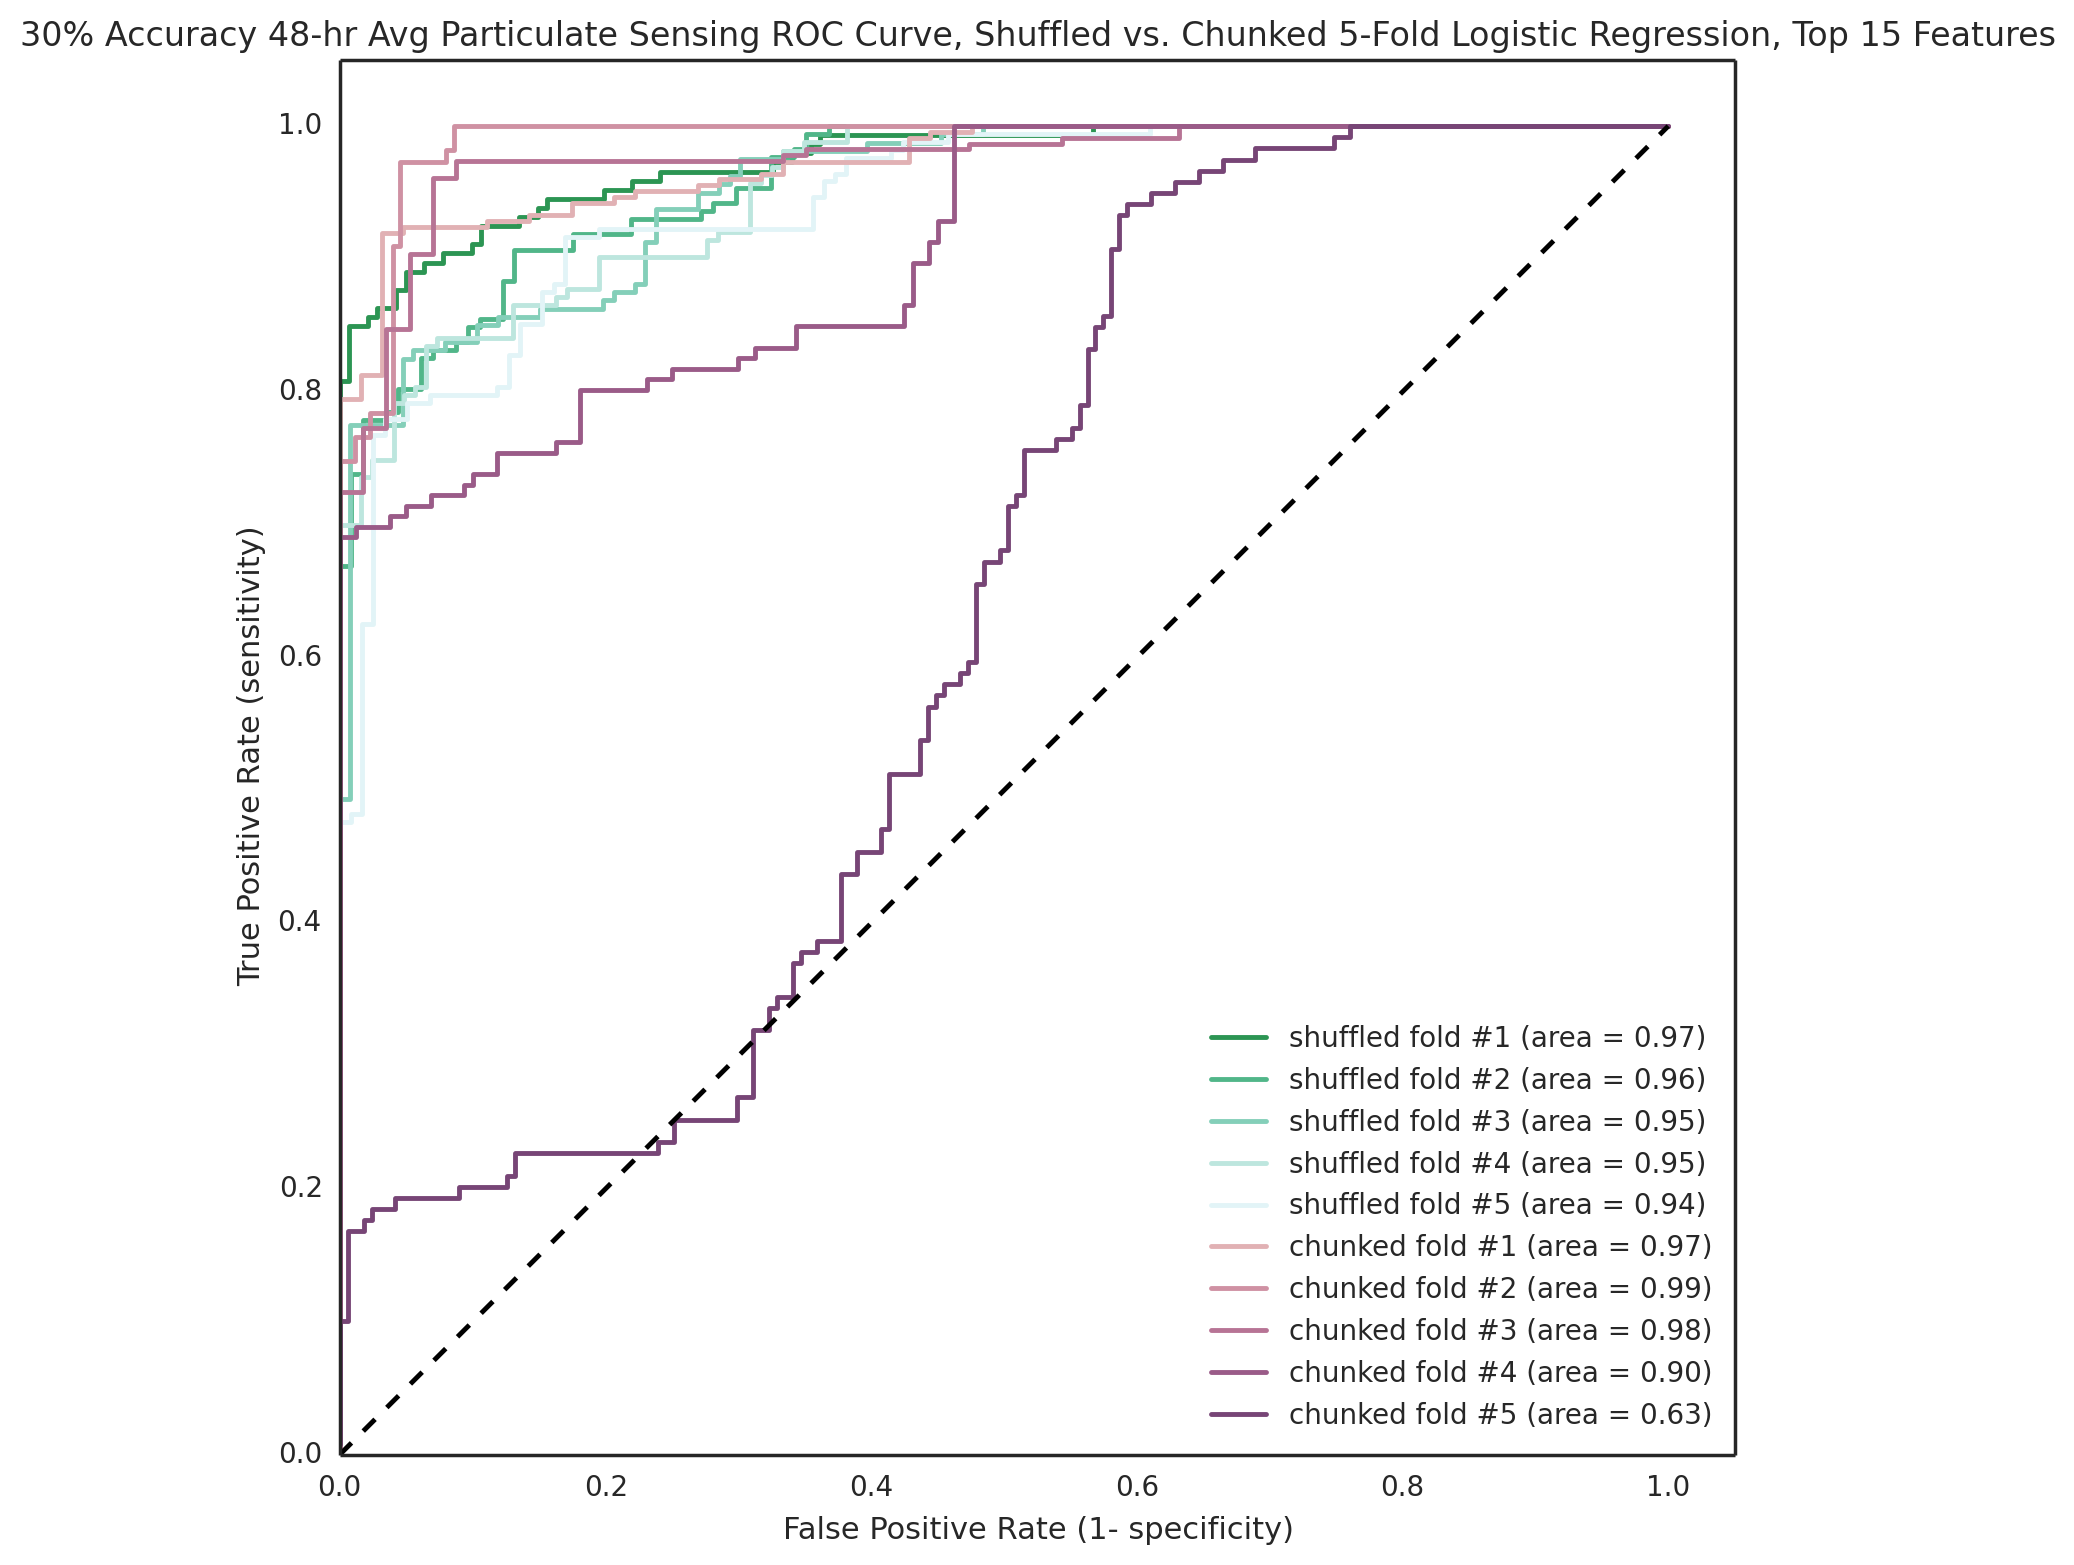
\includegraphics[width=\textwidth]{figs/sharp_48_avg_goals_30_roc_pruned_features}               
 	 \caption{48-hour Average Sharp Particulate ROC Using Top 15 Features}
  	\label{fig:sharp_48_avg_goals_30_roc_pruned_features}
\end{figure}

\begin{figure}[htb]
 	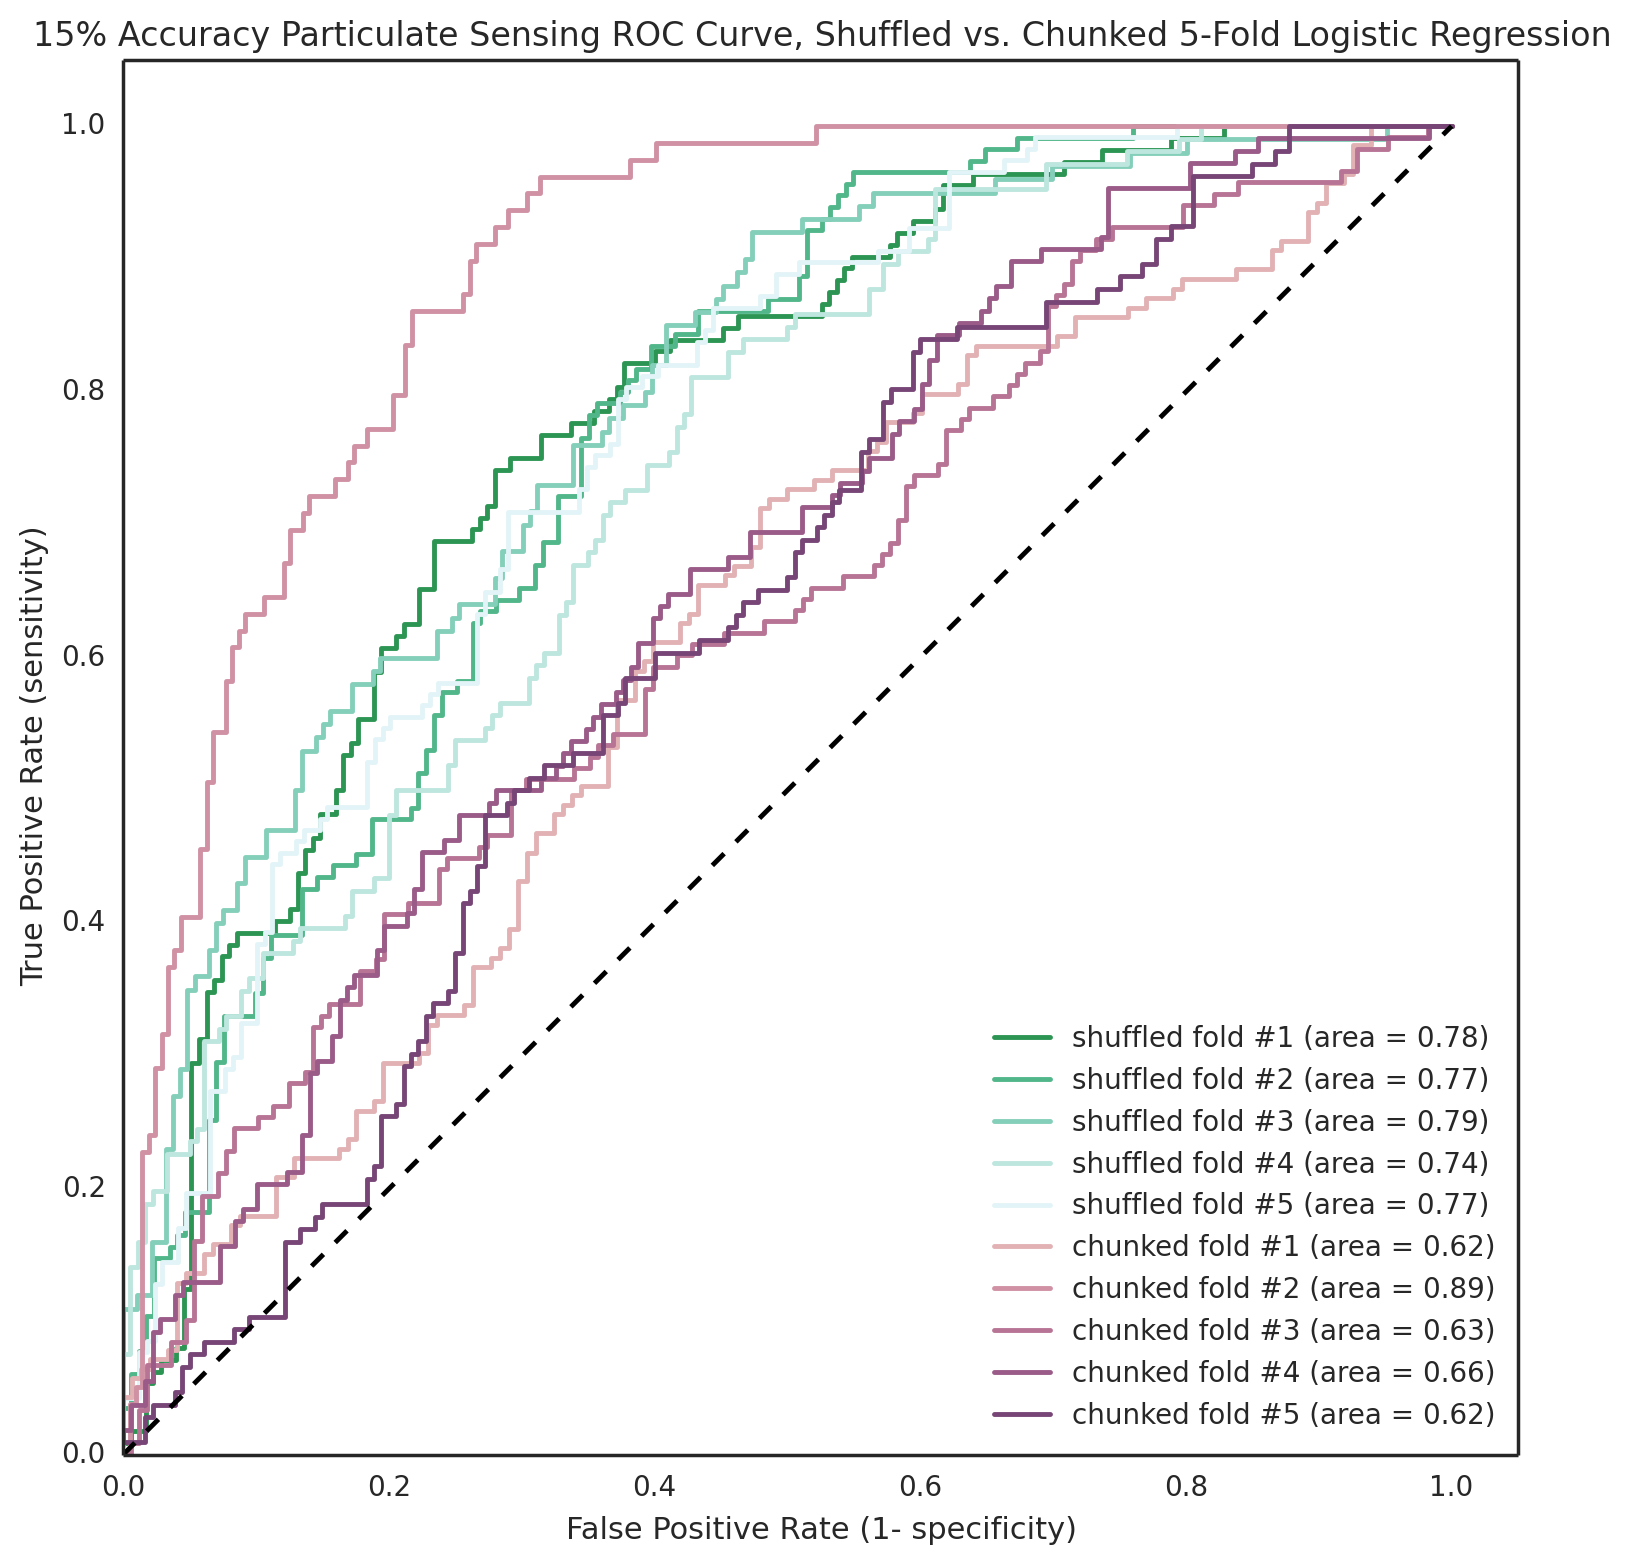
\includegraphics[width=\textwidth]{figs/sharp_goals_15_roc}               
 	 \caption{Reduced Tolerance Sharp Particulate ROC}
  	\label{fig:sharp_goals_15_roc}
\end{figure}

\begin{figure}[htb]
 	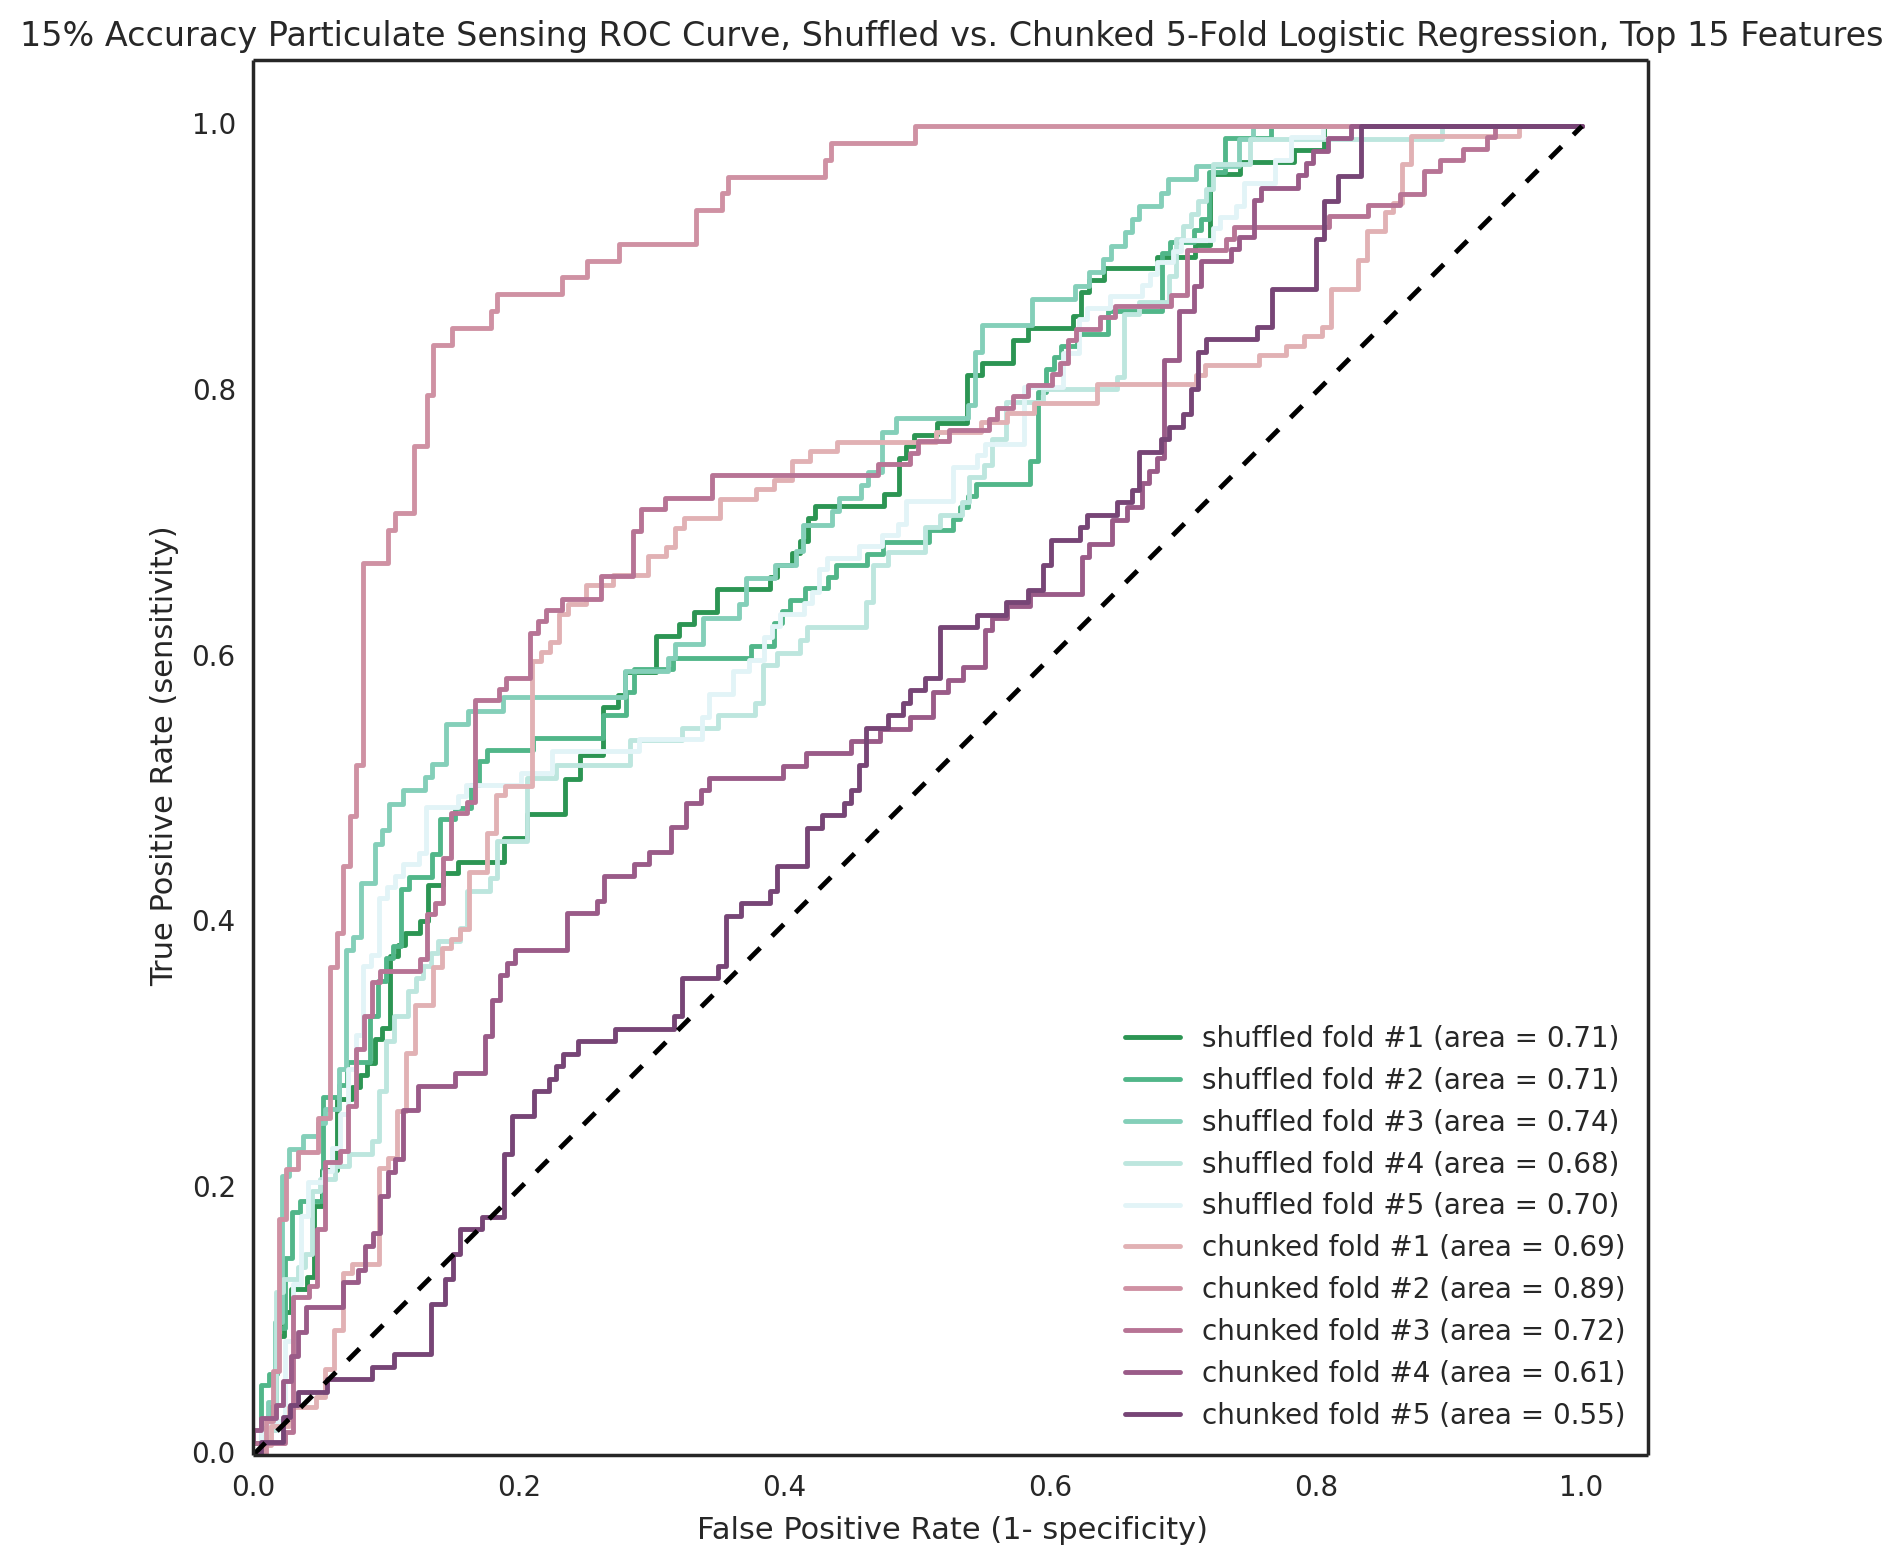
\includegraphics[width=\textwidth]{figs/sharp_goals_15_roc_pruned_features}               
 	 \caption{Reduced Tolerance Sharp Particulate ROC Using Top 15 Features}
  	\label{fig:sharp_goals_15_roc_pruned_features}
\end{figure}

\FloatBarrier
\section{AlphaSense CO}
\FloatBarrier

\begin{figure}[htb]
 	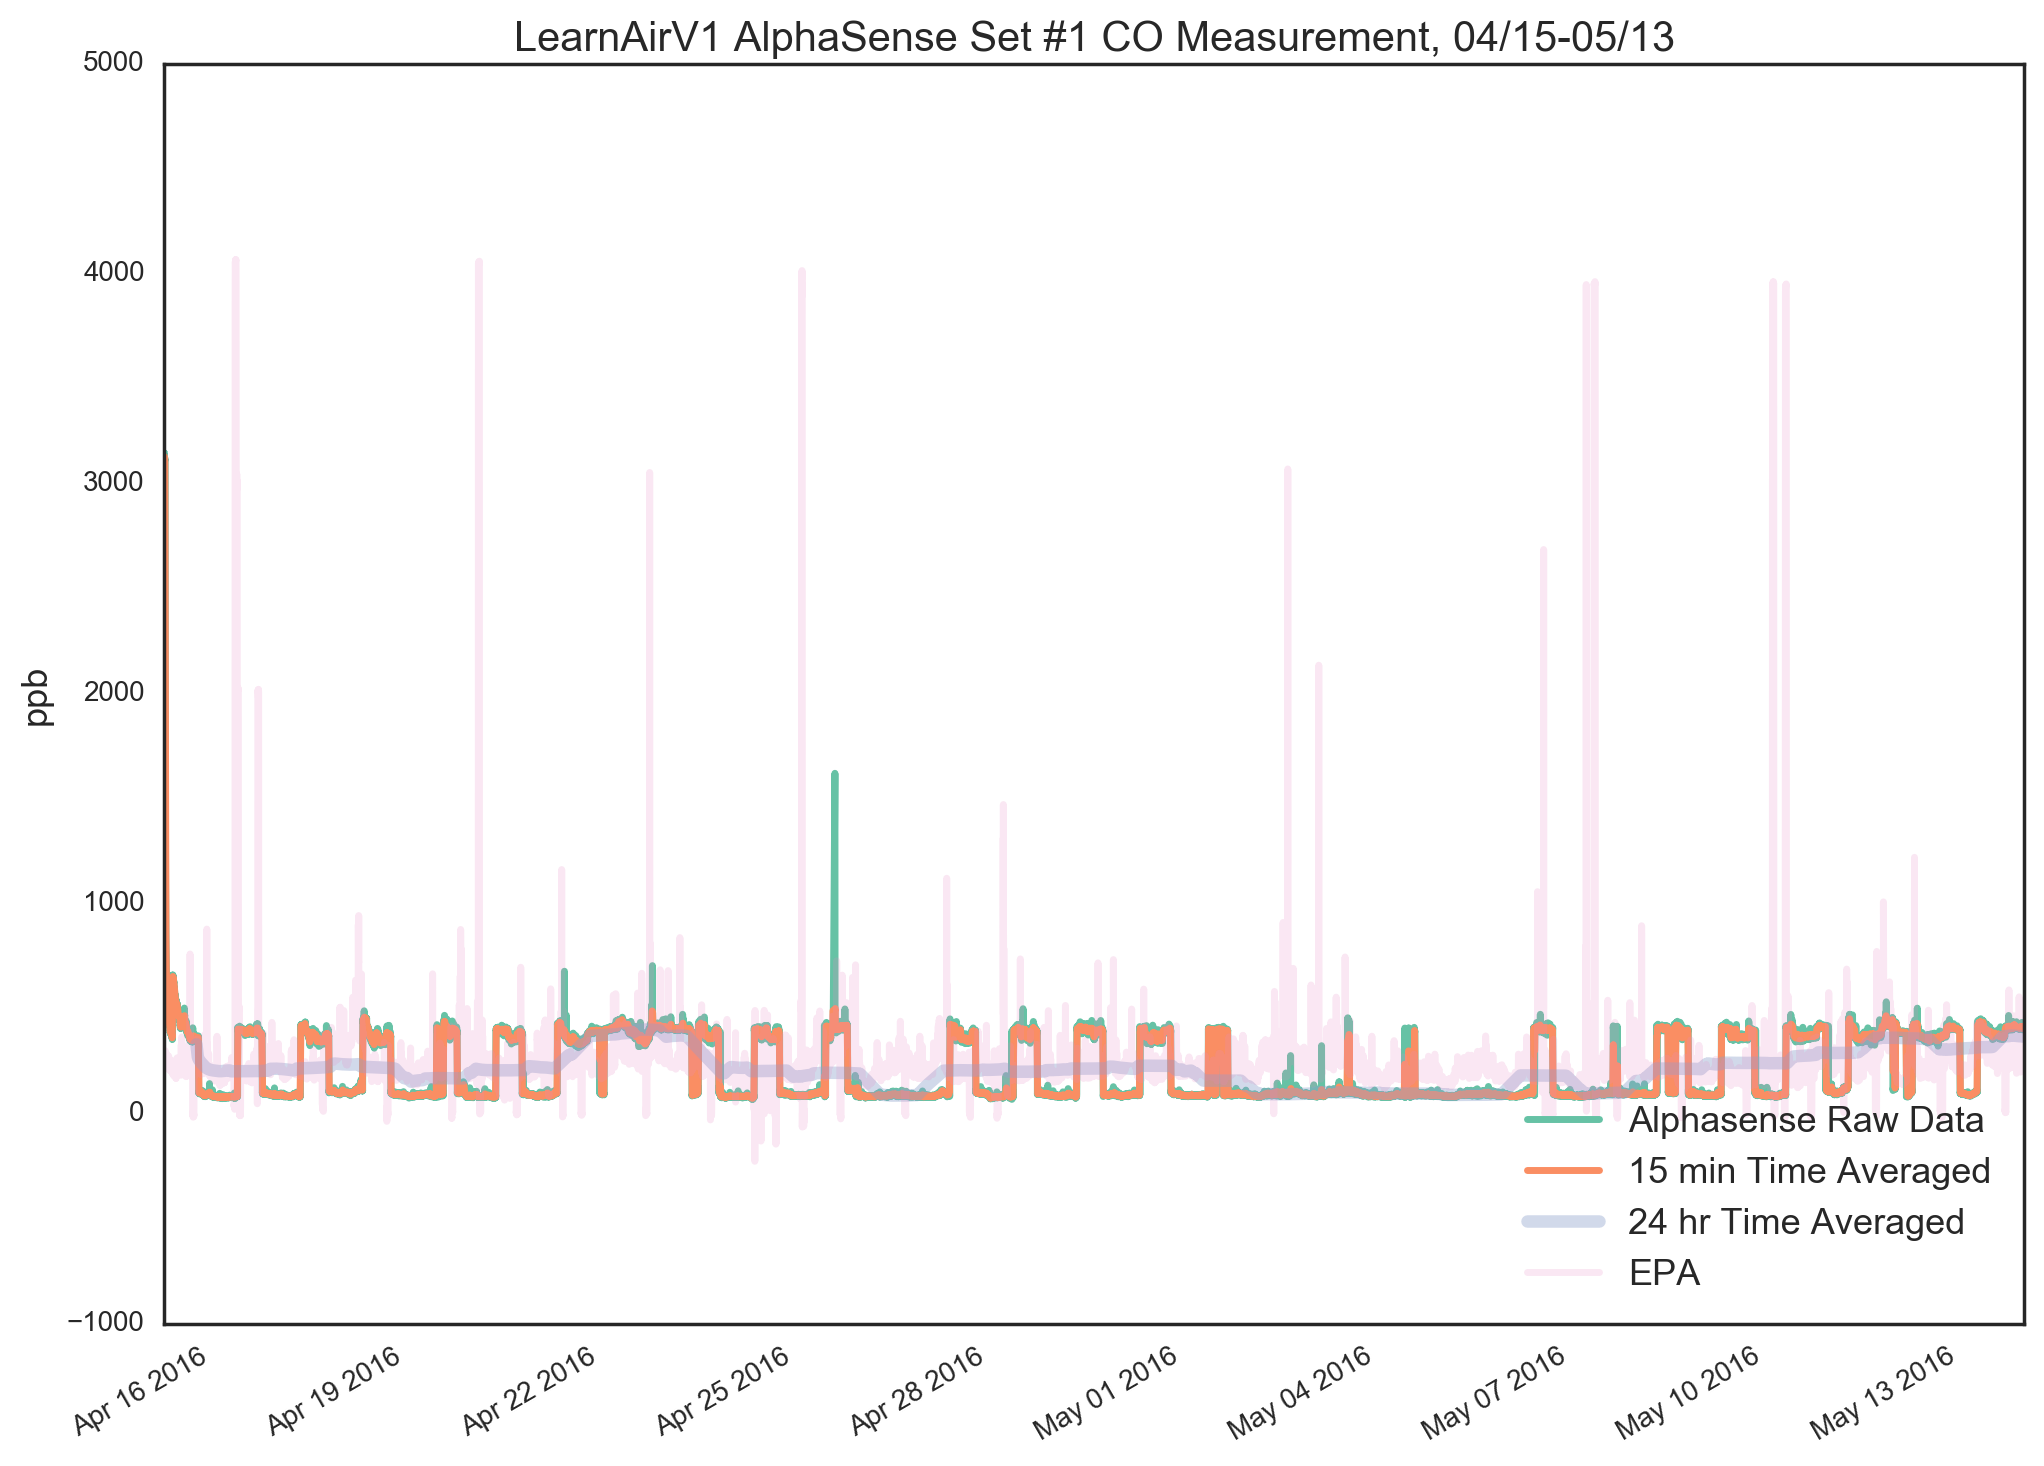
\includegraphics[width=\textwidth]{figs/as_co_raw}               
 	 \caption{AlphaSense CO Sensor #1 Raw Data}
  	\label{fig:as_co_raw}
\end{figure}

\begin{figure}[htb]
 	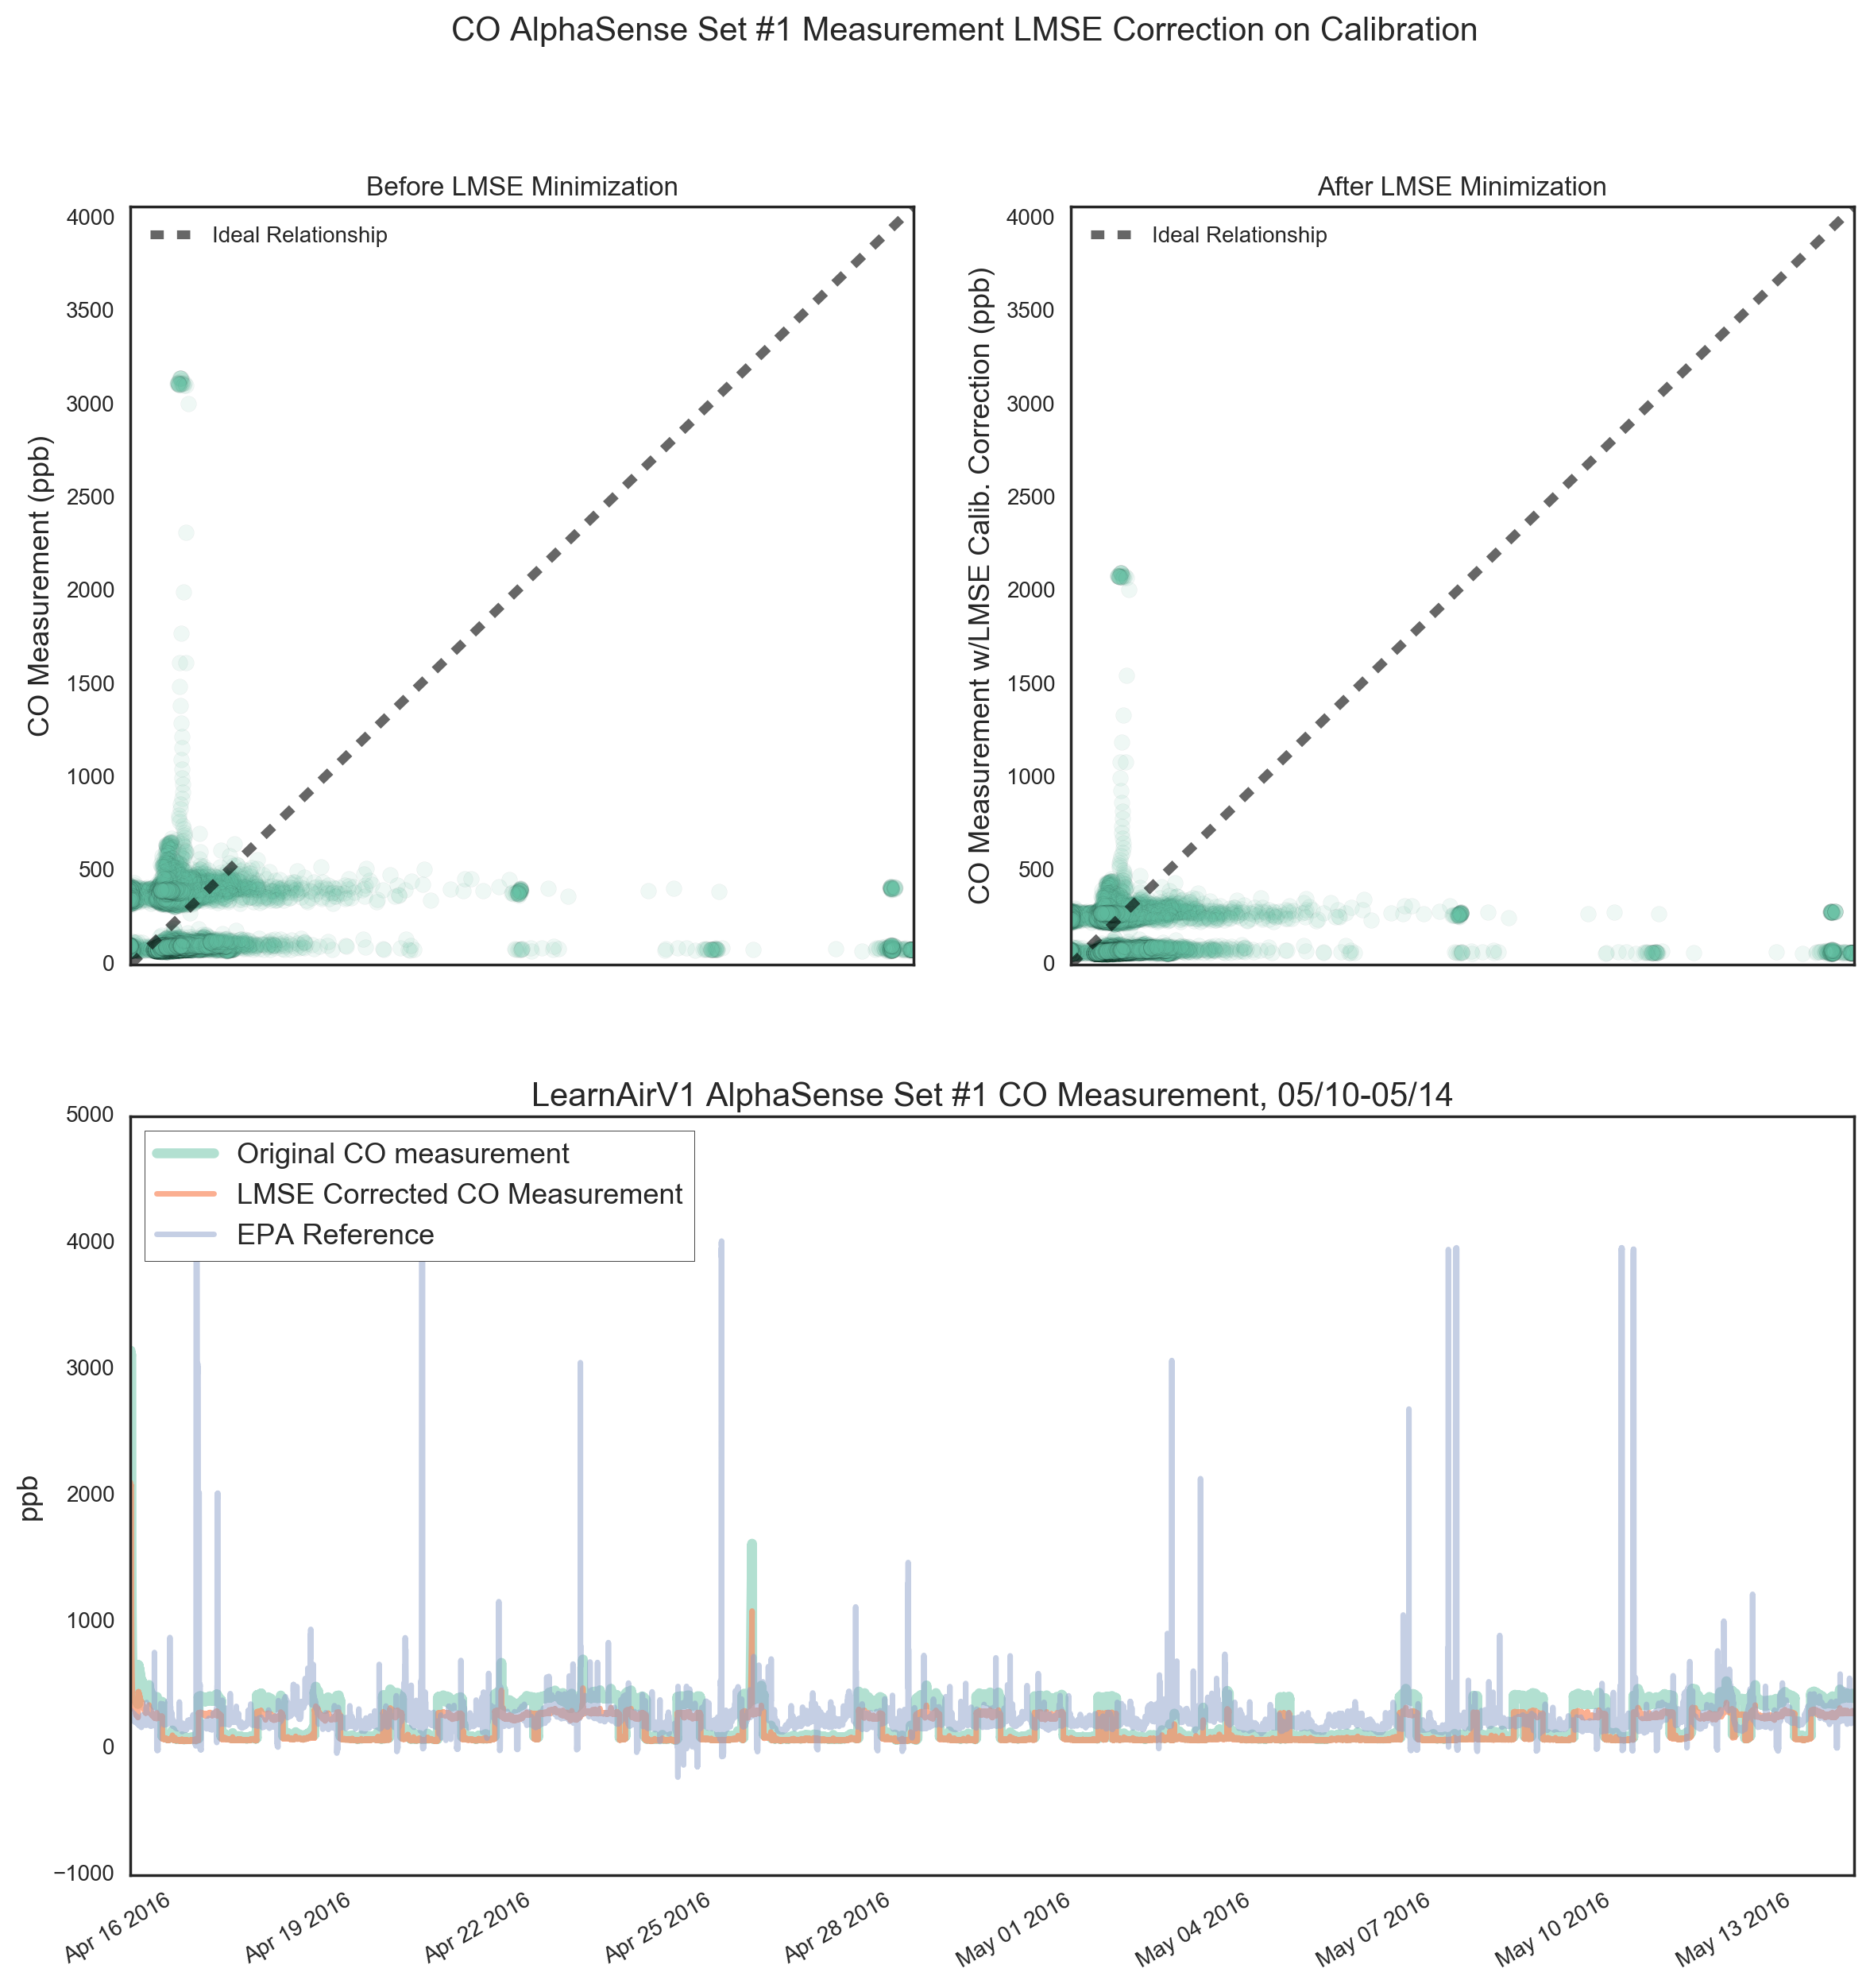
\includegraphics[width=\textwidth]{figs/as1_co_lmse}               
 	 \caption{AlphaSense CO Sensor #1 after LMSE Calibration}
  	\label{fig:as1_co_lmse}
\end{figure}

\begin{figure}[htb]
 	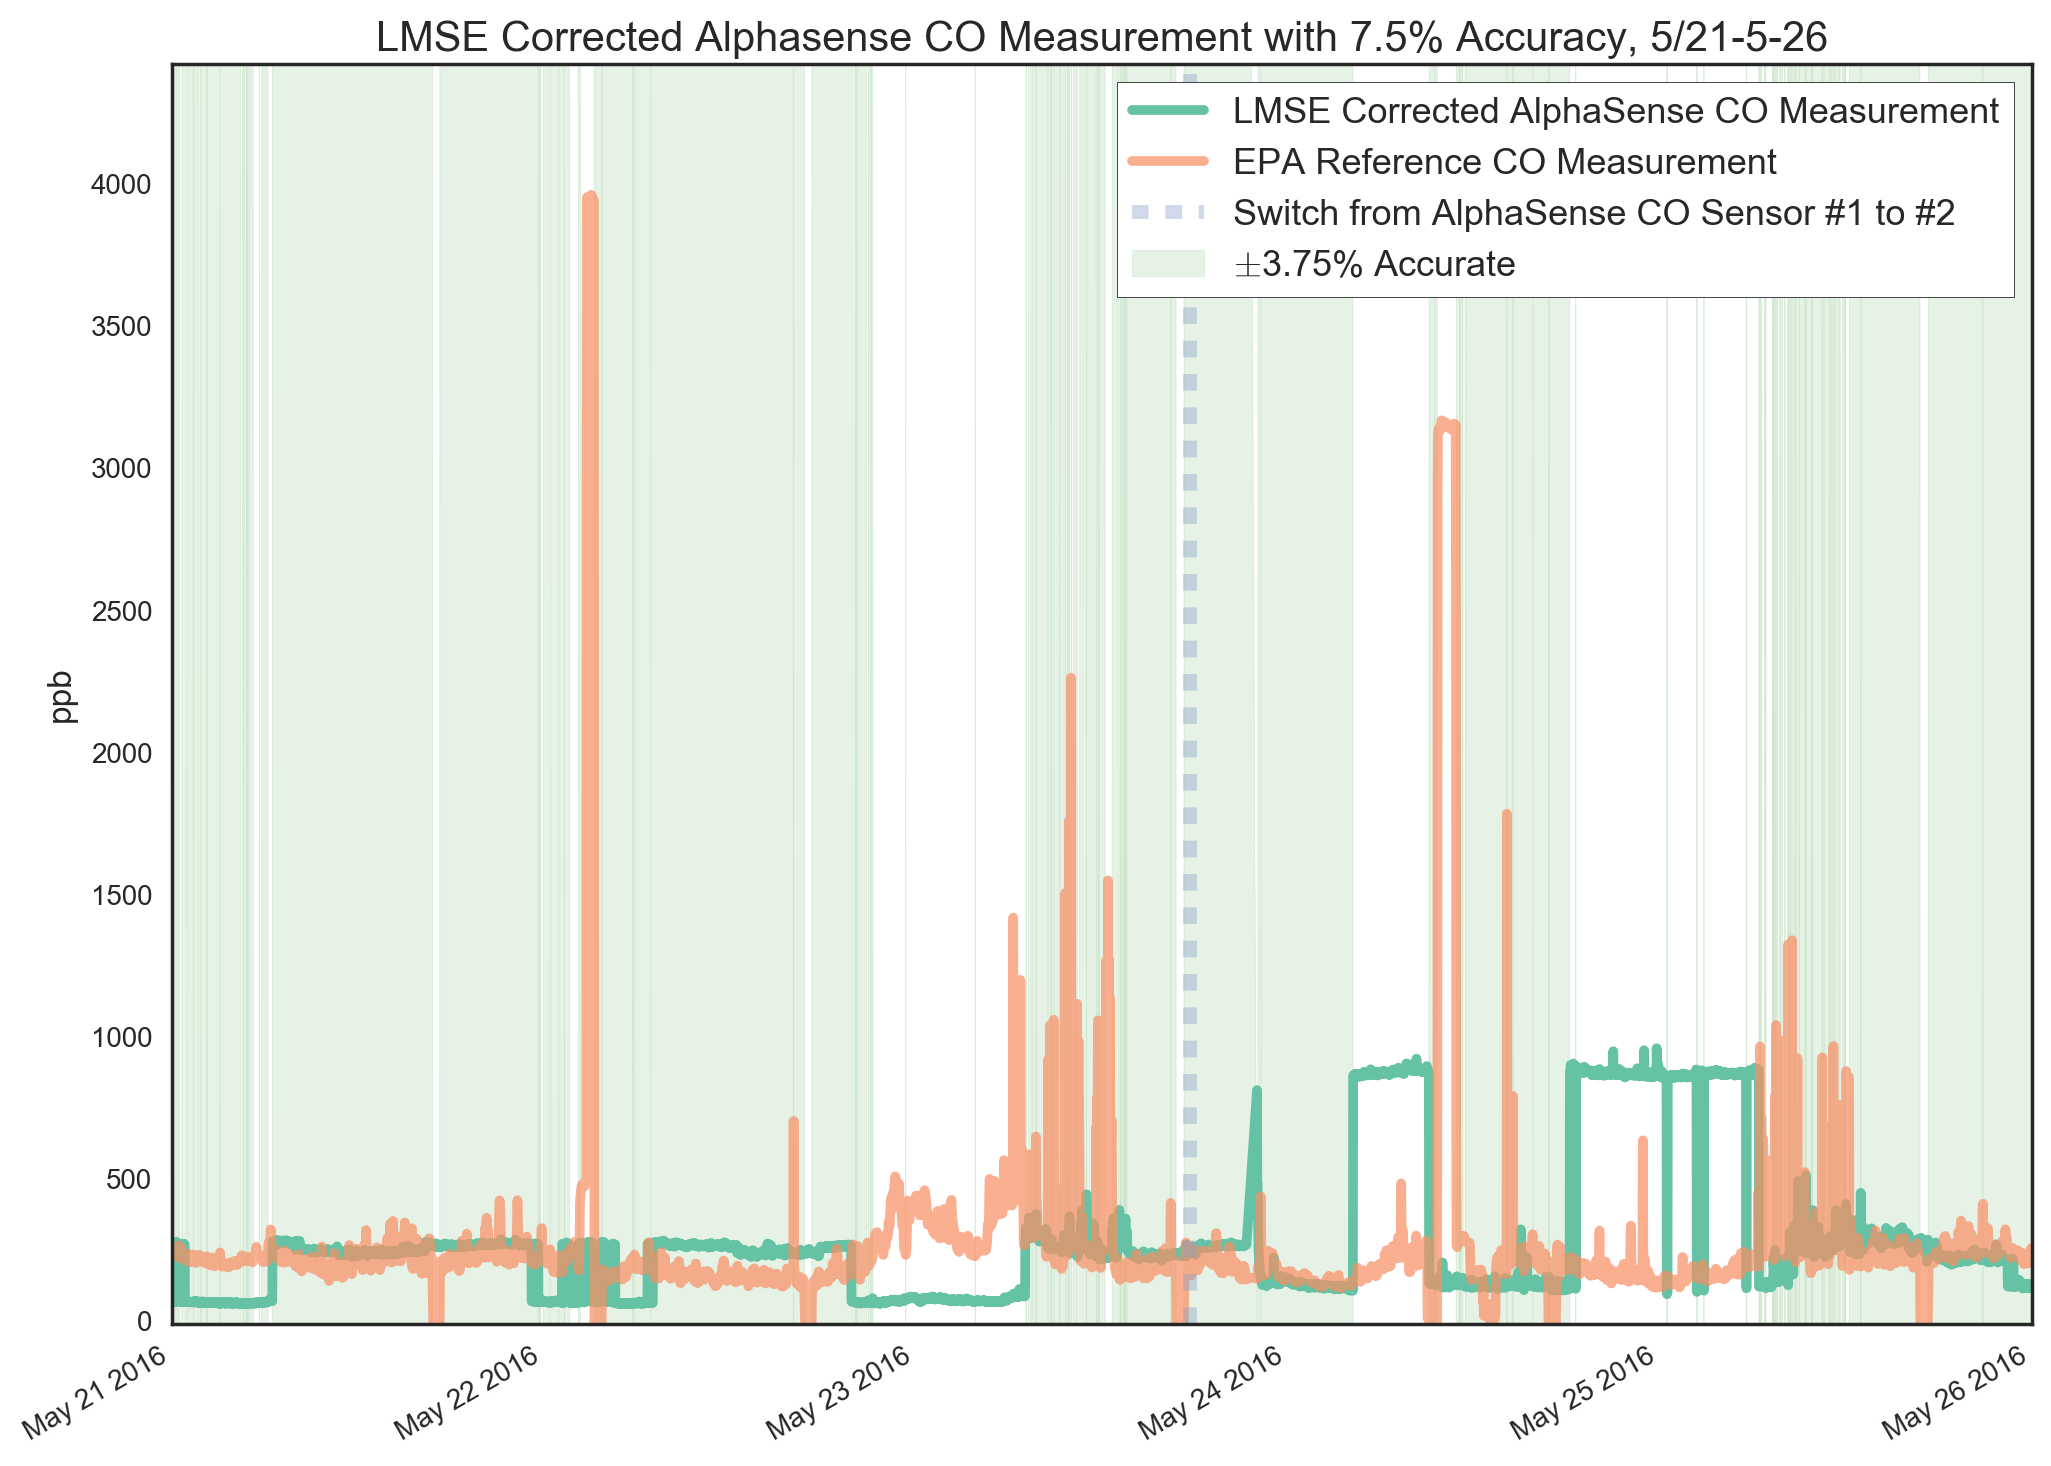
\includegraphics[width=\textwidth]{figs/as_co_with_7p5_accuracy_zoomed}               
 	 \caption{AlphaSense CO Sensor #1 and #2 with 7.5\% Accuracy Threshold}
  	\label{fig:as_co_with_7p5_accuracy_zoomed}
\end{figure}

\begin{figure}[htb]
 	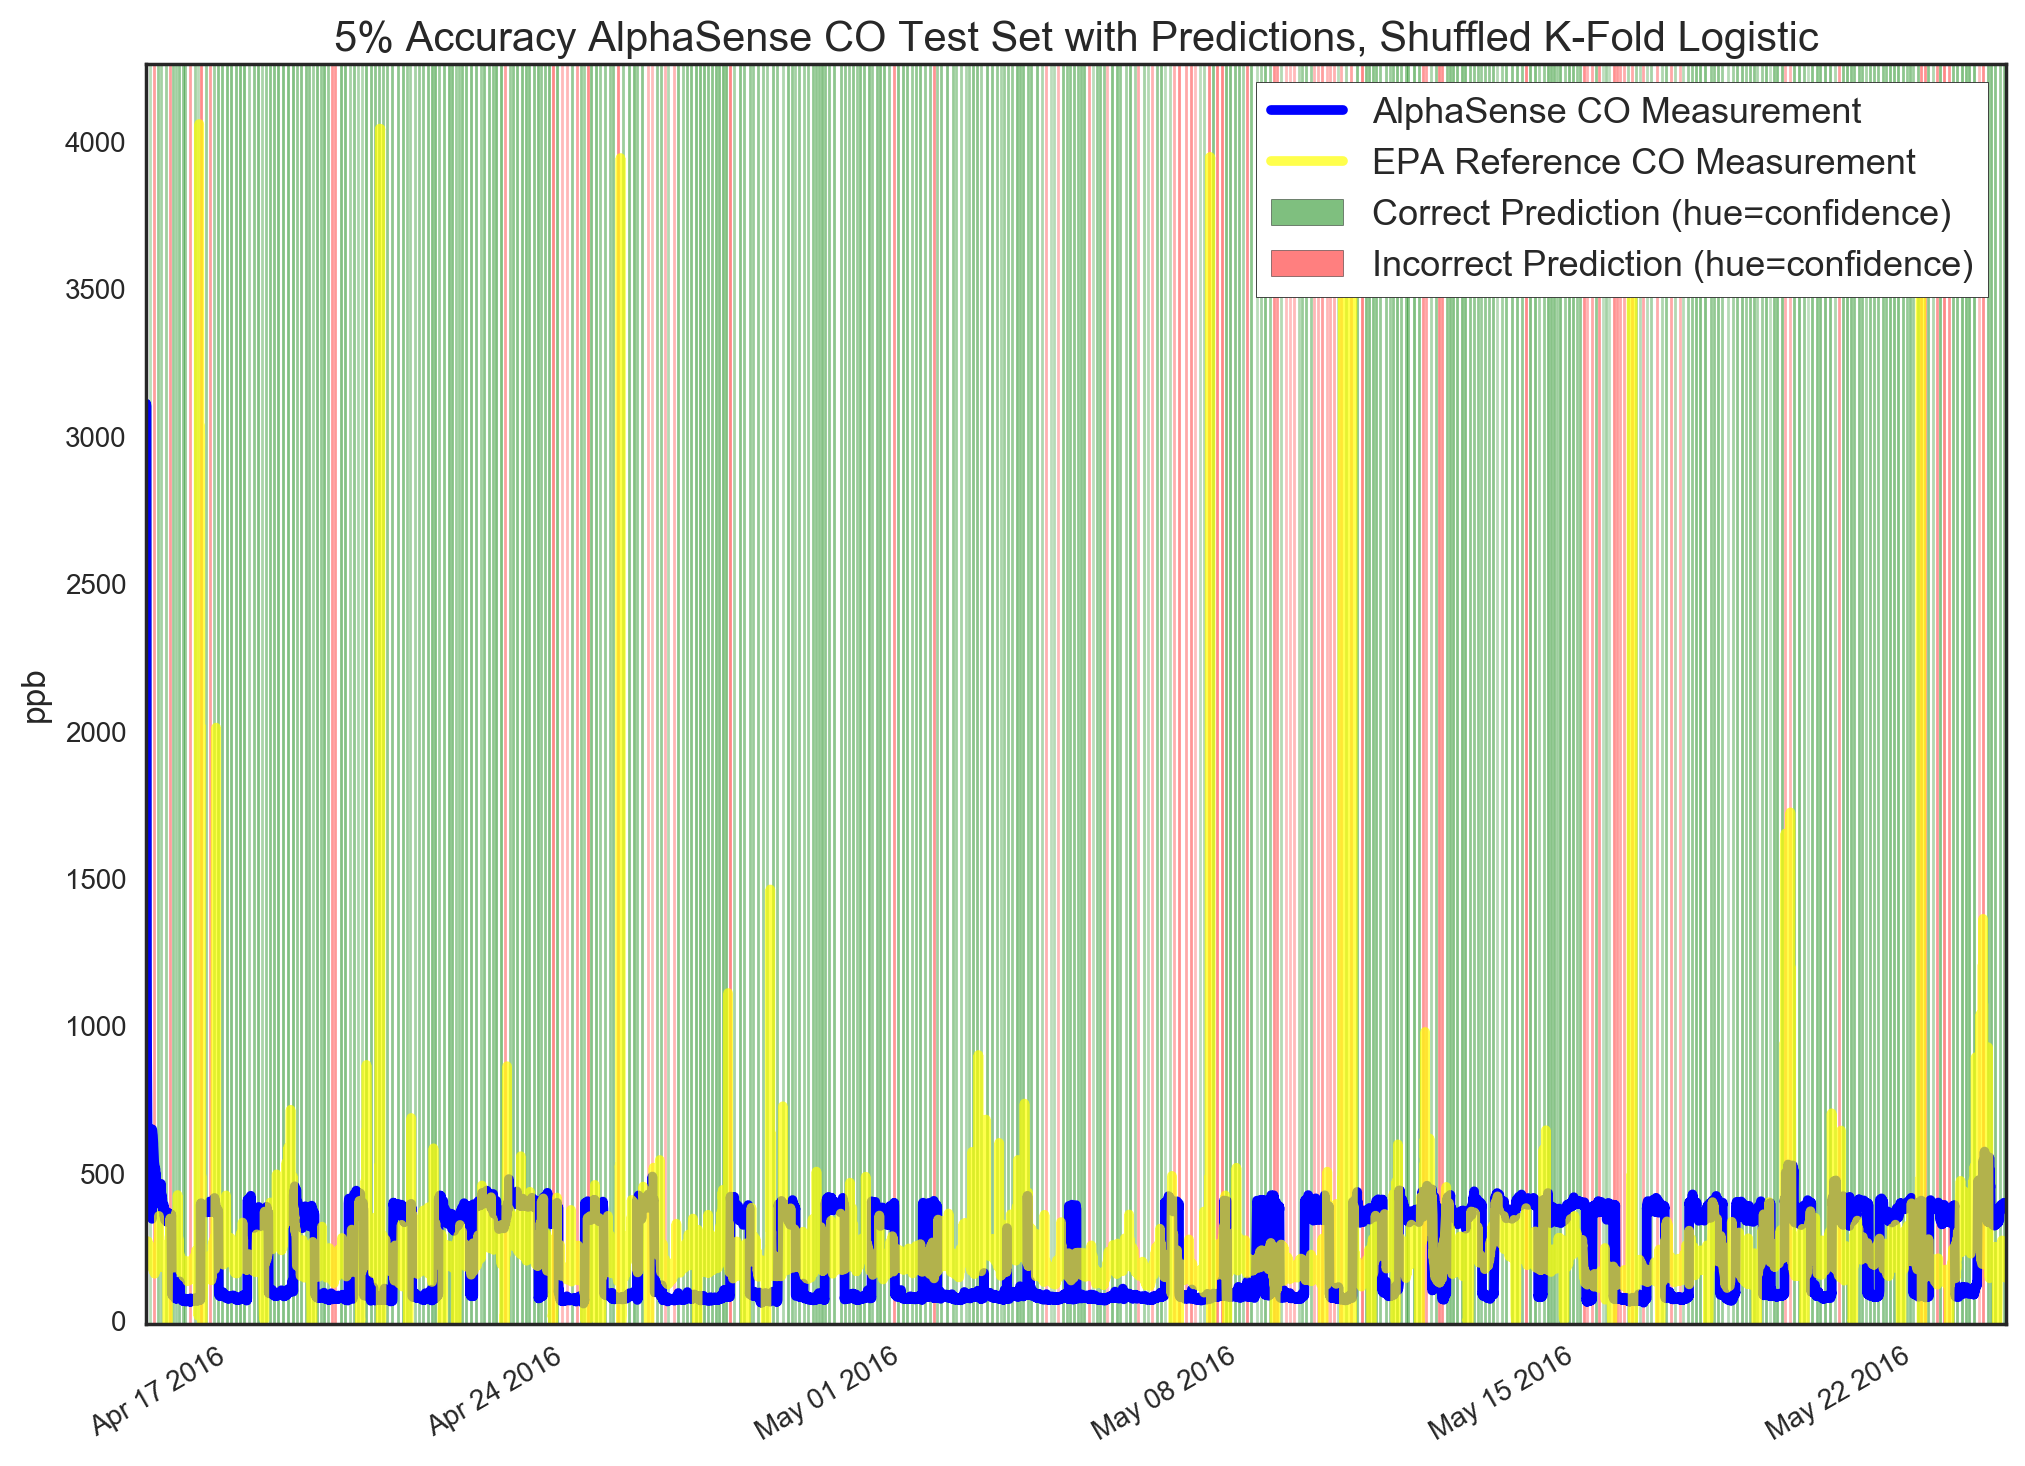
\includegraphics[width=\textwidth]{figs/as1_co_5_logistic_predictions}               
 	 \caption{AlphaSense CO Sensor #1 Prediction Accuracy}
  	\label{fig:as1_co_5_logistic_predictions}
\end{figure}

here's text referencing the (Table \ref{tab:as1_co_randomforest_features}).

\begin{table}[]
\centering
\small
\begin{tabular}{lllllllll}
\\
\\
\toprule
Feature & Importance \\
\midrule
lmse\_calib\_as\_co & 0.0331983839664 \\
avg\_15\_lmse\_calib\_as\_co & 0.0331946346979 \\
avg\_15\_as\_co & 0.0322602817136 \\
as\_co & 0.0310204625161 \\
sck\_temperature & 0.0271023795431 \\
avg\_15\_as\_temperature & 0.0251288063362 \\
Temperature ( C RAW) & 0.024693128613 \\
avg\_60\_forecastio\_temperature_c & 0.0207050630804 \\
forecastio\_temperature\_c & 0.0192957142054 \\
as\_temperature & 0.018952457567 \\
avg\_60\_forecastio\_apparentTemperature & 0.017952895033 \\
alphaTemp & 0.0177934801727 \\
temp\_as\_box\_differential & 0.017581796276 \\
forecastio\_temperature & 0.0159096583245 \\
temp\_sck\_box\_differential & 0.0150463135619 \\
\bottomrule
\end{tabular}
\label{tab:as1_co_randomforest_features}
\caption{Top 15 Features from Random Forest for CO Sensor #1, used in Pruned Logistic Regression}
\end{table}



\begin{figure}[htb]
 	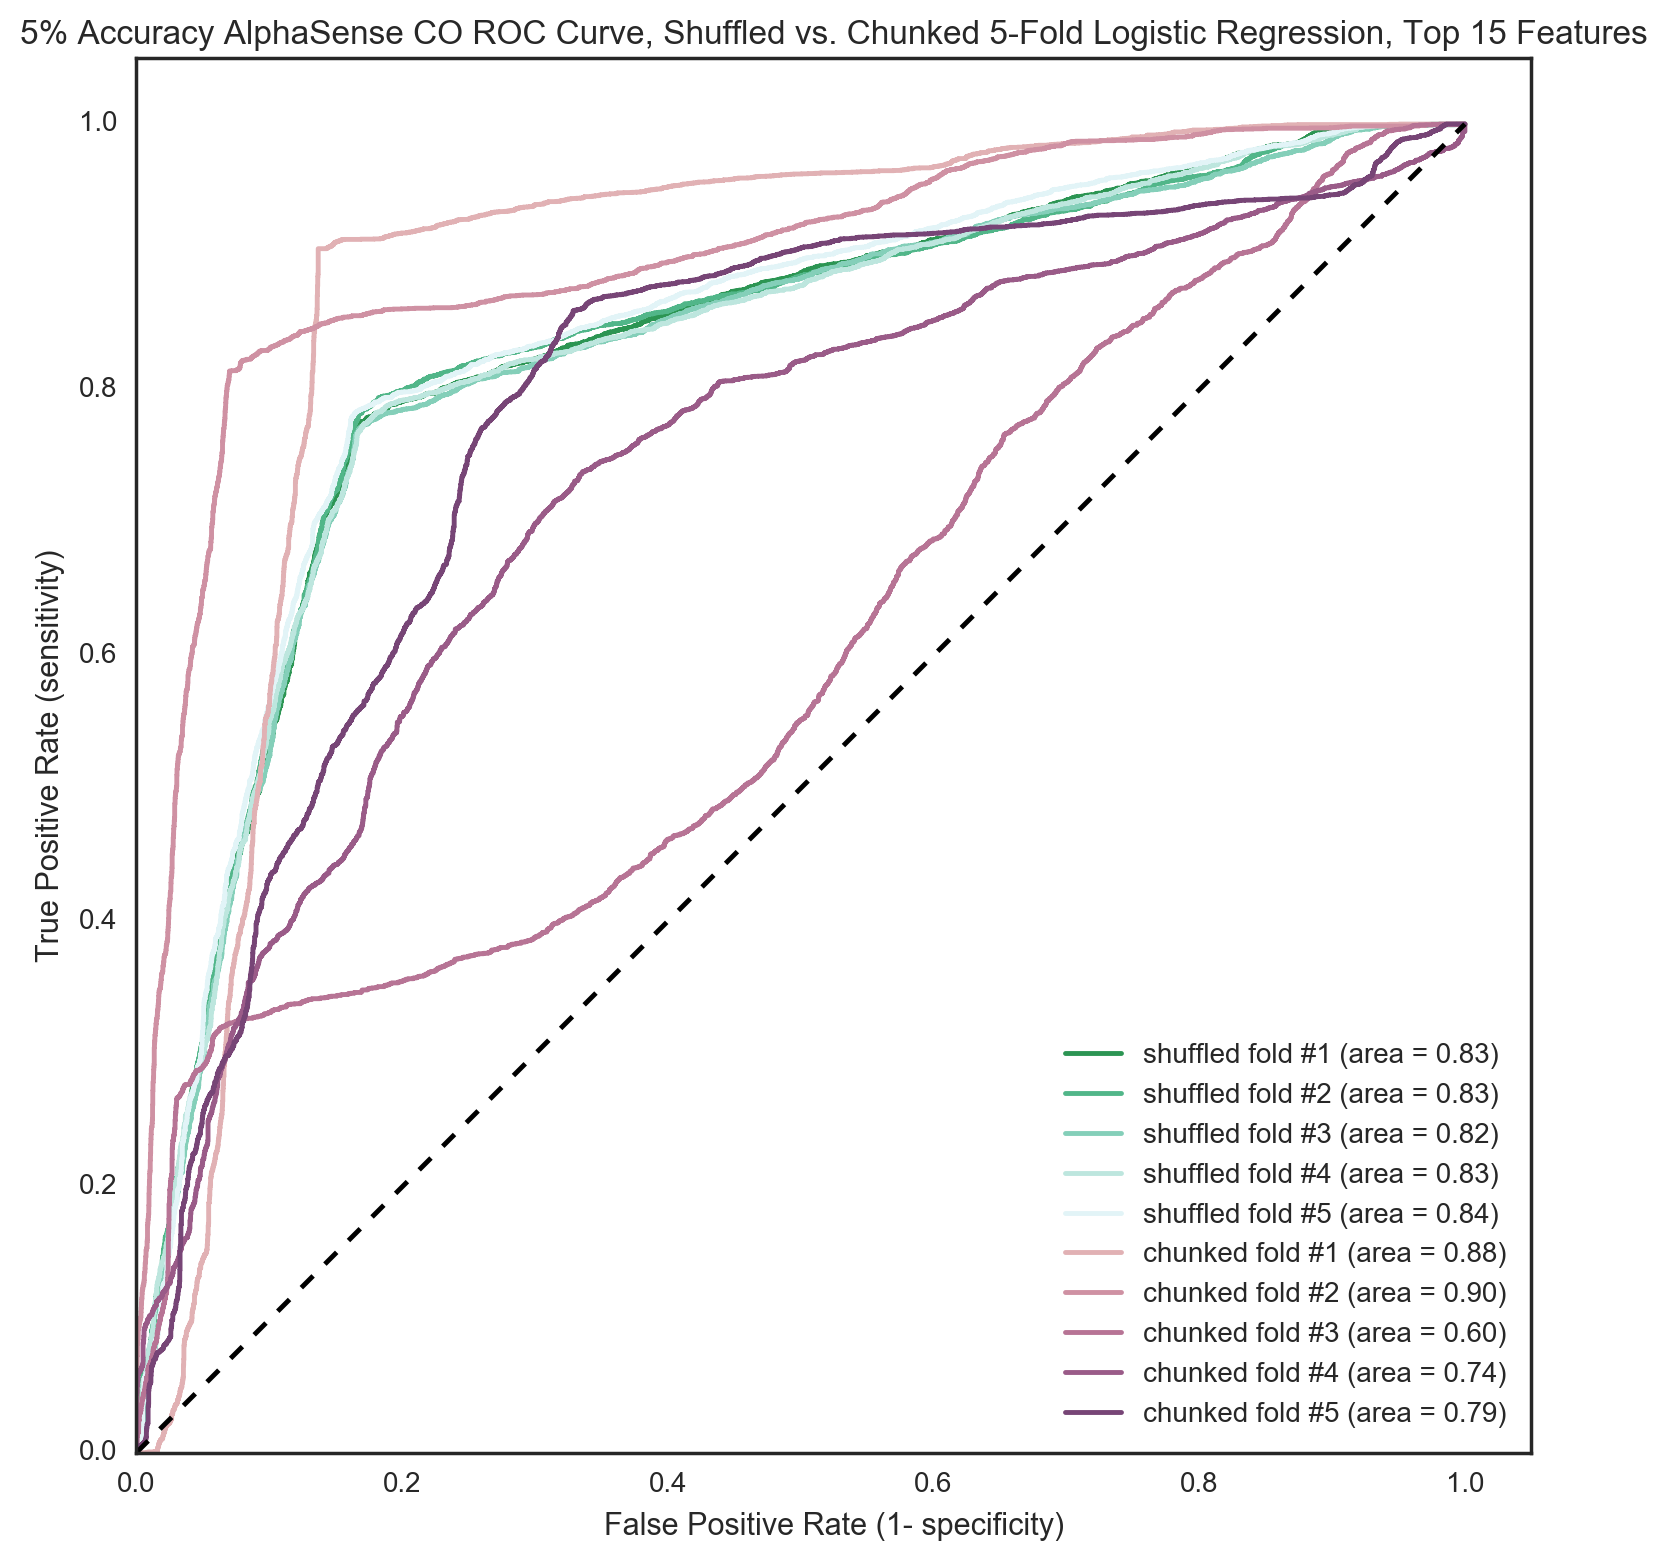
\includegraphics[width=\textwidth]{figs/as1_co_5_roc_pruned_features}               
 	 \caption{AlphaSense CO Sensor #1 ROC Using Top 15 Features}
  	\label{fig:as1_co_5_roc_pruned_features}
\end{figure}



here's text referencing the (Table \ref{tab:as2_o3_randomforest_features}).

\begin{table}[H]
\centering
\small
\begin{tabular}{lllllllll}
\\
\\
\toprule
Feature & Importance \\
\midrule
lmse\_calib\_as\_co & 0.0518584805682 \\
avg\_15\_lmse\_calib\_as\_co & 0.0404238890793 \\
avg\_720\_bkcarbon & 0.0222537733125 \\
avg\_60\_bkcarbon & 0.0216045744972 \\
avg\_1440\_bkcarbon & 0.0198813295966 \\
as\_o3 & 0.0198510401658 \\
lmse\_as\_no2 & 0.0197364055605 \\
avg\_10\_as\_o3 & 0.0196965727088 \\
bkcarbon & 0.0194862747741 \\
as\_no2 & 0.0192353467551 \\
avg\_15\_lmse\_as\_no2 & 0.0180978893662 \\
lmse\_avg\_15\_as\_no2 & 0.0172526534474 \\
avg\_15\_as\_no2 & 0.0162905415767 \\
avg\_15\_as\_co & 0.0158810645781 \\
as\_co & 0.0158442759727 \\
\bottomrule
\end{tabular}
\label{tab:as2_co_randomforest_features}
\caption{Top 15 Features from Random Forest for CO Sensor #2, used in Pruned Logistic Regression}
\end{table}


\begin{figure}[htb]
 	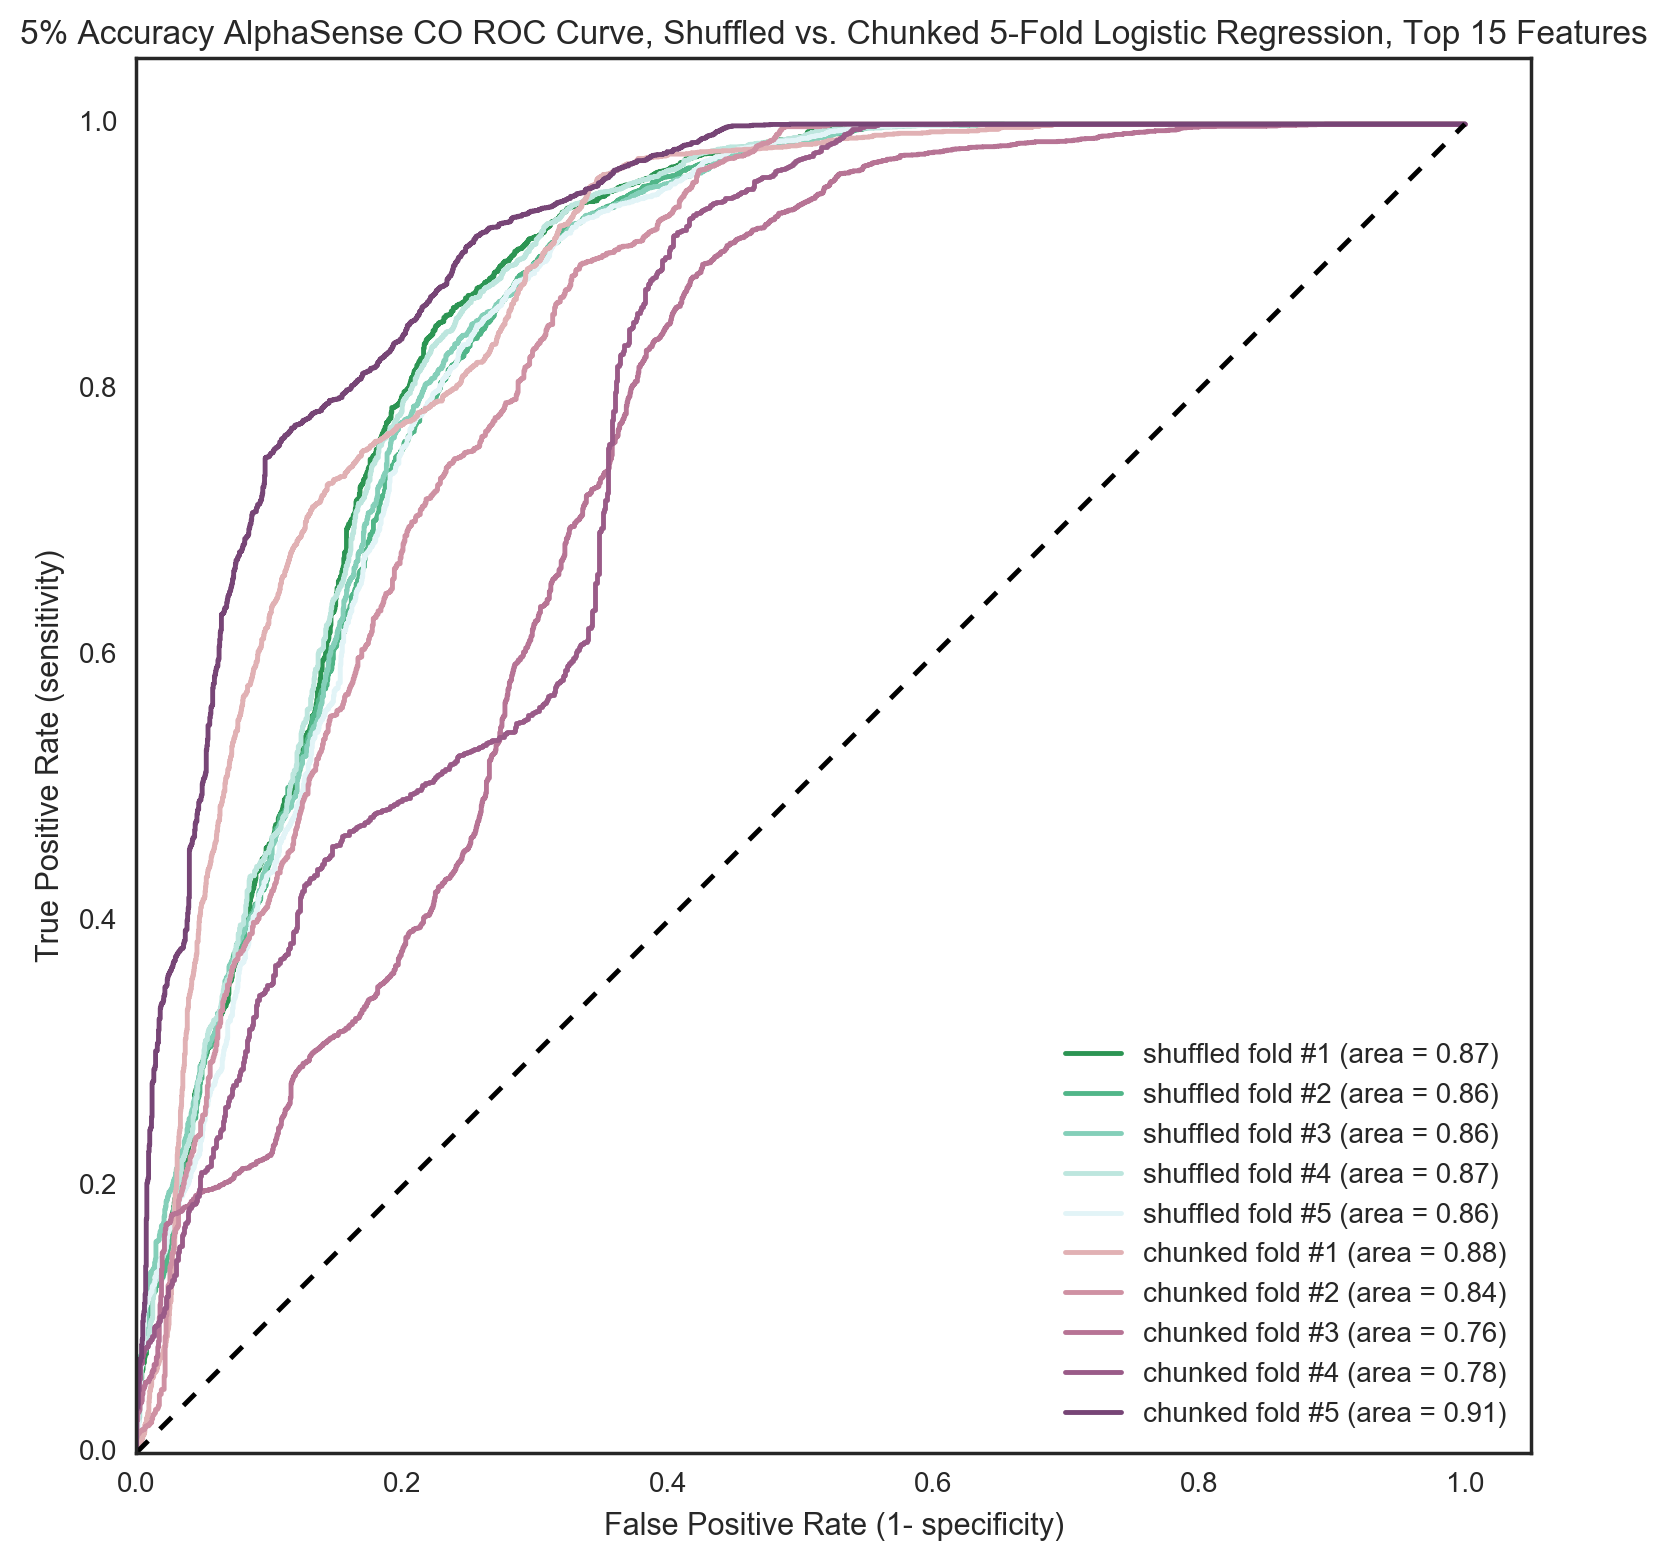
\includegraphics[width=\textwidth]{figs/as2_co_5_roc_pruned_features}               
 	 \caption{AlphaSense CO Sensor #2 ROC Using Top 15 Features}
  	\label{fig:as2_o3_7p5_roc_pruned_features}
\end{figure}

\begin{figure}[htb]
 	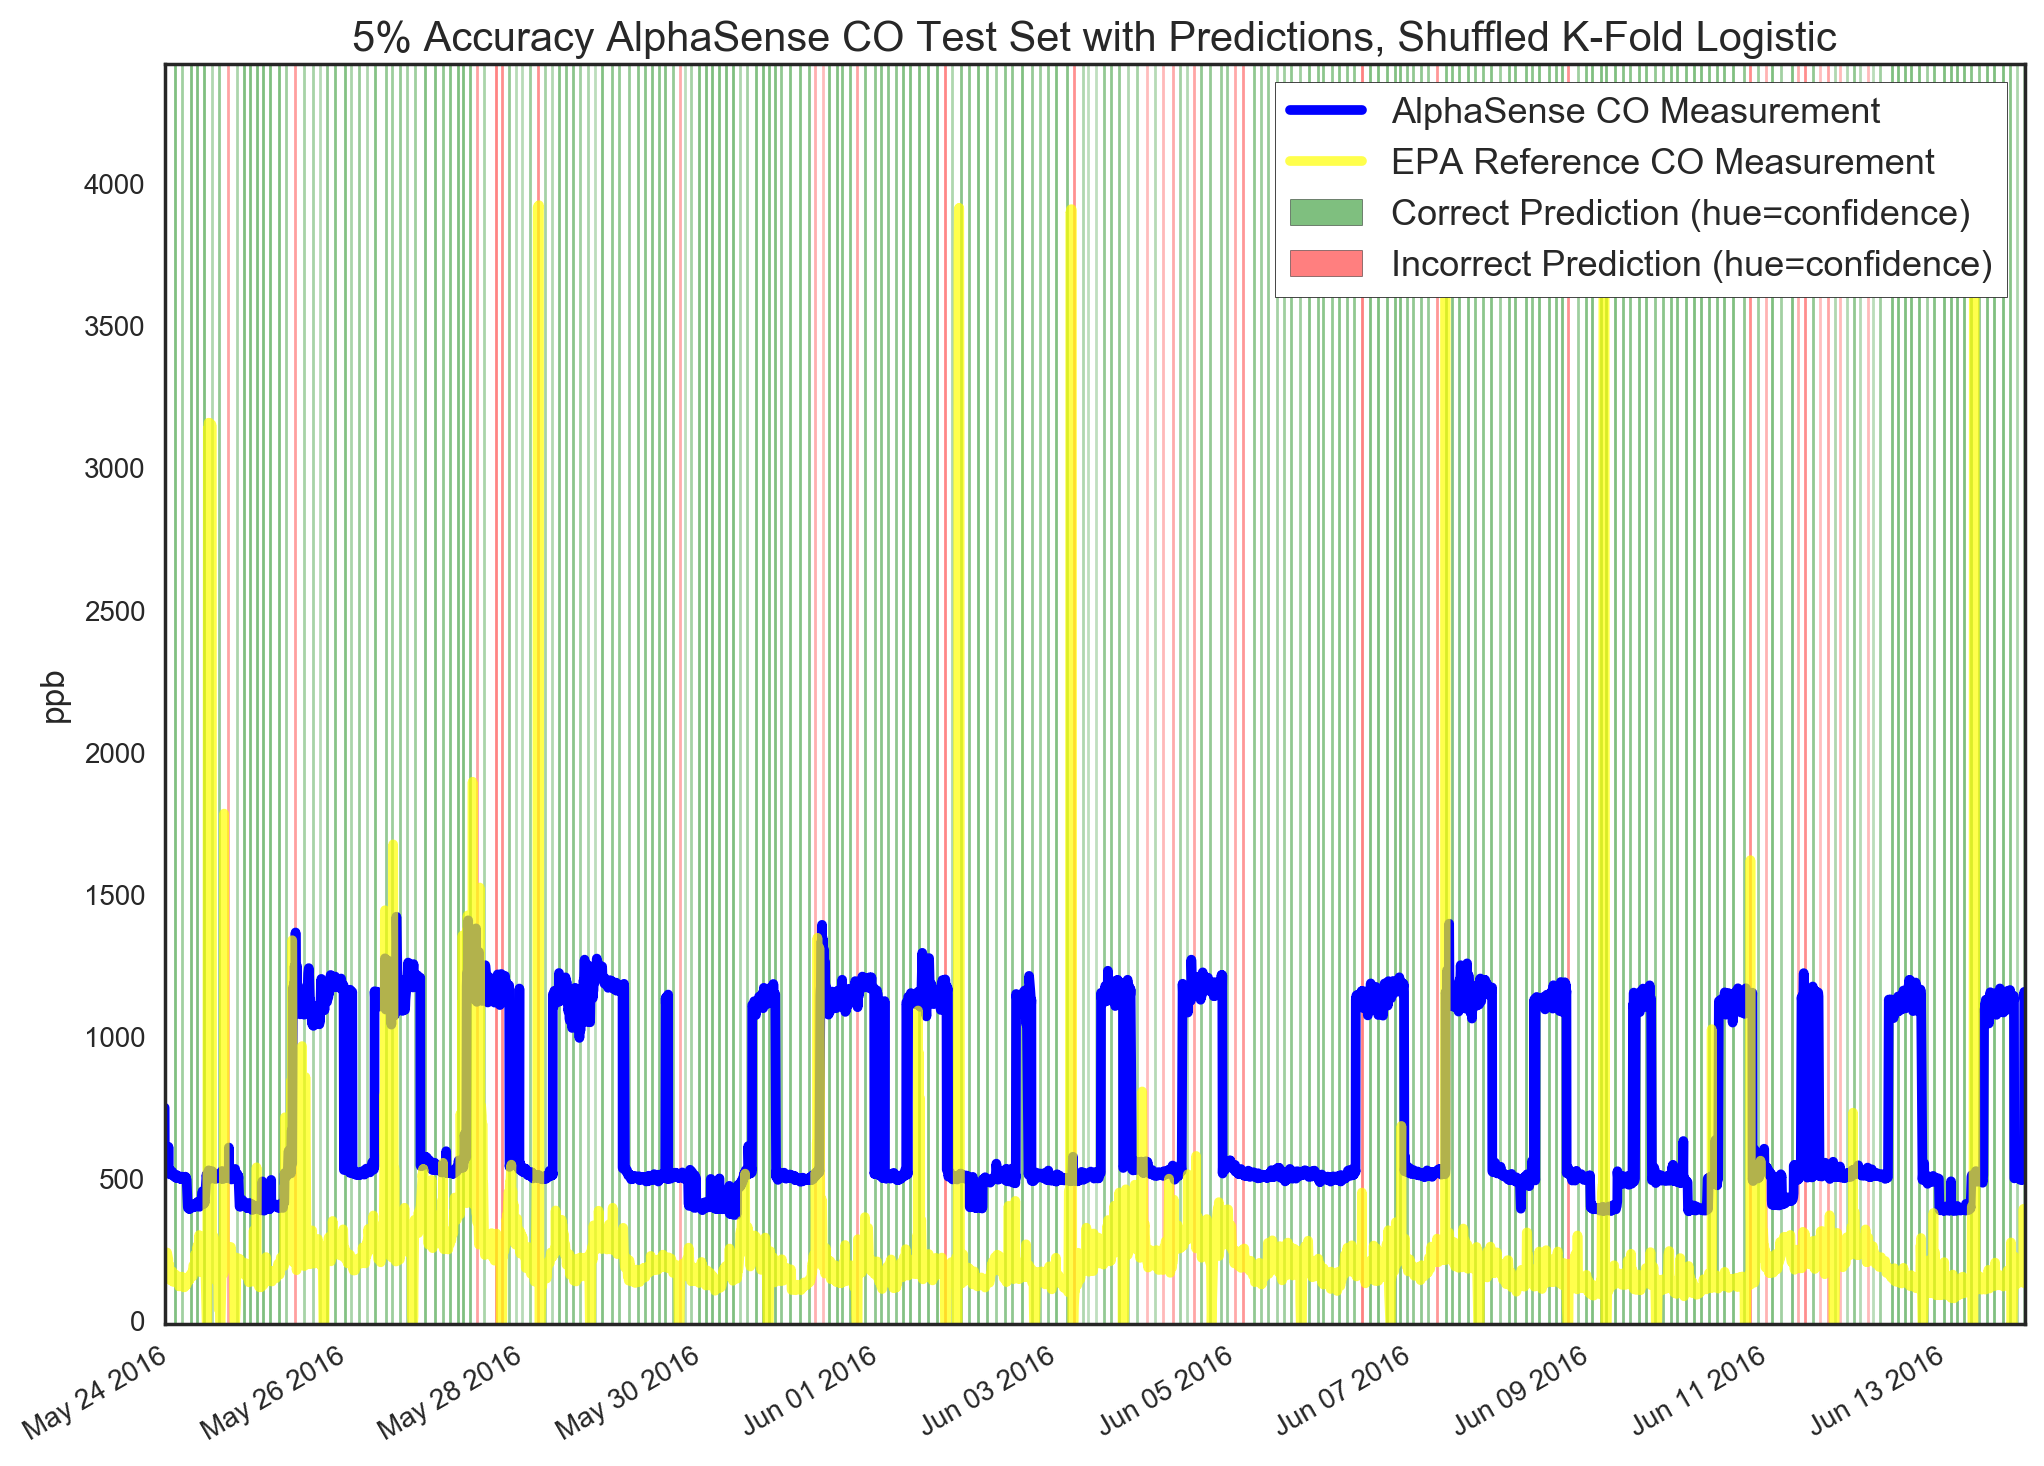
\includegraphics[width=\textwidth]{figs/as2_co_5_logistic_predictions}               
 	 \caption{AlphaSense CO Sensor #2 Prediction Accuracy}
  	\label{fig:as2_co_5_logistic_predictions}
\end{figure}



\FloatBarrier
\section{AlphaSense NO2}
\FloatBarrier

\FloatBarrier
\section{AlphaSense O3}
\FloatBarrier

\clearpage
\newpage
